%% LyX 1.5.1 created this file.  For more info, see http://www.lyx.org/.
%% Do not edit unless you really know what you are doing.
\documentclass[oneside,english,onecolumn]{book}
\usepackage[T1]{fontenc}
\usepackage[utf8]{inputenc}
\usepackage{geometry}
% \geometry{a4paper,tmargin=1in,bmargin=1in,lmargin=1in,rmargin=1in}
\geometry{letterpaper,tmargin=1in,bmargin=1in,lmargin=1in,rmargin=1in}
\setcounter{secnumdepth}{3}
\setcounter{tocdepth}{3}
\usepackage{float}
\usepackage{textcomp}
\usepackage{amsmath}
\usepackage{color}
\usepackage{xcolor}
\usepackage{placeins}

% figures
\usepackage[pdftex]{graphicx}
\usepackage{eso-pic}
\usepackage[position=top,singlelinecheck=false]{subfig}

% we are running pdflatex, so convert .eps files to .pdf
\usepackage{epstopdf}
\usepackage{tikz}
\usepackage{amssymb}
\IfFileExists{url.sty}{\usepackage{url}}
                      {\newcommand{\url}{\texttt}}
\usepackage[authoryear]{natbib}

\usepackage{bibentry}
\nobibliography*

% \renewcommand{\familydefault}{\sfdefault}

\makeatletter

%%%%%%%%%%%%%%%%%%%%%%%%%%%%%% LyX specific LaTeX commands.
\newcommand{\noun}[1]{\textsc{#1}}
%% A simple dot to overcome graphicx limitations
\newcommand{\lyxdot}{.}

%%%%%%%%%%%%%%%%%%%%%%%%%%%%%% Textclass specific LaTeX commands.
\newenvironment{lyxcode}
{\begin{list}{}{
\setlength{\rightmargin}{\leftmargin}
\setlength{\listparindent}{0pt}% needed for AMS classes
\raggedright
\setlength{\itemsep}{0pt}
\setlength{\parsep}{0pt}
\normalfont\ttfamily}%
 \item[]}
{\end{list}}

% figures
\usepackage[dvips]{epsfig}
\usepackage{wrapfig}

% fonts
\usepackage{times}

% hyperlinks to sections and references
\usepackage[colorlinks=true,
            linkcolor=blue,
            urlcolor=blue,
            citecolor=blue,
            pdftex,bookmarks=true,
            bookmarksnumbered=true,
            pdfpagemode=None,
            pdfstartview=FitH,
            pdfpagelayout=SinglePage,
            pdfborder={0 0 0}]{hyperref}

\newcommand{\urlwithparentheses}[1]{(\url{#1})}

% biblio GJI
\bibliographystyle{abbrvnat}

\newcommand{\nexxi}{\mbox{\texttt{NEX\_XI\/}}}
\newcommand{\nexeta}{\mbox{\texttt{NEX\_ETA\/}}}
\newcommand{\nprocxi}{\mbox{\texttt{NPROC\_XI\/}}}
\newcommand{\nproceta}{\mbox{\texttt{NPROC\_ETA\/}}}
\newcommand{\nchunks}{\mbox{\texttt{NCHUNKS\/}}}

\newcommand{\FIG}[1]{figure~\ref{#1}}

\newcommand{\MB}[1]{{\mbox{\mathversion{bold}$#1$}}}

\newcommand{\EQ}[2]{
    \begin{equation}
	\label{#1}
        #2
    \end{equation}
}

\newcommand{\ER}[1]{(\ref{#1})}

\usepackage{babel}
\makeatother

\begin{document}

\thispagestyle{empty}

\sffamily

\AddToShipoutPictureBG*{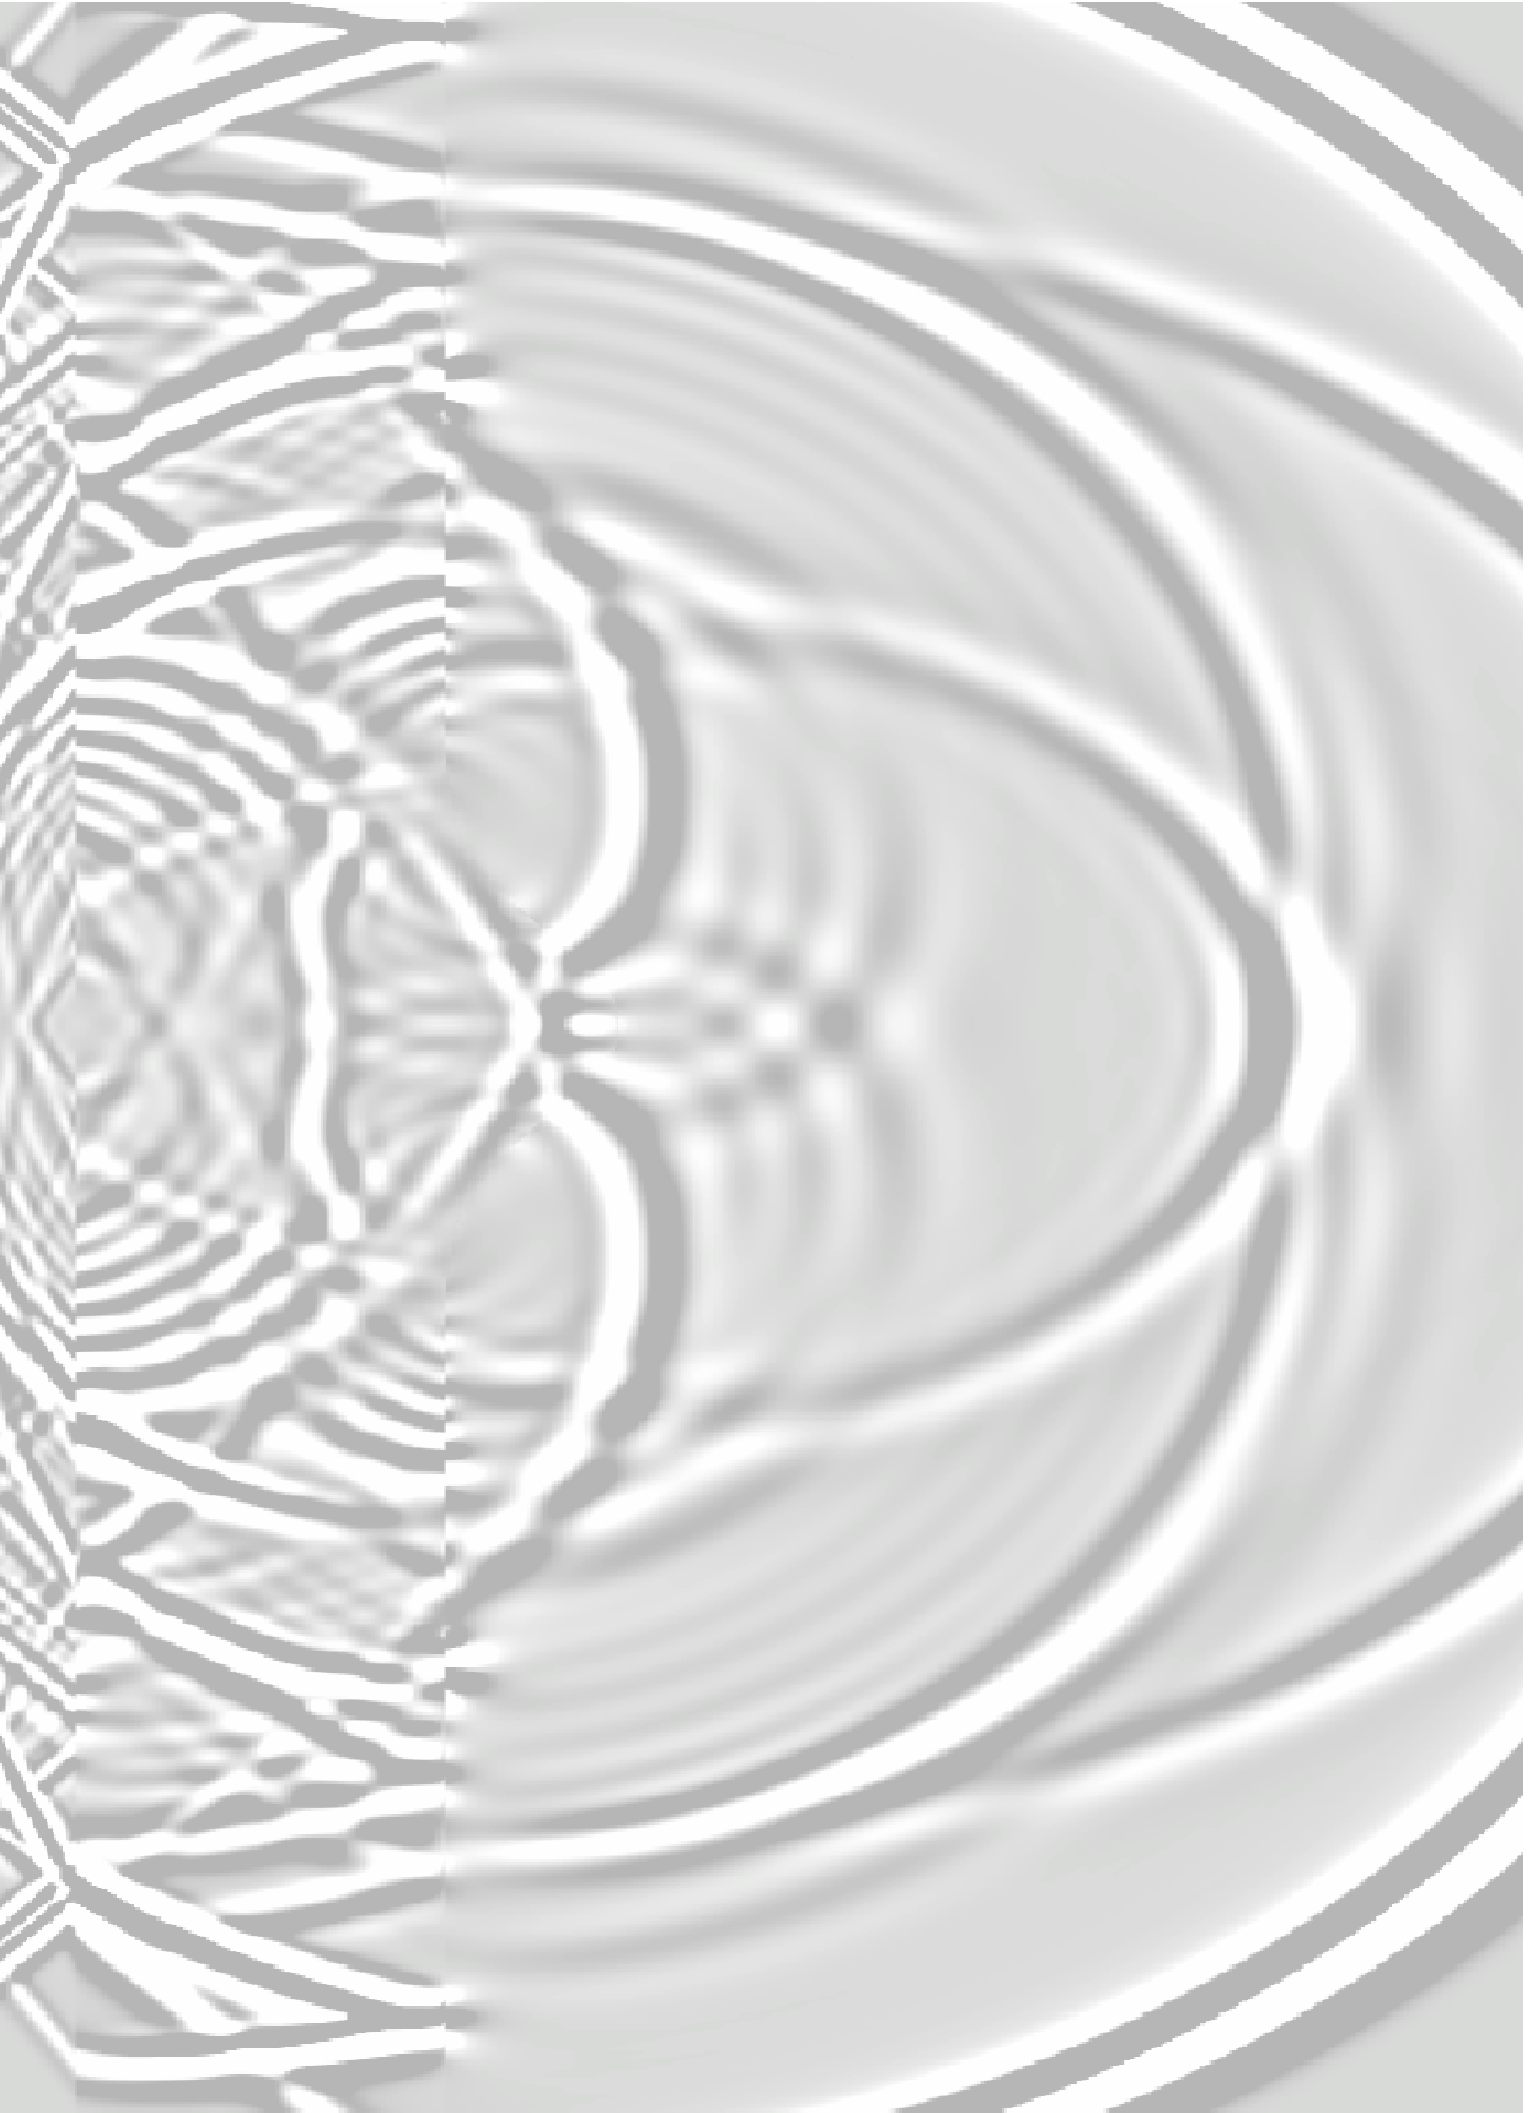
\includegraphics[width=\paperwidth,height=\paperheight]{figures/title_page1.pdf}}

\noindent
\includegraphics[width=1.0\textwidth]{IFOS2D_title1.png}

\vspace{0.3 \textwidth}

\begin{center}
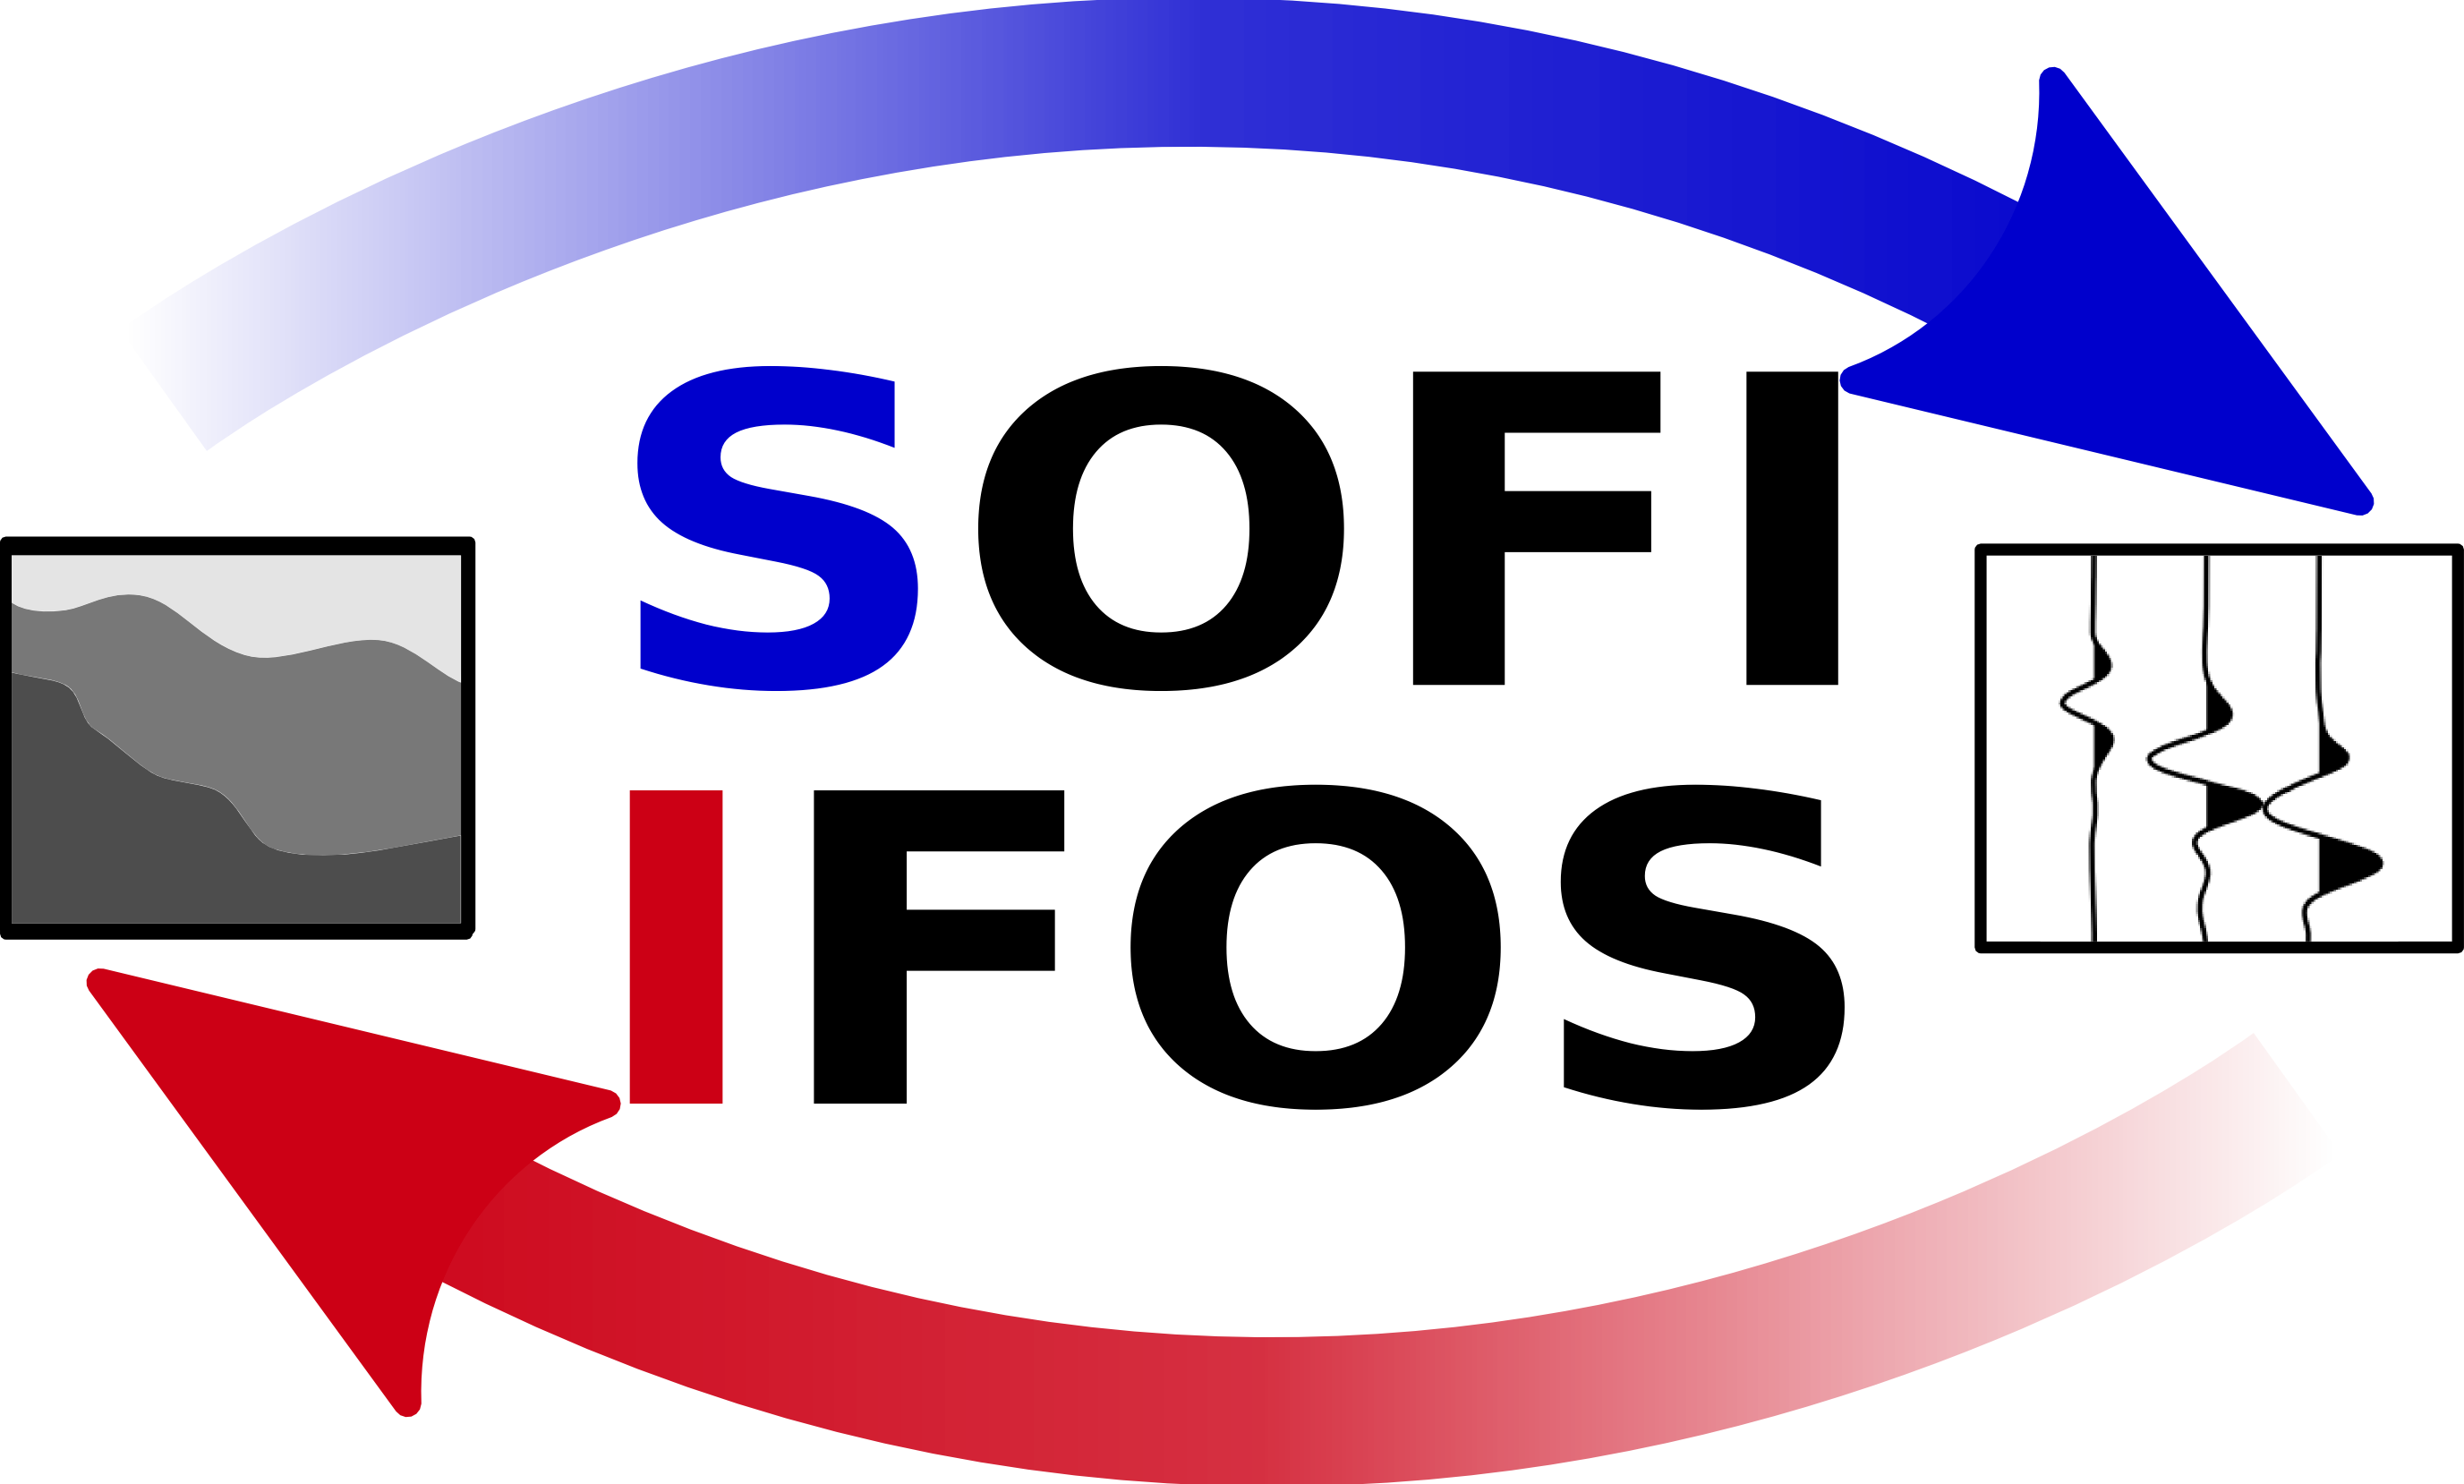
\includegraphics[width=.7\textwidth]{figures/logo_SOFI_IFOS.png}

\vspace{0.2\textwidth}

\end{center}
\rmfamily

\FloatBarrier
\newpage 
\thispagestyle{empty}
\quad 
\newpage
% \maketitle

\section*{Authors}

The IFOS2D code (formerly DENISE) was at first developed by Daniel K\"ohn, Denise De Nil and Andr$\rm{\acute{e}}$ Kurzmann at the Christian-Albrechts-Universit\"at Kiel and TU Bergakademie Freiberg (Germany) from 2005 to 2009.\\
\newline
This documentation was originally written by Daniel K\"ohn.\\ Large parts of the shown theory is extracted from his dissertation \cite{koehn:11}.\\
\newline
The forward code is based on the viscoelastic FD code fdveps (now SOFI2D) by \cite{bohlen:02}.\\
\newline
Different external libraries for time domain filtering are used.\\ 
The copyright of the source codes are held by different persons:\\
\newline
cseife.c, cseife.h, lib\_stfinv, lib\_aff, lib\_fourier:\\ 
Copyright $\copyright$ 2005 by Thomas Forbriger (BFO Schiltach) \\
\newline
cseife\_deriv.c, cseife\_gauss.c, cseife\_rekfl.c, cseife\_rfk.c and cseife\_tides.c:\\
Copyright $\copyright$ 1984 by Erhard Wielandt\\
This algorithm was part of seife.f. A current version of seife.f can be obtained from http://www.software-for-seismometry.de/\\
\newline 
The Matlab implementation of a few SU routines, mainly used to read and write SU files are:\\
Copyright $\copyright$ 2008, Signal Analysis and Imaging Group\\
For more information: http://www-geo.phys.ualberta.ca/saig/SeismicLab\\
Author: M.D.Sacchi\\
\newline

\noindent
Since then it has been developed and maintained by a development team: in alphabetical order,\\
\newline
(up to 2014)\\
Lisa Groos,\\
Sven Heider,\\
Martin Sch\"afer,\\
\newline
(since 2014) \\
Laura Ga\ss ner,\\
Tilman Metz,\\
Niklas Thiel,\\
Florian Wittkamp.\\
% (add other developers here in the future).

\newpage

\section*{License}\label{license}

IFOS2D is free software: you can redistribute it and/or modify it under the terms of the GNU General Public License as published by the Free Software Foundation, version 2.0 of the License only.\\
 \newline
IFOS2D is distributed in the hope that it will be useful, but WITHOUT ANY WARRANTY; without even the implied warranty of MERCHANTABILITY or FITNESS FOR A PARTICULAR PURPOSE. See the GNU General Public License for more details. You should have received a copy of the GNU General Public License along with IFOS2D. See file COPYING and/or \path{http://www.gnu.org/licenses/gpl-2.0.html}.\\
\newline
The Authors of IFOS2D are listed in file \path{AUTHORS}.
%------------------------------------------------------------------------------------------------%
\section*{Acknowledgments}
%------------------------------------------------------------------------------------------------%

We thank for constructive discussions and further code improvements:\\
\newline
Daniel K\"ohn (Christian-Albrechts-Universit\"at Kiel), \\
Anna Przebindowska (Karlsruhe Institute of Technology), \\
Olaf Hellwig (TU Bergakademie Freiberg), \\
Dennis Wilken and Wolfgang Rabbel (Christian-Albrechts-Universit\"at Kiel).
\newline

\noindent The development of the code was supported by the Christian-Albrechts-Universität Kiel, TU Bergakademie Freiberg, Deutsche Forschungsgemeinschaft (DFG), Bundesministerium für Bildung und Forschung (BMBF), the Wave Inversion Technology (WIT) Consortium and the Verbundnetz-Gas AG (VNG).

\noindent The code was tested and optimized at the computing centres of Kiel University, TU Bergakademie Freiberg, TU Chemnitz, TU Dresden, the Karlsruhe Institute of Technology (KIT) and the Hochleistungsrechenzentrum Nord (HLRN 1+2). 
\newline

%------------------------------------------------------------------------------------------------%
\section*{References}
%------------------------------------------------------------------------------------------------%

\,

\noindent\bibentry{koehn:11}\\

\noindent\bibentry{kohn2012influence}\\

\noindent\bibentry{groos2013}\\

\noindent\bibentry{groos2014}\\

\noindent\bibentry{forbriger2014}\\

\noindent\bibentry{schaefer2014a}\\

\noindent\bibentry{schaefer2014}\\

\newpage{}

\tableofcontents{}

\chapter{License}\label{license}

IFOS2D is free software: you can redistribute it and/or modify it under the terms of the GNU General Public License as published by the Free Software Foundation, version 2.0 of the License only.
 
IFOS2D is distributed in the hope that it will be useful, but WITHOUT ANY WARRANTY; without even the implied warranty of MERCHANTABILITY or FITNESS FOR A PARTICULAR PURPOSE. See the GNU General Public License for more details. You should have received a copy of the GNU General Public License along with IFOS2D. See file COPYING and/or \path{http://www.gnu.org/licenses/gpl-2.0.html}.

The Authors of IFOS2D are listed in file \path{AUTHORS}.


%------------------------------------------------------------------------------------------------%

\chapter{Introduction}

%------------------------------------------------------------------------------------------------%

The aim of Full Waveform Tomography (FWT) is to estimate the elastic material parameters in the underground. This can be achieved by minimizing the misfit energy 
between the modeled and field data using a gradient optimization approach. Because the FWT uses the full information content of each seismogram, structures below the seismic 
wavelength can be resolved. This is a tremendous improvement in resolution compared to travel time tomography (\cite{prattgao:2002}).\\ 
The concept of full waveform tomography was originally developed by Albert Tarantola in the  1980s  for the acoustic, isotropic elastic, and 
viscoelastic case (\cite{tarantola:84a,tarantola:84,tarantola:86,tarantola:88}). First numerical implementations were realized at the end of the 1980s 
(\cite{gauthier:86}, \cite{mora:87}, \cite{pica:90}), but due to limited computational resources, the application was restricted to simple 
2D synthetic test problems and small near offset datasets. At the begining of the 1990s the original time domain formulation was transfered 
to a robust frequency domain approach (\cite{prattworth:90}, \cite{pratt:90}). With the increasing performance of supercomputers moderately 
sized problems could be inverted with frequency domain approaches.\\ A spectacular result to prove the application of acoustic FWT on laboratory scale was presented by \cite{pratt:99} for ultrasonic tomography measurements on a simple block model. In a numerical blind test \cite{brenders:2007} achieved a very good agreement between their inversion result and the unkown true P-wave velocity model. The parallelization and performance optimizations of the frequency domain approach (see e.g. \cite{sourbier:09}, \cite{sourbier:09b}) lead to a wide range of acoustic FWT applications for problems on different scales, from the global scale, crustal scale over engineering and near surface scale, down to laboratory scale (\cite{pratt:2004}).\\ Beside the application to geophysical problems, the acoustic FWT is also used to improve the resolution in medical cancer diagnostics (\cite{pratt:2007}). However, all these examples are restricted to the inversion of the acoustic material parameters: P-wave velocity, density and additionally the viscoacoustic damping $\rm{Q_p}$ for the P-waves. Even today the independent 2D FWT of all three isotropic elastic material parameters is still a challenge. Most elastic approaches invert for P-wave velocity only and use empirical relationships to deduce the distribution of S-wave velocity and density (\cite{shipp:02,sheen:06}). Recently some authors also investigated the independent multiparameter FWT in the frequency domain (\cite{choi:2008,choi:2008a,brossier:2009}).  

In order to extract information about the structure and composition of the crust from seismic observations, it is necessary to be able to predict how seismic wavefields are affected by complex structures.
Since exact analytical solutions to the wave equations do not exist for most subsurface configurations, the solutions can be obtained only by numerical methods. For iterative calculations of synthetic seismograms with limited computer resources fast and accurate modeling methods are needed. 

The FD modeling/inversion program IFOS2D (\textbf{I}nversion of \textbf{F}ull \textbf{O}bserved \textbf{S}eismograms), is based on the FD approach described by \cite{virieux:86} and \cite{levander:88}. The present program IFOS2D has the following extensions

\begin{itemize}
\item is efficently parallelized using domain decomposition with MPI (\cite{bohlen:02}),
\item considers viscoelastic wave propagation effects like attenuation and dispersion
(\cite{robertsson:94,blanch:95,bohlen:02}),
\item employs higher order FD operators,
\item applies Convolutional Perfectly Matched Layer boundary conditions at the edges of the numerical mesh (\cite{komatitsch:07}).
\end{itemize}

In the following sections, we give an extensive description of the theoretical background, the different input parameters and show a few benchmark modeling and inversion applications.



%------------------------------------------------------------------------------------------------%

\chapter{Theoretical Background}

%------------------------------------------------------------------------------------------------%

\section{Equations of motion for an elastic medium}\label{elastic_fd_model} 
The propagation of waves in a general elastic medium can be described by a system of coupled linear partial differential equations. They consist of the equations of motion
\EQ{m:1}{\begin{split}
\rm{\rho \frac{\partial v_i}{\partial t}} &\rm{= \frac{\partial \sigma_{ij}}{\partial x_j} + f_i}\\
\end{split}}   
which simply state that the momentum of the medium, the product of density $\rm{\rho}$ and the displacement velocity $\rm{v_i}$, can be changed by surface forces, described by the stress tensor $\rm{\sigma_{ij}}$ or body forces $\rm{f_i}$. These equations describe a general medium, like gas, fluid, solid or plasma. The material specific properties are introduced by additional equations which describe how the medium reacts when a certain force is applied. In the isotropic elastic case this can be described by a linear stress-strain relationship:  
\EQ{m:2}{\begin{split}
\rm{\sigma_{ij}}&\rm{=\lambda \theta \delta_{ij} + 2 \mu \epsilon_{ij}}\\
\rm{\epsilon_{ij}}&\rm{=\frac{1}{2}\biggl(\frac{\partial u_i}{\partial x_j}+\frac{\partial u_j}{\partial x_i}\biggr)}
\end{split}}   
where $\rm{\lambda}$ and $\rm{\mu}$ are the Lam$\rm{\acute{e}}$ parameters, $\rm{\epsilon_{ij}}$ the strain tensor and $\rm{u_i}$ the displacement. Using $\rm{v_i = \frac{\partial u_i}{\partial t}}$, \ER{m:1} and \ER{m:2} can be transformed into a system of second order partial differential equations:
\EQ{2:20}{\begin{split}
\rm{\rho \frac{\partial^2 u_i}{\partial t^2}} &\rm{= \frac{\partial \sigma_{ij}}{\partial x_j} + f_i}\\
\rm{\sigma_{ij}}&\rm{=\lambda \theta \delta_{ij} + 2 \mu \epsilon_{ij}}\\
\rm{\epsilon_{ij}}&\rm{=\frac{1}{2}\biggl(\frac{\partial u_i}{\partial x_j}+\frac{\partial u_j}{\partial x_i}\biggr)}
\end{split}}
This expression is called {\bf{Stress-Displacement}} formulation. Another common form of the elastic equations of motion can be deduced by taking the time derivative of the stress-strain relationship and the strain tensor in Eq. \ER{2:20}. Since the Lam$\acute{\rm e}$ parameters $\rm{\lambda}$ and $\rm{\mu}$ do not depend on time, Eq. \ER{2:20} can be written as:
\EQ{2:20:1}{\begin{split}
\rm{\rho \frac{\partial v_i}{\partial t}} &\rm{= \frac{\partial \sigma_{ij}}{\partial x_j} + f_i}\\
\rm{\frac{\partial \sigma_{ij}}{\partial t}} &\rm{= \lambda \frac{\partial \theta}{\partial t} \delta_{ij} + 2 \mu \frac{\partial \epsilon_{ij}}{\partial t}}\\
\rm{\frac{\partial \epsilon_{ij}}{\partial t}}&\rm{=\frac{1}{2}\biggl(\frac{\partial v_i}{\partial x_j}+\frac{\partial v_j}{\partial x_i}\biggr)}
\end{split}}  
This expression is called {\bf{Stress-Velocity}} formulation. For simple cases \ER{2:20} and \ER{2:20:1} can be solved analytically. More complex problems require numerical solutions. One possible approach for a numerical solution is described in the next section.
\newpage
\section{Solution of the elastic wave equation by finite differences}\label{elastic_FD_Code}
\subsection{Discretization of the wave equation}
For the numerical solution of the elastic equations of motion, Eqs. \ER{2:20} have to be discretized in time and space on a grid. The
particle velocity $\rm{\mathbf{v}}$, the stresses $\rm{\sigma_{ij}}$, the Lam$\acute{\rm e}$ parameters $\rm{\lambda}$ and $\rm{\mu}$ are calculated and defined at discrete Cartesian coordinates $\rm{x=i\; dh}$, $\rm{y=j\; dh}$ and discrete times $\rm{t=n\; dt}$. 
$\rm{dh}$ denotes the spatial distance between two adjacent grid points and $\rm{dt}$ the difference between two successive time steps. Therefore every grid point is located in the interval  $\rm{i \in N | [1,NX]}$, $\rm{j \in N | [1,NY]}$ and $\rm{n \in N | [1,NT]}$, where
$\rm{NX}$, $\rm{NY}$ and $\rm{NT}$ are the number of discrete spatial grid points and time steps, respectively. Finally the partial derivatives are replaced by {\bf{finite-difference} (FD)} operators. 
Two types of operators can be distinguished, forward and backward operators $\rm{D^+,\;D^-}$. The derivative of a function y with respect to a variable x can be approximated by the following operators:  
\EQ{disc:1}{\begin{split}
\rm{D^+_x y}&\rm{= \frac{y[i+1]-y[i]}{dh} \hspace{1 cm} \text{forward operator}}\\
\rm{D^-_x y}&\rm{= \frac{y[i]-y[i-1]}{dh} \hspace{1 cm} \text{backward operator}}\\
\end{split}}\\
To calculate the spatial derivatives of the wavefield variables at the correct positions, the variables are not placed on the same 
grid points, but staggered by half of the spatial grid point distance (\cite{virieux:86} and \cite{levander:88}). 
\FIG{SSG-Cart.eps} shows the distribution of the material parameters and wavefield variables on the spatial grid. 


\begin{figure}[bh]
\begin{center}
\begin{tikzpicture}[scale=6]

\draw[thick,->] (0,0,0) -- (1.2,0,0) node[anchor=north]{$\rm x$};
\draw[thick,->] (0,0,0) -- (0,-1.2,0) node[anchor=west]{$\rm y$};

\draw (0.5,0,0) -- (0.5,-0.5,0);
\draw (0,-0.5,0) -- (0.5,-0.5,0);

\draw[line width=2pt,color=black] (0.49,-0.51) -- (0.51,-0.51) -- (0.51,-0.49) -- (0.49,-0.49) -- cycle;
\draw[line width=2pt,color=black] (0.49,-0.01) -- (0.51,-0.01) -- (0.50,0.01) -- cycle;
\draw[line width=2pt,color=black] (-0.01,-0.49) -- (0.01,-0.49) -- (0.00,-0.51) -- cycle;

\fill[black] (0,0,0) circle (0.6pt) node [anchor=south]{$\rm (i,j)$} node 
[anchor=north west]{$\rm \sigma_{xx}$, $\sigma_{yy}$};
\fill[black] (0,-0.07,0) node [anchor=north west]{$\rm\rho$, $\lambda$, $\mu$};

\fill (0,-1,0) circle (0.5pt) node [anchor=west]{$\rm (i,j+1)$};
\fill (1,0,0) circle (0.5pt) node [anchor=south]{$\rm (i+1,j)$};

\fill[black] (0.5,0,0)  node [anchor=north 
west]{$\rm v_{x}$, $\rm\rho_x$};
\fill[black] (0,-0.5,0)  node [anchor=north 
west]{$\rm v_{y}$, $\rm\rho_y$};
\fill[black] (0.5,-0.5,0) circle (0.2pt) node [anchor=north 
west]{$\rm\sigma_{xy}$, $\mu_{xy}$};

\fill[black] (0.8,-0.8,0) node [anchor=north 
west]{$\rm\lambda=\rho\left(v_p^2-2v_s^2\right)$};
\fill[black] (0.8,-0.95,0) node [anchor=north west]{$\rm\mu=\rho v_s^2$};

\end{tikzpicture}
\caption{\label{SSG-Cart.eps} Grid geometry for a standard staggered grid (SSG) in Cartesian coordinates as suggested by 
\cite{virieux:86} and \cite{levander:88}.}
\label{fig_cell}
\end{center}
\end{figure}  

% \caption[Staggered Grid]{Cell of the SSG with elastic 
%  modelling parameters. Stress tensor elements 
% $\sigma_{ij}$, seismic velocities $v_i$ and modell 
% parameters $\lambda$, $\mu$ and $\rho$.}
% \end{figure}
 
% \begin{figure}[bh]
% \begin{center}
% 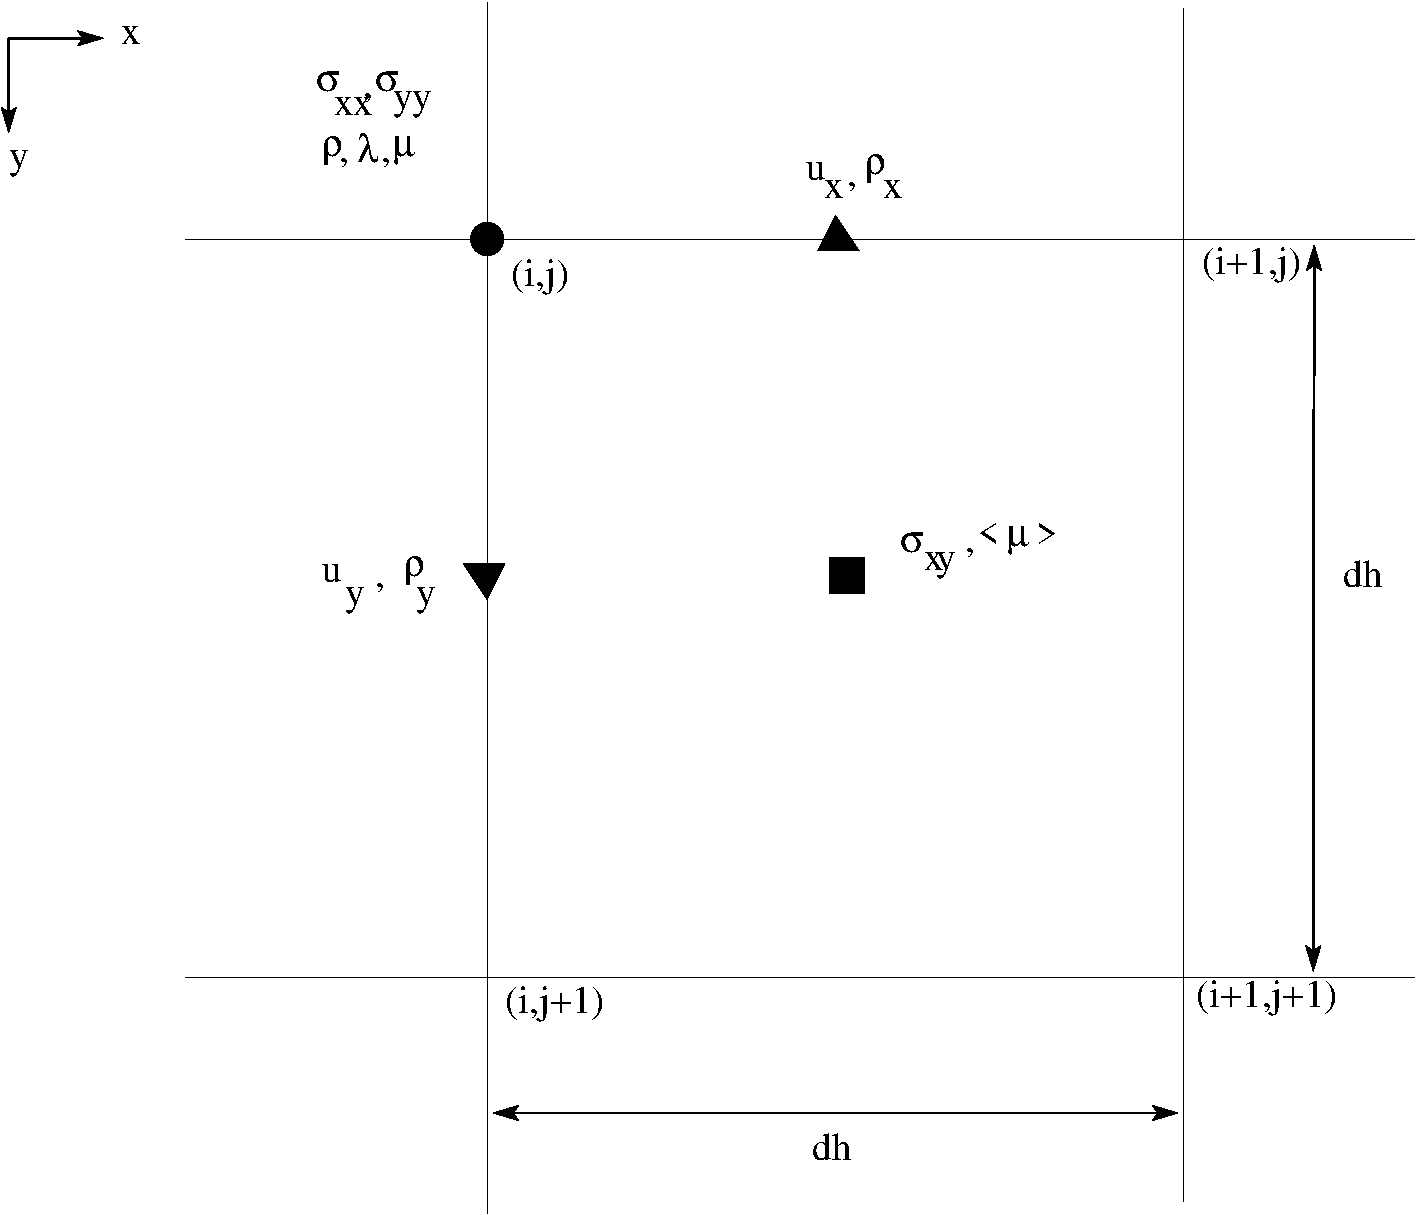
\includegraphics[width=.6\textwidth]{figures/SSG-Cart}
% \caption{\label{SSG-Cart.eps} Grid geometry for a standard staggered grid (SSG) in Cartesian coordinates as suggested by 
% \cite{virieux:86} and \cite{levander:88}.}
% \label{fig_cell}
% \end{center}
% \end{figure}   

To guarantee the stability of the {\bf{standard staggered grid (SSG)}} code, the Lam$\acute{\rm e}$ parameter $\rm{\mu}$ and density $\rm{\rho}$ have to be averaged 
harmonically and arithmetically (\cite{moczo:04}, \cite{bohlen:06}), respectively
\EQ{disc:2}{\begin{split}
\rm{\mu_{xy}[j+\frac{1}{2}][i+\frac{1}{2}]}&\rm{=\biggl[\frac{1}{4}\biggl(\mu^{-1}[j][i]+\mu^{-1}[j][i+1]+\mu^{-1}[j+1][i+1]+\mu^{-1}[j+1][i]\biggr)\biggr]^{-1}}\\ 
\rm{\rho_x[j][i+\frac{1}{2}]}&\rm{=\frac{1}{2}(\rho[j][i+1]+\rho[j][i])}\\
\rm{\rho_y[j+\frac{1}{2}][i]}&\rm{=\frac{1}{2}(\rho[j+1][i]+\rho[j][i])}\\
\end{split}}  
The discretization of the linear stress velocity relationship in \ER{2:20:1} at time step n leads to the following system of equations: % (for simplicity I skip the time index n): 
\EQ{cart_dis:1}{\begin{split}
\rm{v_{xx}[j][i]}&\rm{\approx \frac{v_x[j][i+\frac{1}{2}]-v_x[j][i-\frac{1}{2}]}{dh}}\\ 
\rm{v_{yy}[j][i]}&\rm{\approx \frac{v_y[j+\frac{1}{2}][i]-v_y[j-\frac{1}{2}][i]}{dh}}\\ 
\rm{v_{yx}[j+\frac{1}{2}][i+\frac{1}{2}]}&\rm{\approx \frac{v_y[j+\frac{1}{2}][i+1]-v_y[j+\frac{1}{2}][i]}{dh}}\\ 
\rm{v_{xy}[j+\frac{1}{2}][i+\frac{1}{2}]}&\rm{\approx \frac{v_x[j+1][i+\frac{1}{2}]-v_x[j][i+\frac{1}{2}]}{dh}}\\ 
\rm{\sigma^{n+1}_{xy}[j+\frac{1}{2}][i+\frac{1}{2}]}&\rm{=\sigma^{n}_{xy}[j+\frac{1}{2}][i+\frac{1}{2}] + dt\cdot\mu_{xy}[j+\frac{1}{2}][i+\frac{1}{2}]\biggl(v_{xy}[j+\frac{1}{2}][i+\frac{1}{2}] + v_{yx}[j+\frac{1}{2}][i+\frac{1}{2}]\biggr)}\\ 
\rm{\sigma^{n+1}_{xx}[j][i]}&\rm{= \sigma_{xx}^{n}[j][i] + dt\cdot\lambda[j][i]\cdot \biggl(v_{xx}[j][i] + v_{yy}[j][i] \biggr) + 2 dt\cdot  \mu_{xy}[j][i] \cdot  v_{xx}[j][i]}\\ 
\rm{\sigma^{n+1}_{yy}[j][i]}&\rm{= \sigma_{yy}^{n}[j][i] + dt\cdot\lambda[j][i]\cdot \biggl(v_{xx}[j][i] + v_{yy}[j][i] \biggr) + 2 dt\cdot  \mu_{xy}[j][i] \cdot  v_{yy}[j][i]}\\ 
\end{split}} 
 
The discretization of the momentum equation in \ER{2:20:1} leads to the following system of equations:
\EQ{cart_dis:2}{\begin{split}
\rm{vtt_x^n[j][i+\frac{1}{2}]} &\rm{= \biggl(\sigma_{xx}[j][i+1] - \sigma_{xx}[j][i] + \sigma_{xy}[j+\frac{1}{2}][i] - \sigma_{xy}[j-\frac{1}{2}][i] \biggr)}\\
\rm{vtt_y^n[j+\frac{1}{2}][i]} &\rm{= \biggl(\sigma_{xy}[j][i+\frac{1}{2}] - \sigma_{xy}[j][i-\frac{1}{2}] + \sigma_{yy}[j+1][i] - \sigma_{yy}[j][i] \biggr)}\\ 
\rm{v_x^{n+1}[j][i+\frac{1}{2}]}&\rm{= v_x^{n}[j][i+\frac{1}{2}] + \frac{dt}{dh\cdot \rho_x[j][i+\frac{1}{2}]}\cdot vtt_x^n[j][i+\frac{1}{2}]}\\
\rm{v_y^{n+1}[j+\frac{1}{2}][i]}&\rm{= v_y^{n}[j+\frac{1}{2}][i] + \frac{dt}{dh\cdot \rho_y[j+\frac{1}{2}][i]}\cdot vtt_y^n[j+\frac{1}{2}][i]}\\ 
\end{split}} 
\subsection{Accuracy of FD operators}
The derivation of the FD operators in the last section was a simple replacement of the partial derivatives by finite differences. In the following more systematic approach, the first derivative of a variable f at a grid point i is estimated by a Taylor series expansion (\cite{jastram:92a}):
\EQ{op_acc:1}{\begin{split}
\rm{(2k-1)\frac{\partial f}{\partial x}\biggr|_i}&\rm{=\frac{1}{dh}(f_{i+(k-1/2)}-f_{i-(k-1/2)})}\\
&\rm{+\frac{1}{dh}\sum_{l=2}^N \frac{((k-\frac{1}{2}) dh)^{2l-1}}{(2l-1)!}\frac{\partial^{(2l-1)}f}{\partial
x^{(2l-1)}}\biggr|_i+{\mathcal{O}}(dh)^{2N}} \notag
\end{split}}
For an operator with length 2N, N equations are added with a weight $\rm{\beta_k}$:
\EQ{op_acc:2}{\begin{split}
\rm{[\sum_{k=1}^{N} \beta_k (2k-1)]\frac{\partial f}{\partial x}\biggr|_i}&\rm{=\frac{1}{dh} \sum_{k=1}^{N} \beta_k (f_{i+(k-1/2)}-f_{i-(k-1/2)})}\\
&\rm{+\frac{1}{dh}\sum_{k=1}^{N} \sum_{l=2}^N \beta_k \frac{((k-\frac{1}{2}) dh)^{2l-1}}{(2l-1)!}\frac{\partial^{(2l-1)}f}{\partial
x^{(2l-1)}}\biggr|_i+{\mathcal{O}}(dh)^{2N}}
\end{split}}
The case N=1 leads to the FD operator derived in the last section, which has a length of 2N=2. The Taylor series is truncated after the first term ($\rm{{\mathcal{O}}(dh)^{2}}$). 
Therefore this operator is called {\bf{2nd order FD operator}} which refers to the truncation error of the Taylor series and not to the order of the approximated derivative.
To understand equation \ER{op_acc:2} better, we estimate a {\bf{4th order FD operator}}. This operator has the length 2N = 4 or N=2. The sums in Eq. \ER{op_acc:2} lead to:
\EQ{op_acc:3}{\begin{split}
\rm{(\beta_1+3 \beta_2) \frac{\partial f}{\partial x}\biggr|_i}&\rm{=\frac{1}{dh}(\beta_1(f_{i+1/2}-f_{i-1/2})+\beta_2(f_{i+3/2}-f_{i-3/2}))}\\
&\rm{+\frac{dh^3}{dh}\biggl[\beta_1\frac{1}{8 \cdot 3!}+\beta_2\frac{27}{8 \cdot 3!}\biggr]\frac{\partial^3 f}{\partial x^3}\biggr|_i}
\end{split}}
The weights $\rm{\beta_k}$ can be calculated by the following approach: 
The factor in front of the partial derivative on the LHS of Eq. \ER{op_acc:3} should equal 1, therefore
\EQ{op_acc:4}{\rm{(\beta_1+3\beta_2)=1 \notag.}}
The coefficients in front of $\rm{\frac{\partial^3 f}{\partial x^3}\biggr|_i}$ on the RHS of Eq. \ER{op_acc:3} should vanish:
\EQ{op_acc:5}{\rm{(\beta_1+27\beta_2)=0 \notag.}}
The weights $\rm{\beta_k}$ can be estimated by solving the matrix equation:
\EQ{op_acc:6}{
\rm{\left(
\begin{array}{ll}
1 & 3 \\
1 & 27 \\
\end{array}
\right)\cdot \hspace{0.2 cm}
\left(
\begin{array}{l}
\beta_1 \\
\beta_2 \\
\end{array}
\right)
=
\left(
\begin{array}{l}
1 \\
0 \\
\end{array}
\right) \notag}
}
The resulting coefficients are $\rm{\beta_1=9/8}$ and $\rm{\beta_2=-1/24}$. Therefore the 4th order backward- and forward operators are:
\EQ{op_acc:7}{\begin{split}
\rm{\frac{\partial f}{\partial x}\biggr|_{i+1/2}}&\rm{=\frac{1}{dh}[\beta_1 (f_{i+1}-f_i)+\beta_2 (f_{i+2}-f_{i-1})] \hspace{1 cm} \text{forward operator}}\\
\rm{\frac{\partial f}{\partial x}\biggr|_{i-1/2}}&\rm{=\frac{1}{dh}[\beta_1 (f_{i}-f_{i-1})+\beta_2 (f_{i+1}-f_{i-2})] \hspace{1 cm} \text{backward operator}}\\
\end{split}}
The coefficients $\rm{\beta_i}$ in the FD operator are called {\bf{Taylor coefficients}}. 
%Generally the Taylor coefficients can be calculated using the recursive equation (\cite{liu:2009})
%\EQ{op_acc:8}{\begin{split}
%\rm{\beta_i}&\rm{=\frac{(-1)^{i+1}}{i^2}\prod_{1 \le n \le 2N, n \ne i} \biggl|\frac{n^2-1}{n^2-i^2}\biggr| \; (i=1,2,...,2N).}\\
%\end{split}}
The accuracy of higher order FD operators can be improved by seeking for FD coefficients $\rm{\beta_k}$ that approximate the first derivative in a certain frequency range (\cite{holberg:87}). These numerically optimized coefficients are called {\bf{Holberg coefficients}}.

\subsection{Initial and Boundary Conditions}\label{bound_cond}
To find a unique solution of the problem, initial and boundary conditions have to be defined. The initial conditions for the elastic forward problem are:
\EQ{ini:1}{\begin{split}
\rm{u_i(\mathbf{x},t)} &\rm{= 0}\\
\rm{\frac{\partial u_i(\mathbf{x},t)}{\partial t}} &\rm{= 0}\\
\end{split}}
for all $\rm{x \in V}$ at $\rm{t=0}$. \\
For the geophysical application two types of boundary conditions are very important:
\begin{enumerate}
\item \underline{Horizontal Free Surface:}
The interface between the elastic medium and air at the surface is very important when trying to model surface waves or multiple reflections 
in a marine environment. Since all stresses in the normal direction at this interface vanish
\EQ{free:1}{\rm{\sigma_{xy} = \sigma_{yy}  = 0.0}}
this boundary condition is called (stress) {\bf{free surface}}. 
Two types of implementations are common. In the implicit defintion of the free surface, a small layer with the acoustic parameters of air 
($\rm{V_p=300\;m/s}$, $\rm{V_s=0.0\;m/s}$, $\rm{\rho=1.25\;kg/m^3}$) is placed on top of the model. One advantage of the implicit definition 
of the free surface is the easy implementation of topography on the FD grid, however to get accurate results for surface waves or multiples, 
this approach requires a fine spatial sampling of the FD grid near the free surface. An explicit free surface can be implemented by using 
the mirroring technique by Levander, which leads to stable and accurate solutions for plain interfaces (\cite{levander:88}, \cite{robertsson:95}). If the planar free surface is located at grid point $j=h$, the stress at this point is set to zero and the stresses below the free surface are mirrored with an inverse sign:
\EQ{free:2}{\begin{split}
\rm{\sigma_{yy}(h,i)} &\rm{= 0} \\
\rm{\sigma_{yy}(h-1,i)} &\rm{= - \sigma_{yy}(h+1,i)}\\
\rm{\sigma_{xy}(h-\frac{1}{2},i+\frac{1}{2}) }&\rm{= - \sigma_{xy}(h+\frac{1}{2},i+\frac{1}{2})}\\
\rm{\sigma_{xy}(h-\frac{3}{2},i+\frac{1}{2})} &\rm{= - \sigma_{xy}(h+\frac{3}{2},i+\frac{1}{2})}\\
\end{split}} 
When updating the stress component $\rm{\sigma_{xx}=dt (\lambda + 2 \mu) v_{xx} + dt \lambda v_{yy}}$ at the free surface, only horizontal particle velocities should be used because vertical derivatives over the free surface lead to instabilities (\cite{levander:88}). The vertical derivative of the y-velocity $\rm{v_{yy}}$ can be replaced by using the boundary condition at the free surface: 
\EQ{free:3}{\begin{split}
\rm{\sigma_{yy}} &\rm{= dt (\lambda + 2 \mu) v_{yy} + dt \lambda v_{xx} = 0} \\ 
\rm{v_{yy}} &\rm{= - \frac{\lambda}{(\lambda + 2 \mu)} v_{xx}} \\
\end{split}} 
Therefore the stress $\rm{\sigma_{xx}}$ can be written as
\EQ{free:4}{\begin{split}
\rm{\sigma_{xx}=\frac{4 dt(\lambda \mu + \mu^2)}{\lambda + 2\mu} v_{xx}} 
\end{split}}       
\item \underline{Absorbing Boundary Conditions:}
Due to limited computational resources, the FD grid has to be as small as possible. To model problems with an infinite extension in different directions, e.g. a full or half-space problem,  an artificial absorbing boundary condition has to be applied. A very effective way to damp the waves near the boundaries are {\bf{Perfectly Matched Layers (PMLs)}}. This can be achieved by a coordinate stretch of the wave equations in the
frequency domain (\cite{komatitsch:07}). The coordinate stretch creates exponentially decaying plane wave solutions in the absorbing boundary frame. The PML's are only
reflectionless if the exact wave equation is solved. As soon as the problem is discretized (for example using finite differences) you are solving an approximate wave equation and
the analytical perfection of the PML is no longer valid. To overcome this shortcoming the wavefield is damped by the damping function 
\EQ{FD:6:1}{\rm{c=-V_{pml}\cdot\frac{log(\alpha)}{L}}}
where $\rm{V_{pml}}$ denotes the typical P-wave velocity of the medium in the absorbing boundary frame, $\rm{\alpha=1 \times 10^{-4}}$ and L is the thickness of the absorbing boundary layer.
A comparison between the exponential damping and the PML boundary is shown in Fig.\ref{comp_EXP_PML}. The PMLs are damping the seismic waves by a factor 5-10 more effective than the absorbing boundary frame.      
\begin{figure}[ht]
\begin{center}
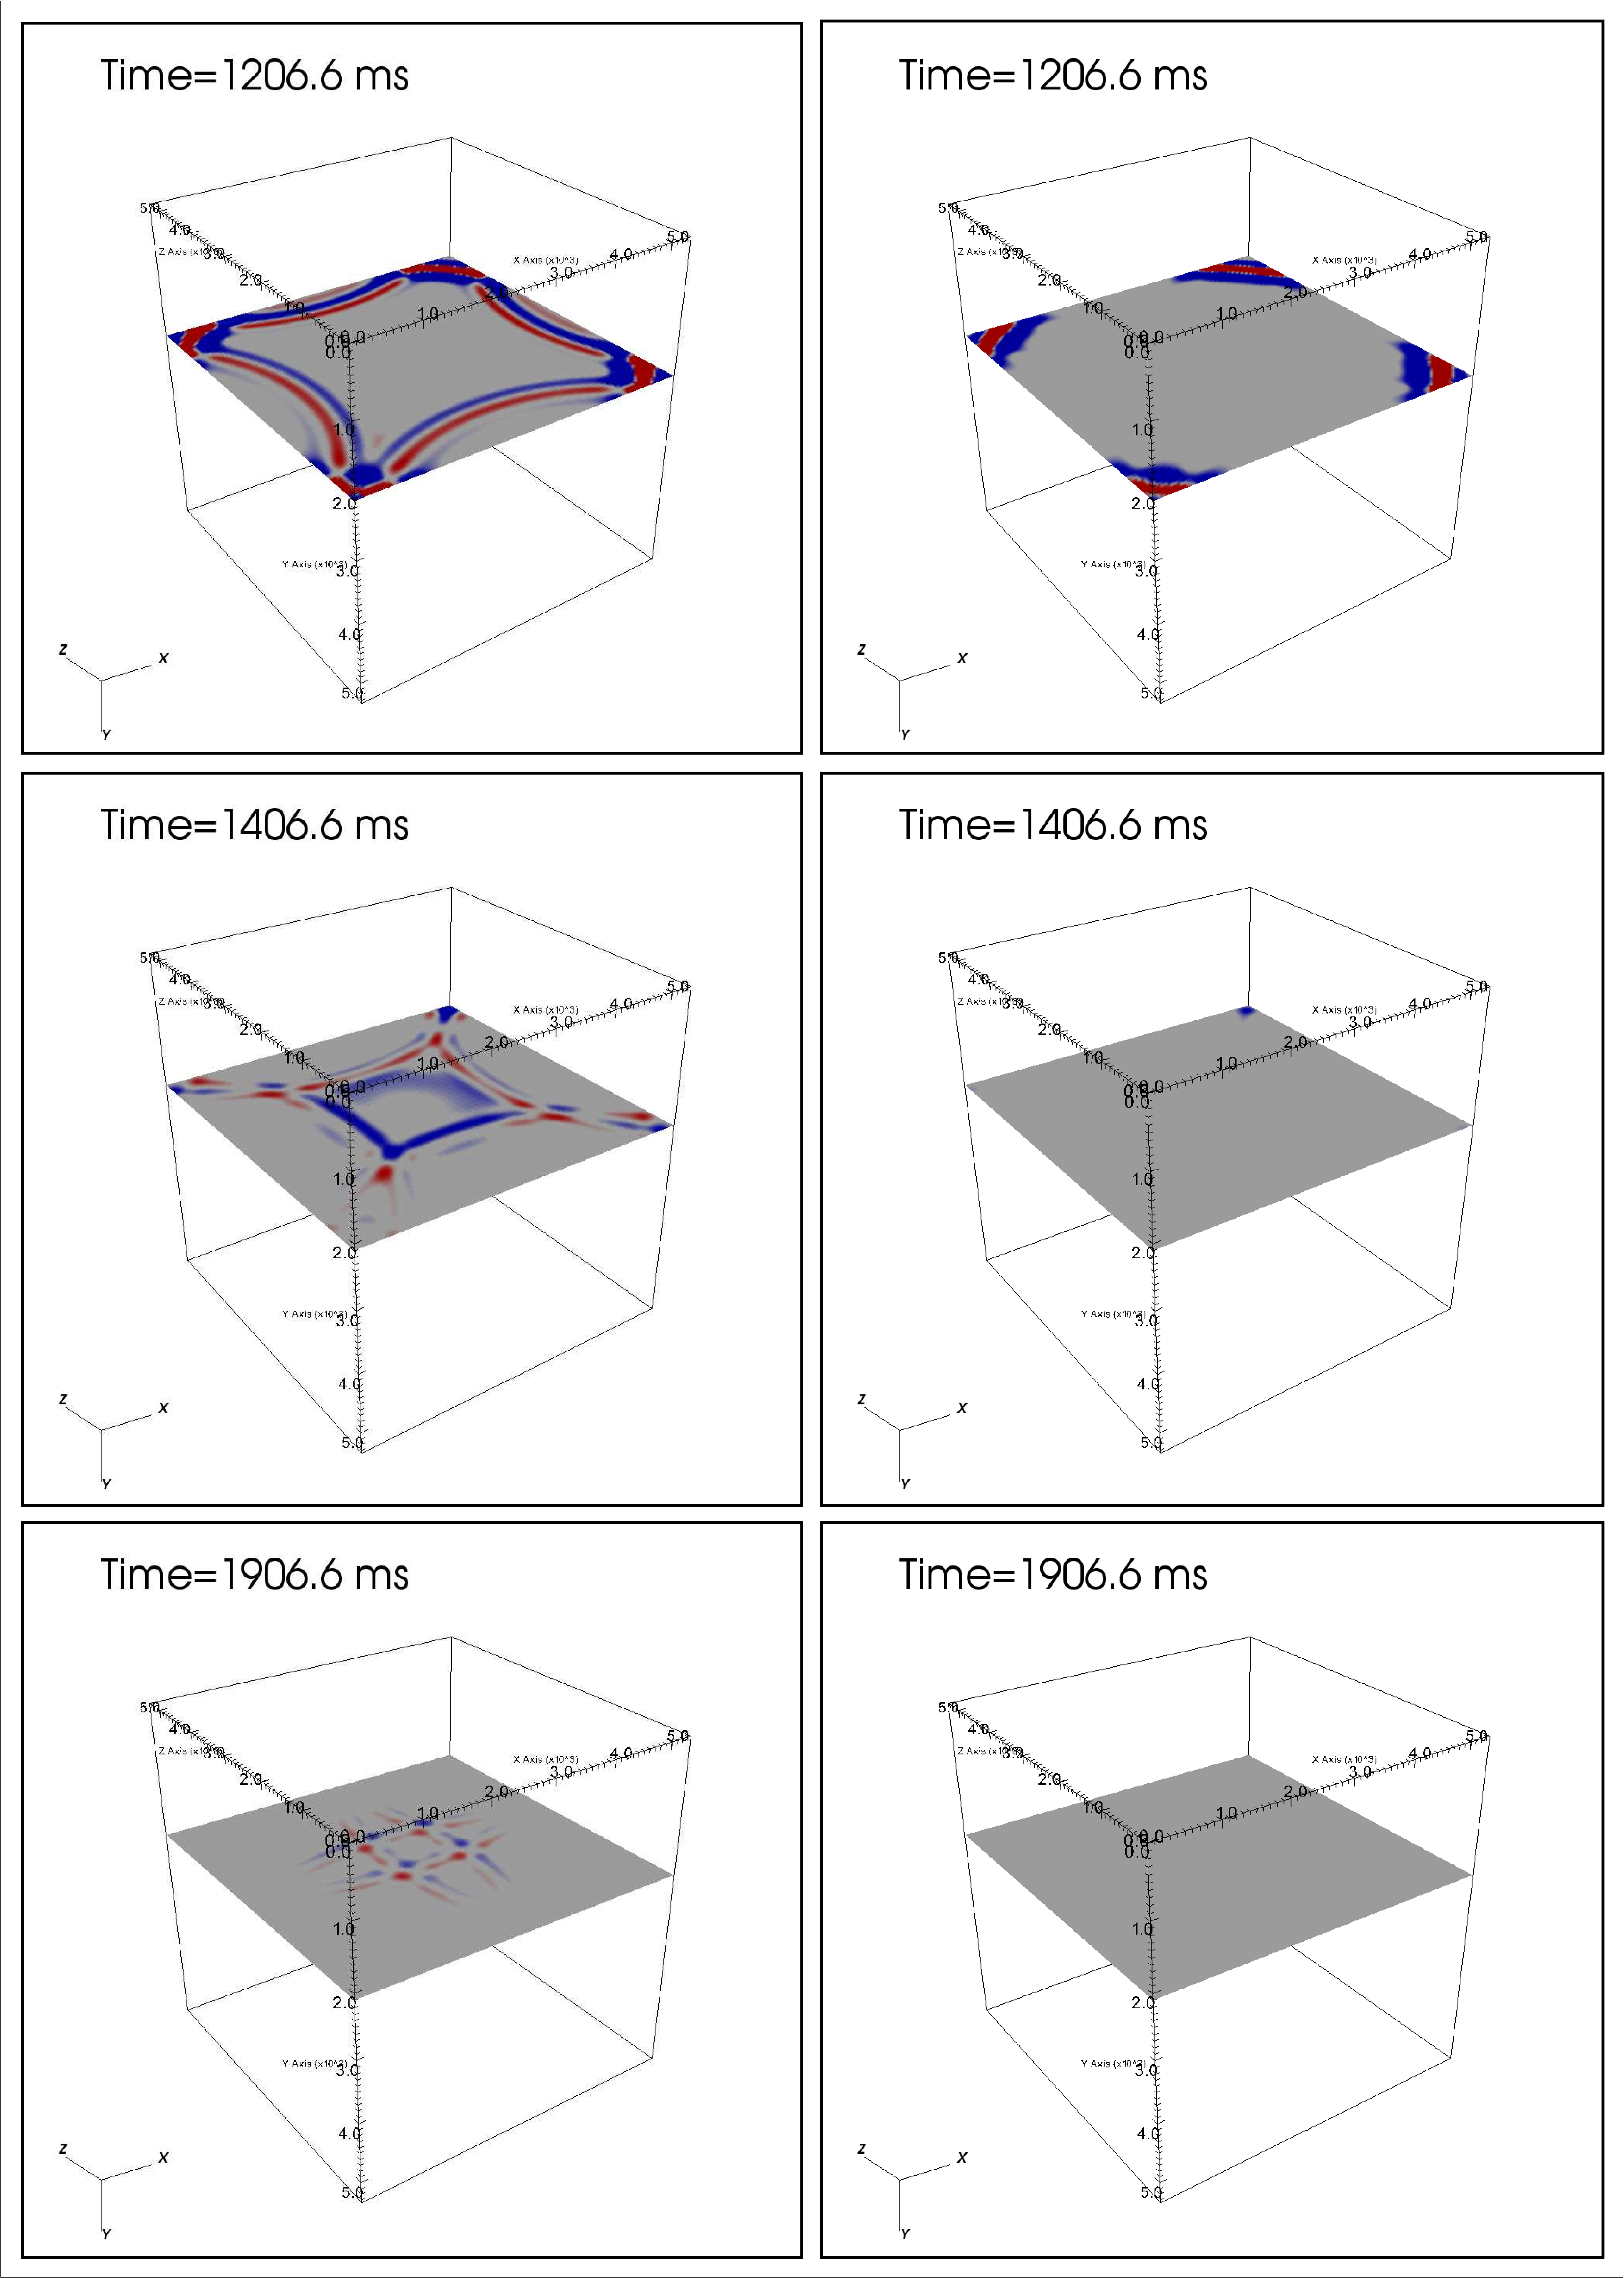
\includegraphics[width=13cm]{figures/ABS_PML_comp_shots.pdf}
\caption{\label{comp_EXP_PML} Comparison between exponential damping (left column) and PML (right column) absorbing boundary conditions for a homogeneous full space model.}
\end{center}
\end{figure} 
\end{enumerate} 
\clearpage
\section{Numerical Artefacts and Instabilities}\label{num_instab}
To avoid numerical artefacts and instabilities during a FD modelling run, spatial and temporal sampling conditions for the wavefield 
have to be satisfied. These will be discussed in the following two sections. 
\subsection{Grid Dispersion}\label{grid-dispersion}
The first question when building a FD model is: What is the maximum spatial grid point distance dh, for a correct sampling of the wavefield ? To answer this question we take a look at this simple example: The particle displacement in x-direction is defined by a sine function:
\EQ{grid_disp:1}{\rm{u_x=\sin\biggl(2 \pi \frac{x}{\lambda}\biggr),}}
where $\rm{\lambda}$ denotes the wavelength. When calculating the derivation of this function analytically at $\rm{x=0}$ and setting $\rm{\lambda=1\;m}$ we get:
\EQ{grid_disp:2}{\rm{\frac{d u_x}{d x}\biggl|_{x=0}=\frac{2 \pi}{\lambda} \cos\biggl(2 \pi \frac{x}{\lambda}\biggr)\biggl|_{x=0}=2 \pi.}}
In the next step the derivation is approximated numerically by a staggered 2nd order finite-difference operator:
\EQ{grid_disp:3}{\rm{\frac{d u_x}{d x}\biggl|_{x=0} \approx \frac{u_x(x+\frac{1}{2}\Delta x)-u_x(x-\frac{1}{2}\Delta x)}{\Delta x}\biggl|_{x=0}=\frac{\sin \biggl(\frac{2 \pi (x+\frac{1}{2}dx)}{\lambda} \biggr)-\sin \biggl(\frac{2 \pi (x-\frac{1}{2}dx)}{\lambda} \biggr)}{\Delta x}.}}
Using the Nyquist-Shannon sampling theorem it should be sufficient to sample the wavefield with $\rm{\Delta x = \lambda/2}$. In table \ref{grid_disp.1} the
numerical solutions of eq. \ER{grid_disp:3} and the analytical solution \ER{grid_disp:2} are compared for different sample intervals 
$\rm{\Delta x = \lambda /n}$, where n is the number of gridpoints per wavelength. For the case n=2, which corresponds to the Nyquist-Shannon theorem, the
numerical solution is $\rm{\frac{d u_x}{d x}|_{x=0}=4.0}$, which is not equal with the analytical solution $\rm{2 \pi}$. A refinement of the spatial
sampling of the wavefield results in an improvement of the finite difference solution. For $\rm{n=16}$ the numerical solution is accurate to the second
decimal place. The effect of a sparsly sampled pressure field is illustrated in \FIG{grid_disp_pics} for a homogeneous block model with stress free surfaces. The dimensions of the FD grid are fixed
and the central frequency of the source signal is increased systematically. 
When using a spatial sampling of 16 grid points per minimum wavelength (\FIG{grid_disp_pics}, top) the wavefronts are sharply defined. For $\rm{n=4}$ 
grid points a slight numerical dispersion of the wave occurs (\FIG{grid_disp_pics}, center). This effect is obvious when using the Nyquist criterion ($\rm{n=2}$) 
(\FIG{grid_disp_pics}, bottom). Since the numerical calculated wavefield seem to be dispersive this numerical artefact is called {\bf{grid dispersion}}. 
To avoid the occurence of grid dispersion the following criteria for the spatial grid spacing dh has to be satisfied:
\EQ{grid_disp:4}{\rm{dh \le \frac{\lambda_{min}}{n} = \frac{V_{min}}{n\; f_{max}}.}}
Here $\rm{\lambda_{min}}$ denotes the minimum wavelength, $\rm{V_{min}}$ the minimum velocity in the model and $\rm{f_{max}}$ is the maximum
frequency of the source signal.  
Depending on the accuracy of the used FD operator the parameter n is different.  In table \ref{grid_disp.2} n is listed for different FD operator lengths 
and types (Taylor and Holberg operators). The Holberg coefficients are calculated for a minimum dispersion error of $\rm{0.1\%}$ at $\rm{3 f_{max}}$. For short operators n should be choosen relatively large, so the spatial grid spacing is small, while for longer FD operators n is smaller and the grid spacing can be larger. 
\begin{table}[hbt]
\begin{center}
\begin{tabular}{ccc}\hline \hline
n &  $\rm{\Delta x\; [m]}$ & $\rm{\frac{d v_x}{d x}|_{x=0}\; []}$ \\ \hline 
analytical & - & $\rm{2\pi \approx 6.283}$ \\ 
2 & $\rm{\lambda/2}$ & 4.0 \\ 
4 & $\rm{\lambda/4}$ & 5.657 \\ 
8 & $\rm{\lambda/8}$ & 6.123 \\ 
16 & $\rm{\lambda/16}$ & 6.2429 \\ 
32 & $\rm{\lambda/32}$ & 6.2731\\ \hline \hline
\end{tabular}
\caption{\label{grid_disp.1} Comparison of the analytical solution Eq. \ER{grid_disp:2} with the numerical solution Eq. \ER{grid_disp:3} 
for different grid spacings $\rm{\Delta x = \lambda /n}$.}
\end{center}
\end{table}
 
\begin{table}[hbt]
\begin{center}
\begin{tabular}{ccc}\hline \hline
FDORDER & n (Taylor) & n (Holberg) \\ \hline 
2nd   &   12       &  12         \\
4th   &   8        &  8.32       \\
6th   &   6        &  4.77       \\
8th   &   5        &  3.69       \\ 
10th  &   5        &  3.19       \\
12th  &   4        &  2.91       \\
\hline \hline
\end{tabular}
\caption{\label{grid_disp.2} The number of grid points per minimum wavelength n for different orders (2nd-12th) and types (Taylor and
Holberg) of FD operators. For the Holberg coefficients n is calculated for a minimum dispersion error of $\rm{0.1\%}$ at $\rm{3 f_{max}}$.}
\end{center}
\end{table} 
\clearpage
\begin{figure}[ht]
\begin{center}
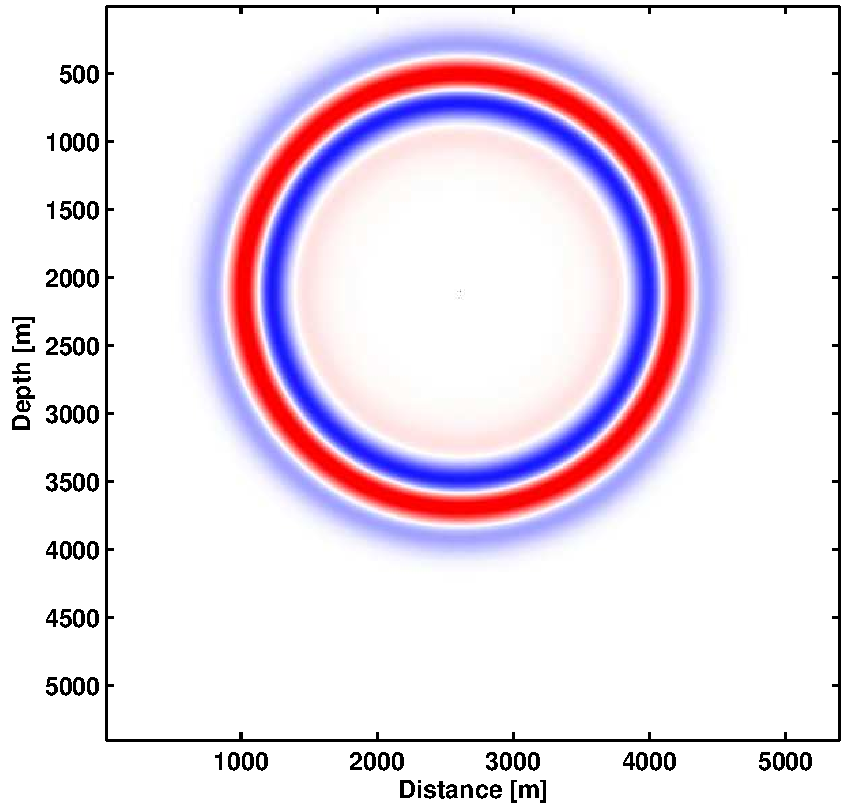
\epsfig{file=figures/homogenous_grid_n_16_5.pdf, width=6 cm}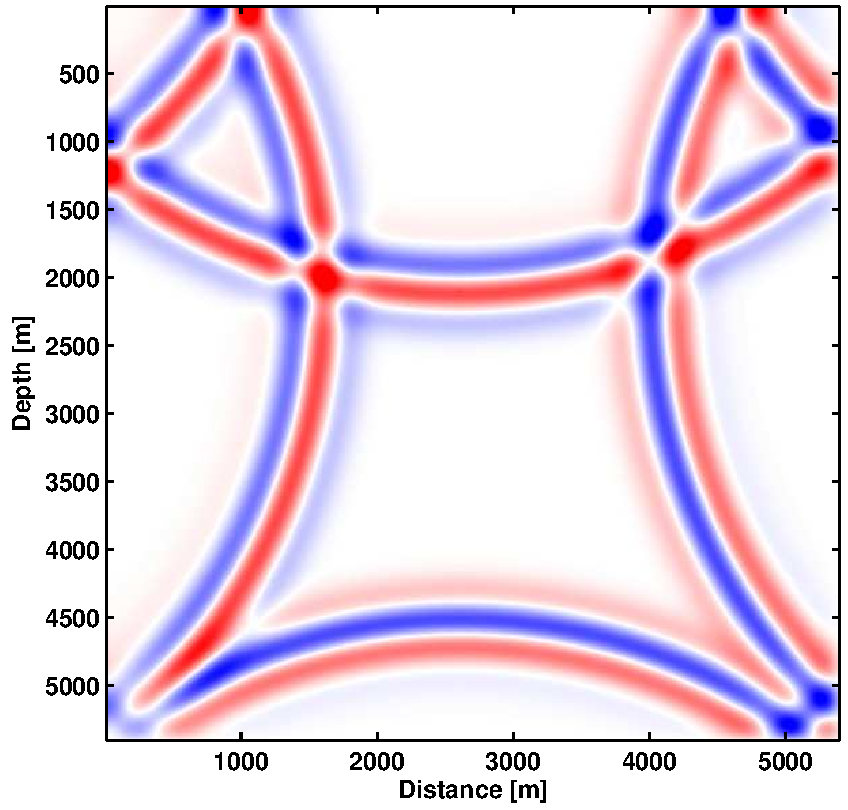
\epsfig{file=figures/homogenous_grid_n_16_10.pdf, width=6 cm}
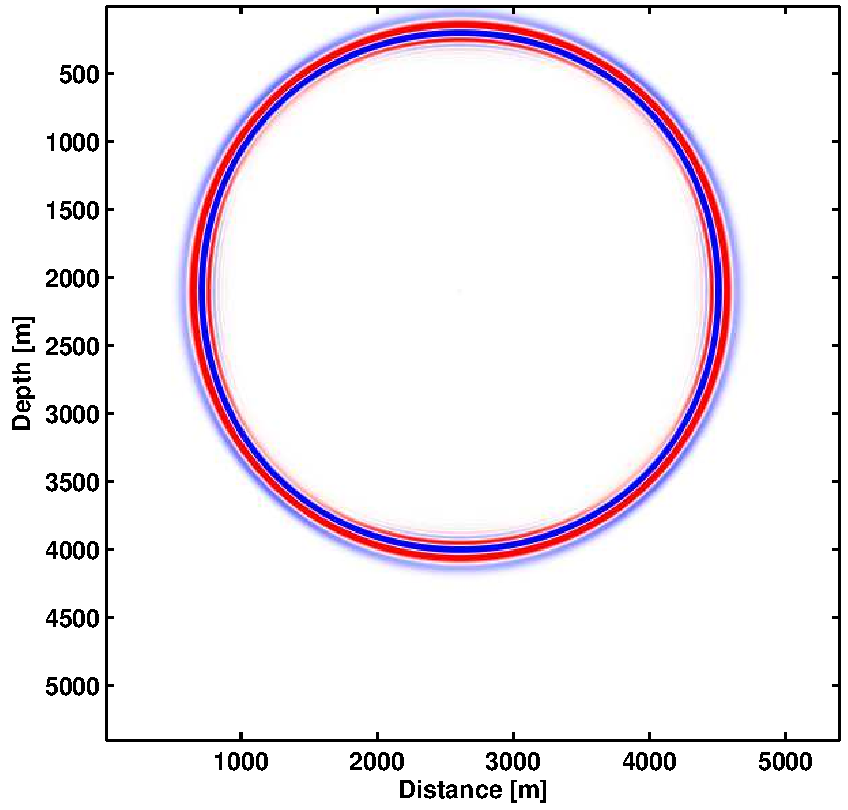
\epsfig{file=figures/homogenous_grid_n_4_5.pdf, width=6 cm}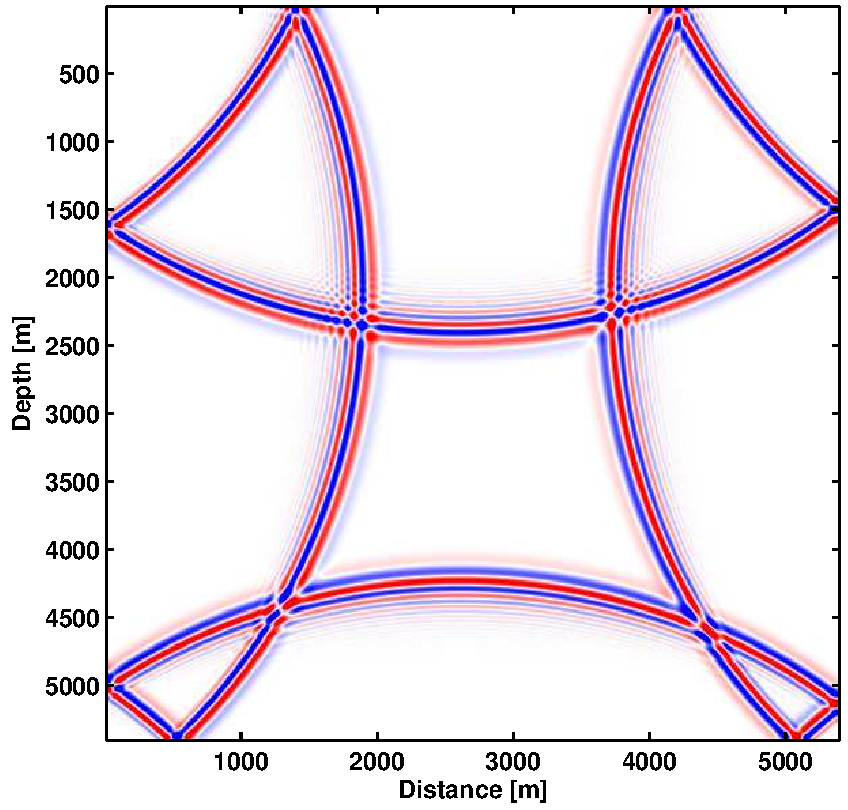
\epsfig{file=figures/homogenous_grid_n_4_10.pdf, width=6 cm}
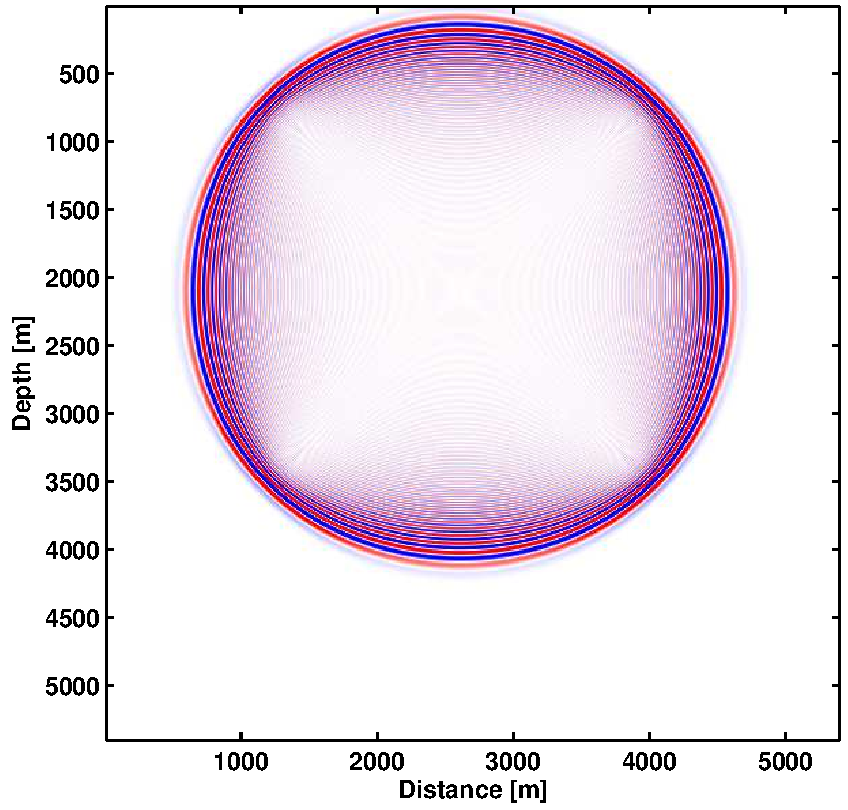
\epsfig{file=figures/homogenous_grid_n_2_5.pdf, width=6 cm}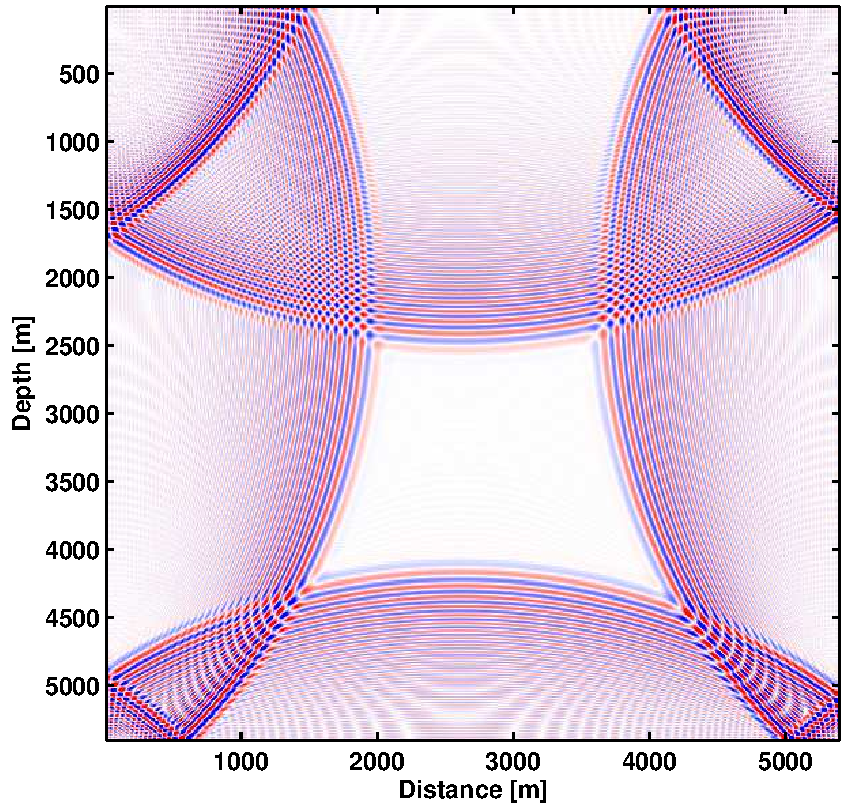
\epsfig{file=figures/homogenous_grid_n_2_10.pdf, width=6 cm}
\caption{\label{grid_disp_pics} The influence of grid dispersion in FD modeling: Spatial sampling of the wavefield using n=16 (top), n=4 (center) and n=2 gridpoints (bottom) per minimum wavelength $\rm{\lambda_{min}}$.}
\end{center}
\end{figure}
\clearpage
\subsection{The Courant Instability}\label{courandt}
Beside the spatial, the temporal discretization has to satisfy a sampling criterion to ensure the stability of the FD code. If a 
wave is propagating on a discrete grid, then the timestep $\rm{dt}$ has to be less than the time for the wave to travel between two adjacent grid 
points with grid spacing $\rm{dh}$. For an elastic 2D grid this means mathematically:
\EQ{courandt:1}{\rm{dt \le \frac{dh}{h \sqrt{2} V_{max}},}}
where $\rm{V_{max}}$ is the maximum velocity in the model. The factor h depends on the order of the FD operator and can easily calculated by summing over the weighting coefficients $\rm{\beta_i}$
\EQ{courant:1:1}{\rm{h = \sum_i \beta_i.}}
In table \ref{courant.1} h is listed for different FD operator lengths and types (Taylor and Holberg operators). Criterion \ER{courandt:1} 
is called {\bf{Courant-Friedrichs-Lewy criterion}} (\cite{courant:28}, \cite{courant:67}). \FIG{courandt_pics} shows the evolution of the pressure field when the Courant criterion is violated. After a few time steps the amplitudes are growing to infinity and the calculation becomes unstable.
\begin{table}[hbt]
\begin{center}
\begin{tabular}{ccc}\hline \hline
FDORDER & h (Taylor)      & h (Holberg) \\ \hline 
2nd   &   1.0             &  1.0        \\
4th   &   7/6             &  1.184614   \\
6th   &   149/120         &  1.283482   \\
8th   &   2161/1680       &  1.345927   \\
10th  &   53089/40320     &  1.387660   \\
12th  &   1187803/887040  &  1.417065   \\   
\hline \hline
\end{tabular}
\caption{\label{courant.1} The factor h in the Courant criterion for different orders (2nd-12th) and types (Taylor and Holberg) of FD operators.}
\end{center}
\end{table} 
\clearpage
\begin{figure}[ht]
\begin{center}
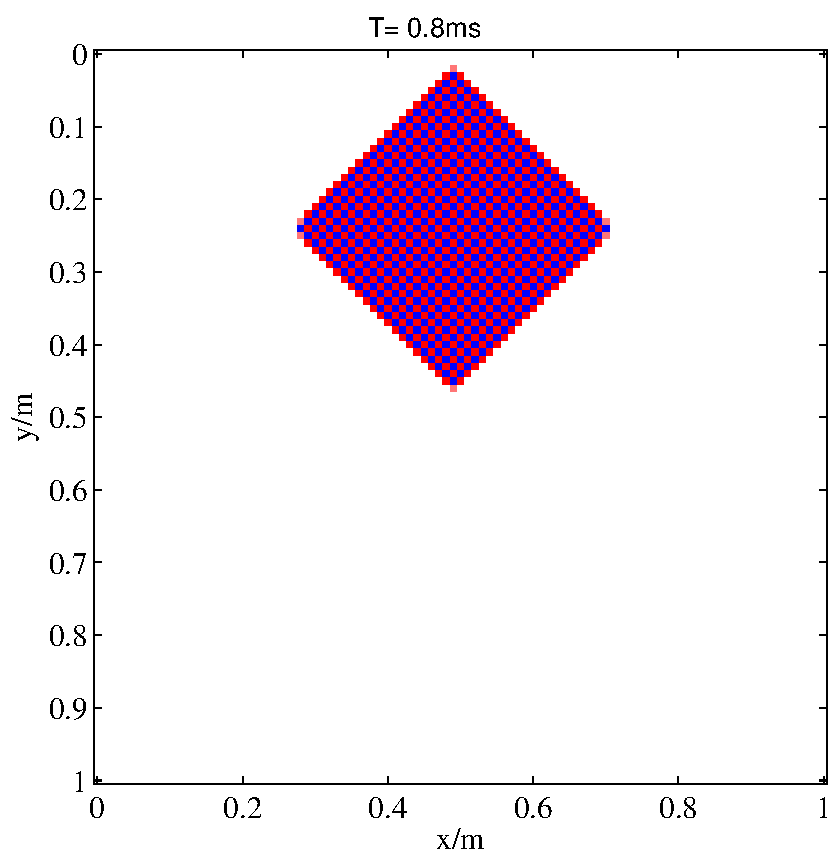
\epsfig{file=figures/courandt_1.pdf, width=7 cm}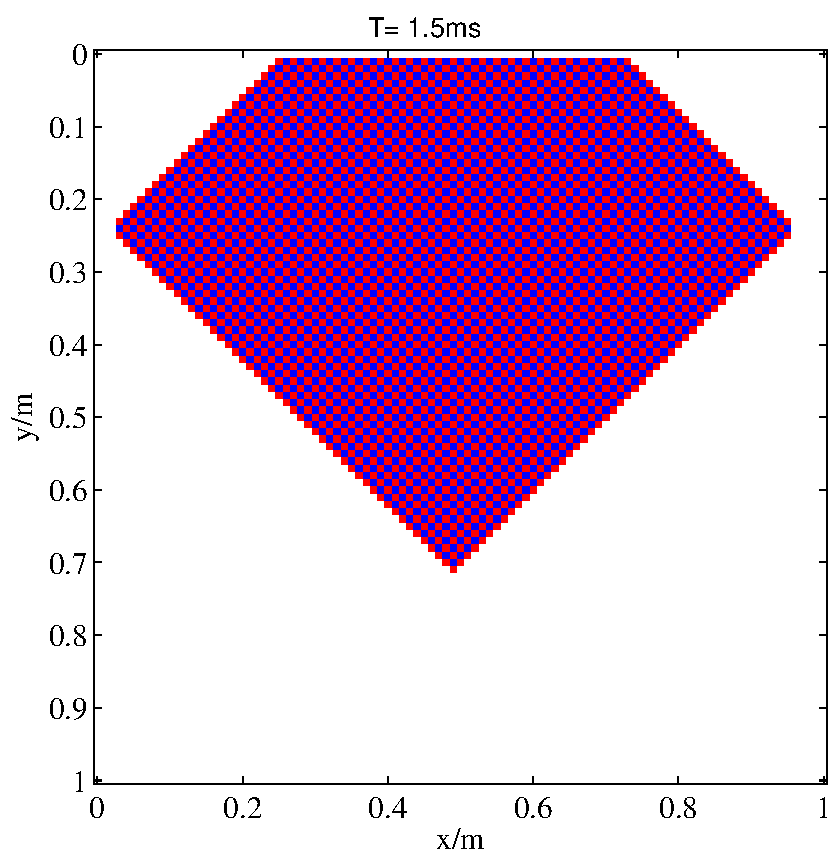
\epsfig{file=figures/courandt_2.pdf, width=7 cm}
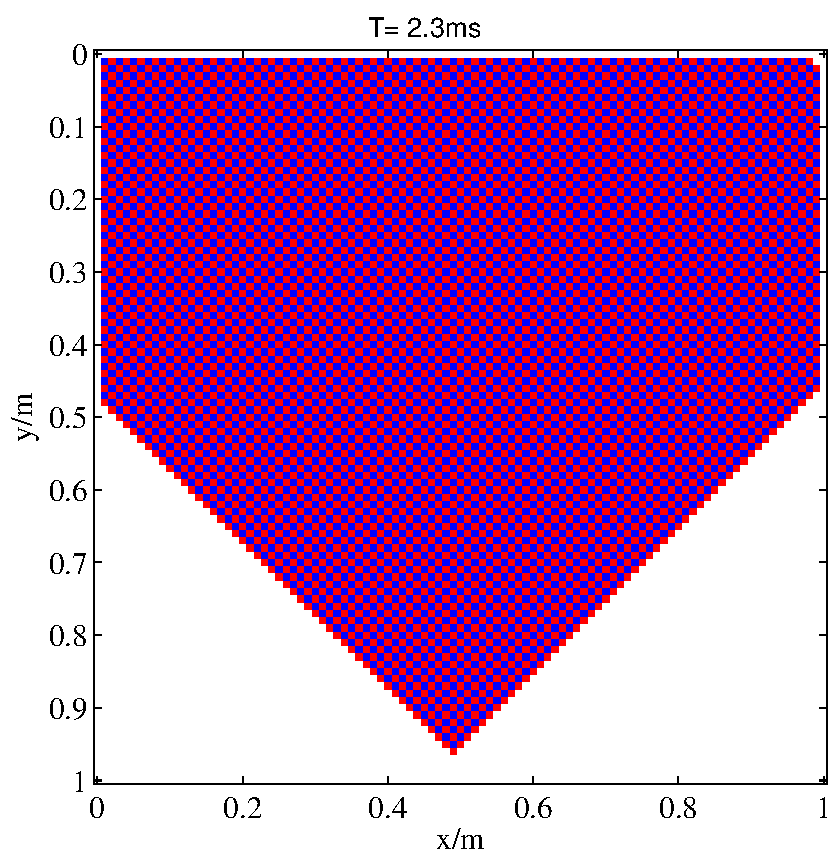
\epsfig{file=figures/courandt_3.pdf, width=7 cm}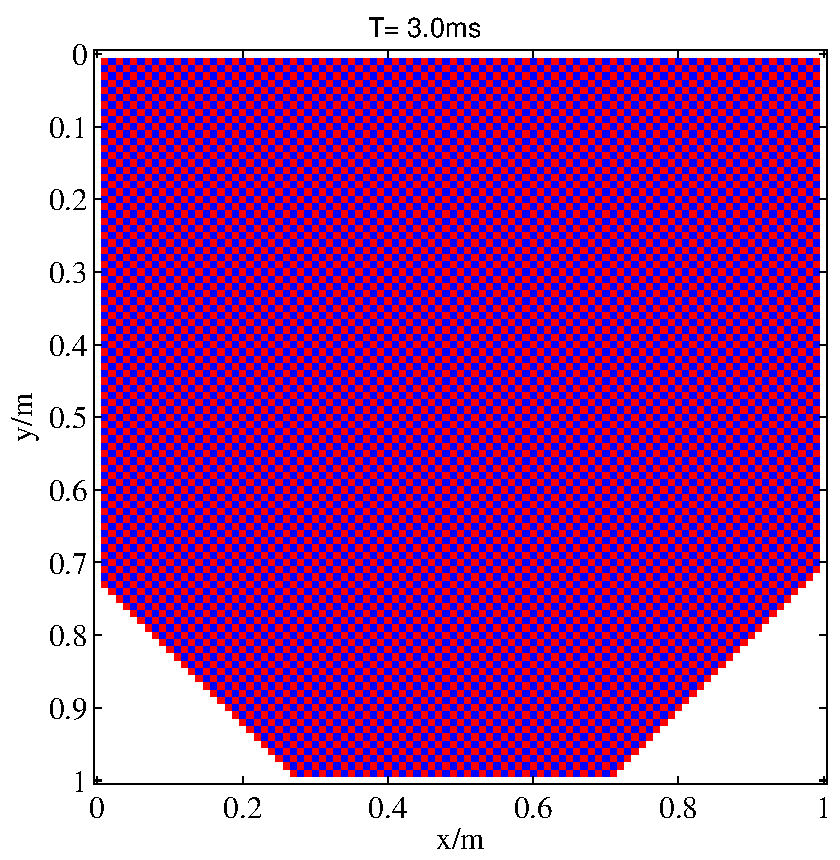
\epsfig{file=figures/courandt_4.pdf, width=7 cm}
\caption{\label{courandt_pics} Temporal evolution of the Courant instability. In the colored areas the wave amplitudes are extremly large.}
\end{center}
\end{figure}
\clearpage


% ------------------------------------
\chapter{The adjoint problem}
% ------------------------------------

The aim of full waveform tomography is to find an ''optimum'' model which can explain the data very well. It should not only explain the 
first arrivals of specific phases of the seismic wavefield like refractions or reflections, but also the amplitudes which contain information 
on the distribution of the elastic material parameters in the underground. To achieve this goal three problems have to be solved:
\begin{enumerate}
\item What is an ''optimum'' model ?
\item How can this model be found ?
\item Is this model unique or are other models existing, which could explain the data equally well ?   
\end{enumerate}
\section{What is an ''optimum'' model ?}
In reflection seismics the $\rm{i^{th}}$ component of the elastic displacement field $\rm{u_i(\mathbf{x_s},\mathbf{x_r},t)}$ 
excited by sources located at $\rm{\mathbf{x_s}}$ will be recorded by receivers at $\rm{\mathbf{x_r}}$ at time t. 
For a given distribution of the material parameters the forward problem Eq. \ref{2:20} can be solved by finite differences (section \ref{elastic_FD_Code}). The result is a model data set $\rm{\mathbf{u^{mod}}}$. This modelled data can be compared with the field data $\rm{\mathbf{u^{obs}}}$. If the misfit or data residuals $\rm{\delta \mathbf{u} = \mathbf{u^{mod}} - \mathbf{u^{obs}}}$ (\FIG{sketch_data_res}) between the modelled and the field data is small the model can explain the data very well. If the residuals are large the model cannot explain the data. The misfit can be measured by a vector norm $\rm{|L|_p}$ which is defined for $\rm{p=1,2,...}$ as  
\begin{equation} 
\rm{|L|_p = \biggl(\sum_i|\delta u_i|^p\biggr)^{1/p}} 
\end{equation} 
The special case $\rm{|L|_\infty}$ is defined as
\begin{equation} 
\rm{|L|_\infty = max_i|\delta u_i|^p} 
\label{l-infty}
\end{equation} 
The L2-norm 
\begin{equation} 
\rm{E=|L|_2 = \frac{1}{2}\mathbf{\delta u^T} \mathbf{\delta u}} 
\label{l-norm}
\end{equation} 
has a special physical meaning. It represents the residual elastic energy contained in the data residuals $\rm{\delta \mathbf{u}}$. An optimum model can be found in a minimum of the residual energy. Therefore the optimum model is the solution of a nonlinear optimization problem.
\begin{figure}[!bh]
\begin{center}
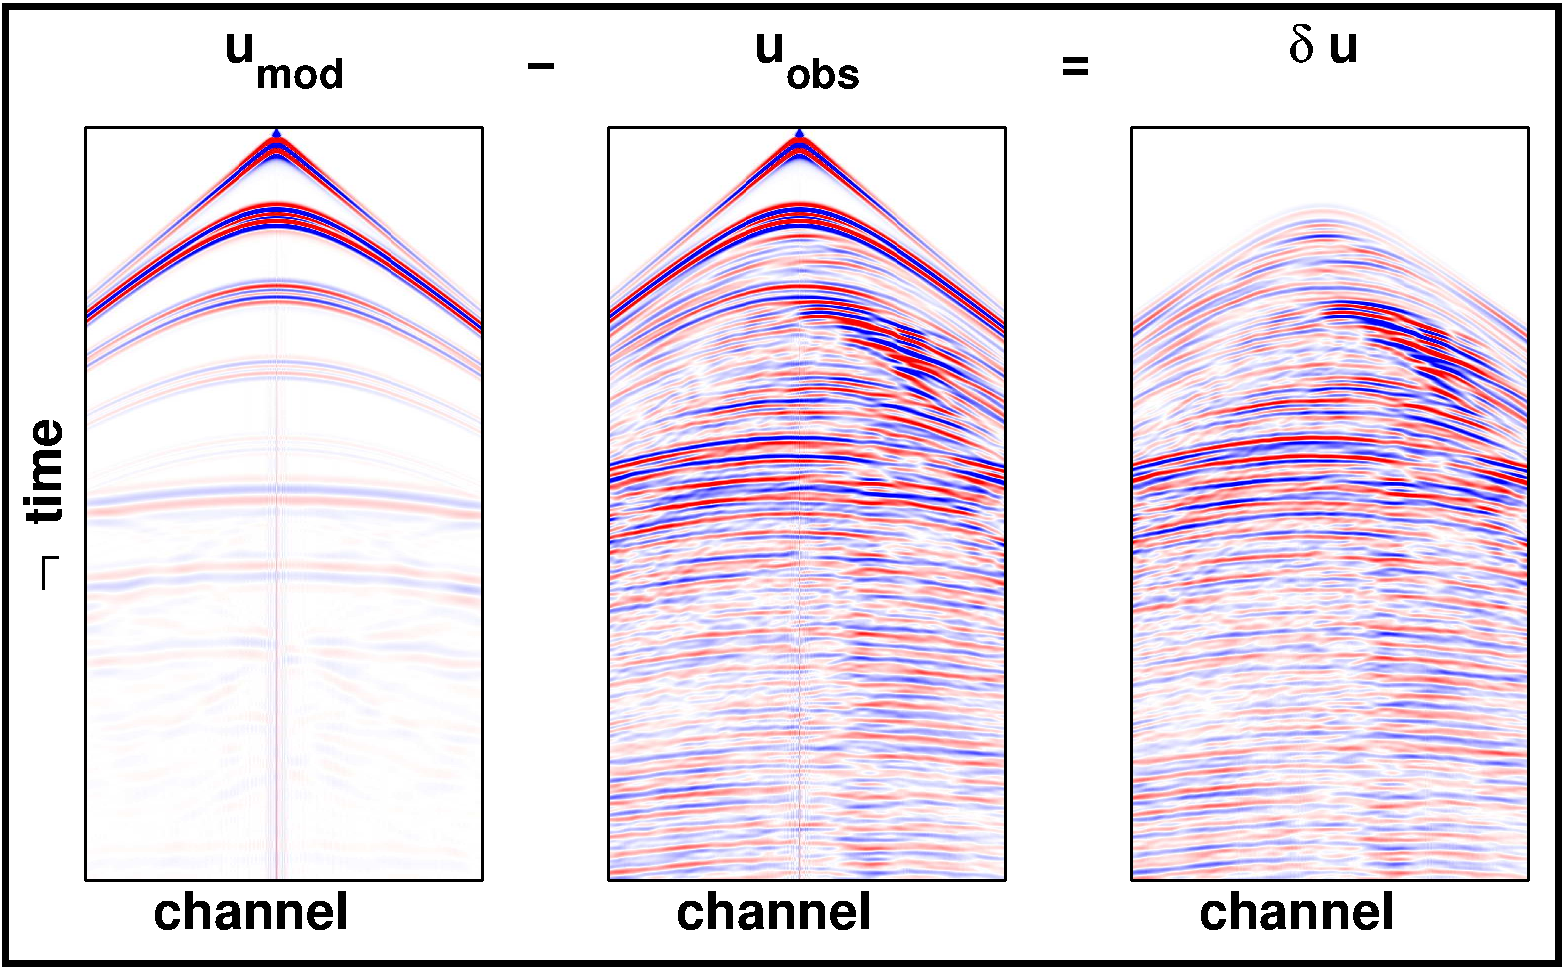
\includegraphics[width=15 cm]{figures/data_res_sketch_1.pdf}
\caption{Definition of data residuals $\rm{\mathbf{\delta u}}$.}
\label{sketch_data_res}
\end{center}
\end{figure} 
\newpage
\section{How to find an optimum model}
Figure \ref{sketch_grad} shows a schematic sketch of the residual energy at one point in space as a function of two model parameters 
$\rm{\lambda}$ and $\rm{\mu}$. The colors represent different values of the residual energy. Red areas represent models with high residual 
energy which do not fit the data, while the blue parts are good fitting models with low residual energies. The aim is to find the minimum of 
the residual energy marked by the red cross. Starting at a point $\rm{\mathbf{m_1} = (\lambda_1 (\mathbf{x}), \mu_1 (\mathbf{x}), \rho_1 (\mathbf{x}),)}$ in the parameter space we want to find the minimum by updating the material parameters in an iterative way
\begin{equation} 
\rm{\mathbf{m}_{2} = \mathbf{m}_{1} + \mu_1 \mathbf{\delta m}_{1}, }
\label{eq_update}
\end{equation}
along the search direction $\rm{\mathbf{\delta m}_{1}}$ with the step length $\rm{\mu_1}$. 
\begin{figure}[!bh]
\begin{center}
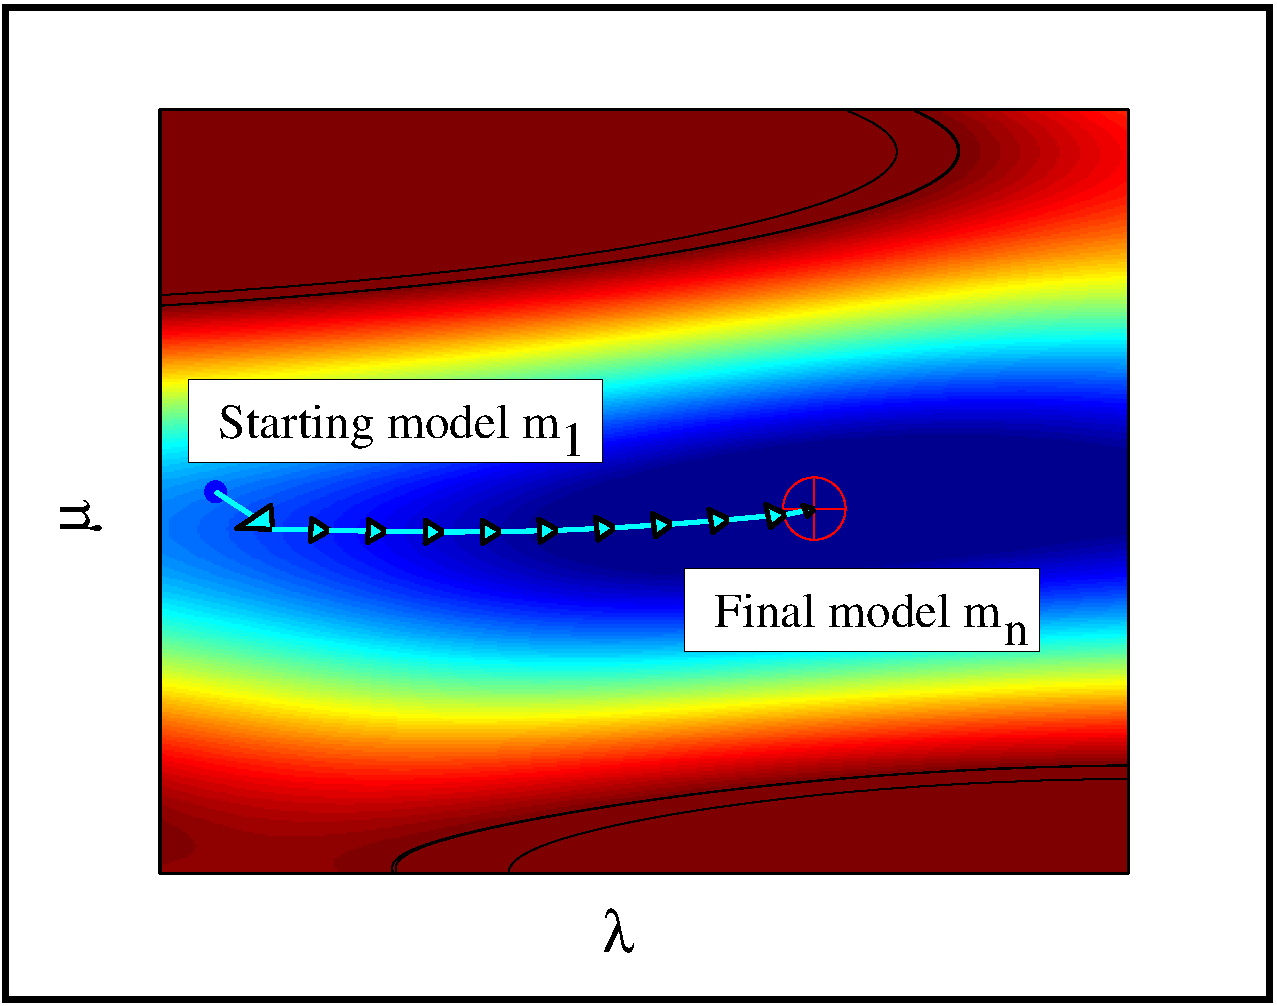
\includegraphics[width=12.5cm]{figures/sketch_grad_1.pdf}
\caption{Schematic sketch of the residual energy at one point in space as a function of two model parameters $\rm{m_1}$ and $\rm{m_2}$. The blue dot denotes the starting point in the parameter space, while the red cross marks a minimum of the objective function.}
\label{sketch_grad}
\end{center}
\end{figure} 
To find the optimum search direction $\rm{\mathbf{\delta m}_{1}}$ we expand the residual energy $\rm{E(\mathbf{m}_{1} + \mathbf{\delta m}_{1})}$ near the starting point in a Taylor series:
\begin{equation}
\rm{E(\mathbf{m}_{1} + \mathbf{\delta m}_{1}) \approx E(\mathbf{m}_{1}) + \mathbf{\delta m}_{1} \biggl(\frac{\partial E}{\partial m}\biggr)_1 + \frac{1}{2} \mathbf{\delta m}_{1} \biggl(\frac{\partial^2 E}{\partial m^2}\biggr)_1 \mathbf{\delta m}_{1}^T}   
\label{eq_update_taylor}
\end{equation} 
and set the derivative of Eq. \ref{eq_update_taylor} with respect to $\rm{\delta \mathbf{m_1}}$ zero
\begin{equation}
\rm{\frac{\partial E(\mathbf{m}_{1} + \mathbf{\delta m}_{1})}{\partial \mathbf{\delta m}_{1}} = \biggl(\frac{\partial E}{\partial m}\biggr)_1 + \mathbf{\delta m}_{1} \biggl(\frac{\partial^2 E}{\partial m^2}\biggr)_1 = 0}   
\label{eq_update_taylor_prime}
\end{equation} 
Which finally leads to
\begin{equation}
\rm{\mathbf{\delta m}_{1} = - \biggl(\frac{\partial^2 E}{\partial m^2}\biggr)_1^{-1} \biggl(\frac{\partial E}{\partial m}\biggr)_1 = -  \mathbf{H_1}^{-1} \biggl(\frac{\partial E}{\partial m}\biggr)_1}   
\label{eq_opt_search}
\end{equation} 
where $\rm{(\partial E/\partial \mathbf{m})_1}$ denotes the steepest-descent direction of the objective function and $\rm{\mathbf{H_1}^{-1}}$ the inverse Hessian matrix. The inverse Hessian matrix for the elastic problem is often singular and can only be calculated with high computational costs. Therefore the inverse Hessian matrix is approximated by a preconditioning operator P. There is no general rule for an optimum preconditioning operator. 
\begin{equation}
\rm{\mathbf{\delta m}_{1} \approx - \mathbf{P_1} \biggl(\frac{\partial E}{\partial m}\biggr)_1.}   
\label{eq_opt_search1}
\end{equation} 
By replacing $\rm{\mathbf{\delta m}_{1}}$ in Eq. \ref{eq_update} with Eq. \ref{eq_opt_search1} we get         
\begin{equation} 
\rm{\mathbf{m}_{2} = \mathbf{m}_{1} - \mu_1 \mathbf{P_1} \biggl(\frac{\partial E}{\partial \mathbf{m}}\biggr)_1, }
\label{eq_update1}
\end{equation} 
The optimum model parameters can be found along the negative gradient direction of the residual energy. The starting point $\rm{\mathbf{m_1}}$ is not a particular point, so the update function can be applied to every point in the parameter space $\rm{\mathbf{m_n}}$ 
\begin{equation} 
\rm{\mathbf{m}_{n+1} = \mathbf{m}_{n} - \mu_n \mathbf{P_n} \biggl(\frac{\partial E}{\partial \mathbf{m}}\biggr)_n. }
\label{eq_updatefinal}
\end{equation} 

\section{Calculation of the gradient direction}% $\rm{\frac{\partial E}{\partial \mathbf{m}}}$}
To estimate the gradient direction $\rm{\partial E/\partial \mathbf{m}}$ the residual energy is rewritten as:
\begin{equation} 
\rm{E = \frac{1}{2}\mathbf{\delta u^T} \mathbf{\delta u} = \frac{1}{2} \sum_{sources} \int dt \sum_{receiver} \mathbf{\delta u}^2(x_r, x_s, t) } 
\label{L2_continous}
\end{equation}
After derivation with respect to a model parameter $\rm{\mathbf{m}}$ we get
\begin{equation} 
\begin{split}
\rm{\frac{\partial E}{\partial \mathbf{m}}} &\rm{= \sum_{sources} \int dt \sum_{receiver} \frac{\partial \mathbf{\delta u}}{\partial
\mathbf{m}} \mathbf{\delta u}}\\ 
& \rm{= \sum_{sources} \int dt \sum_{receiver} \frac{\partial {(\mathbf{u^{mod}\mathbf(m)} - \mathbf{u^{obs}})}}{\partial
\mathbf{m}}  \mathbf{\delta u} }\\ 
&\rm{= \sum_{sources} \int dt \sum_{receiver} \frac{\partial {\mathbf{u^{mod}(\mathbf{m})}}}{\partial \mathbf{m}}  \mathbf{\delta u}} 
\label{dL2_dm}
\end{split}
\end{equation}
Eq. \ER{dL2_dm} can be related to the mapping of small changes from the data to the model space and vice versa (\FIG{mapping_data_model}). 
\begin{figure}[ht]
\begin{center}
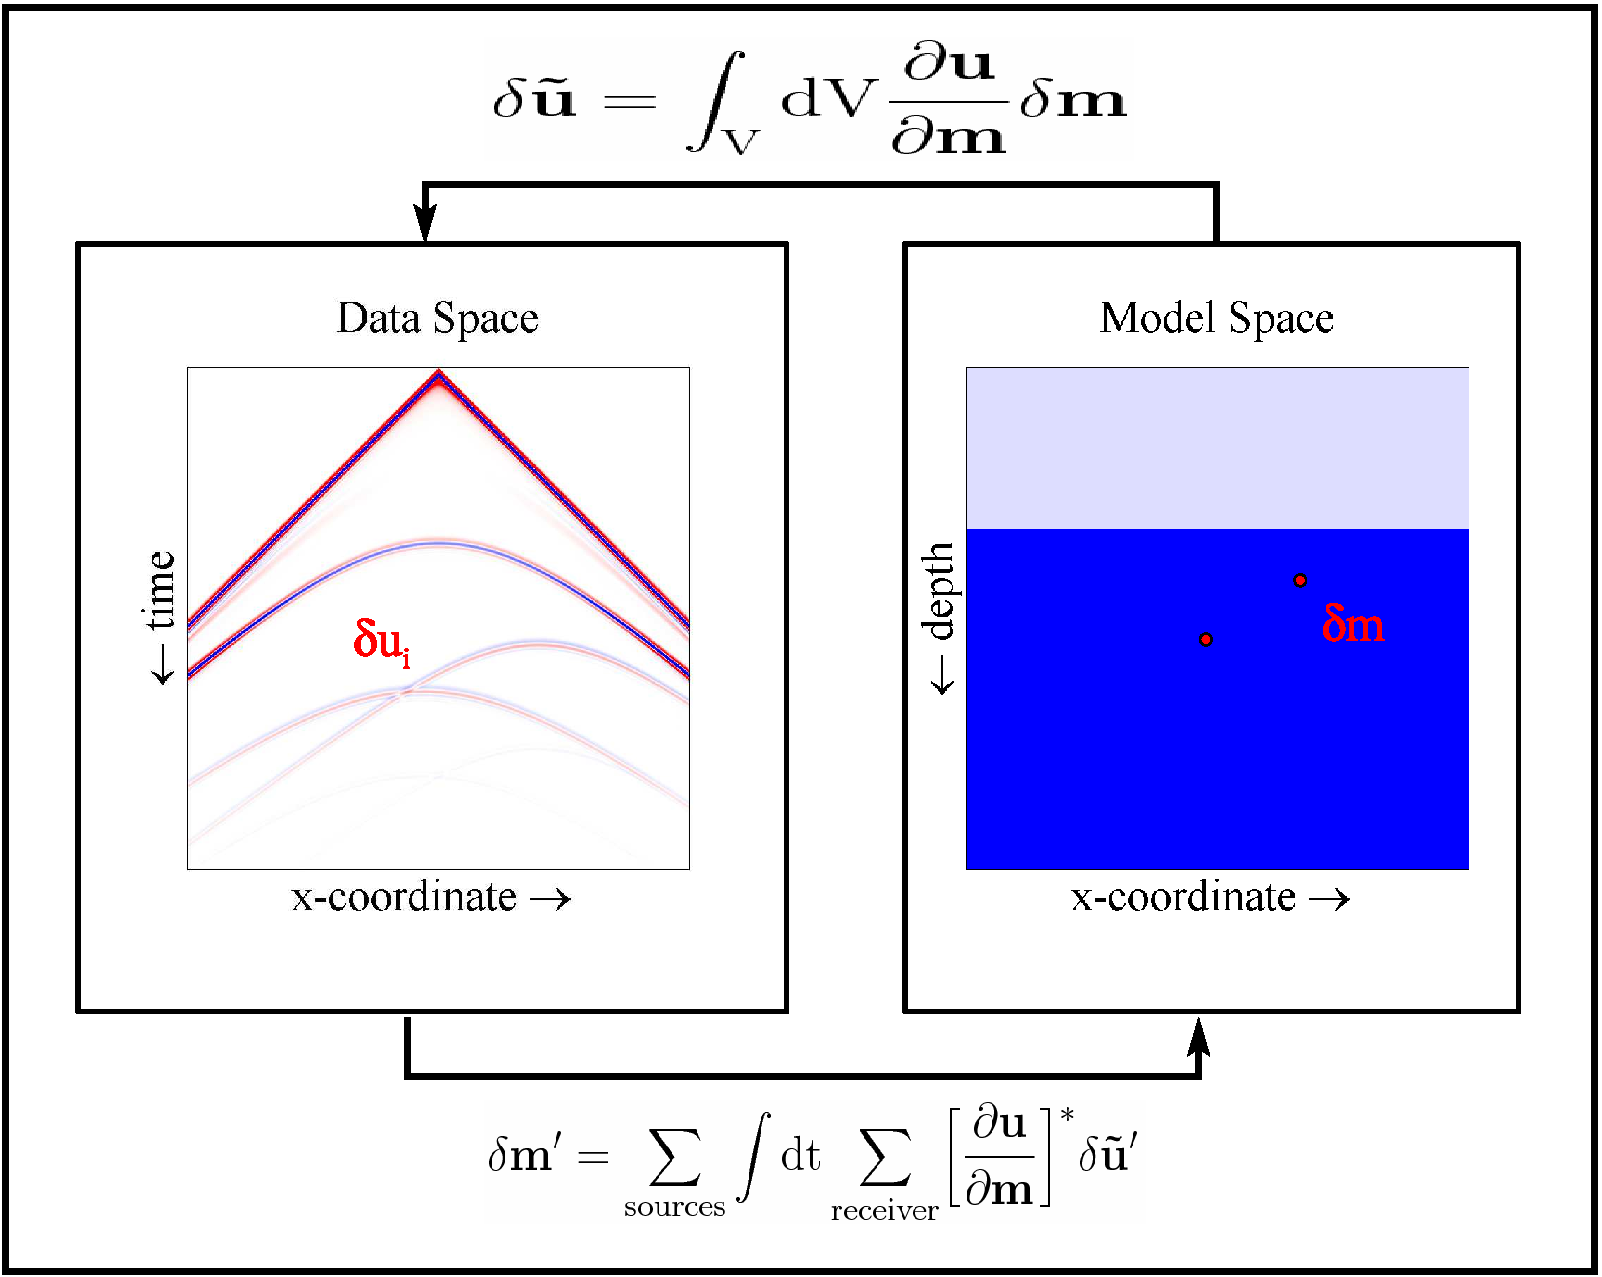
\includegraphics[width=10cm]{figures/mapping_data_model.pdf}
\caption{Mapping between model and data space and vice versa.}
\label{mapping_data_model}
\end{center}
\end{figure}
A small change in the model space $\rm{\delta \mathbf{m}}$, e.g. one model parameter at one point in space, will result in a small 
perturbation of the data space $\rm{\delta \mathbf{\tilde{u}}}$, e.g. one wiggle in the seismic section. If the Frech$\rm{\acute{e}}$t derivative $\rm{\frac{\partial \mathbf{u}}{\partial \mathbf{m}}}$ is known, all 
the small perturbations in model space can be integrated over the model volume V to calculate the total change in data space
(\cite{tarantola:2005}):
\begin{equation}
\rm{\delta \mathbf{\tilde{u}}(\mathbf{x_s},\mathbf{x_r},t) = \int_V dV \frac{\partial \mathbf{u}}{\partial \mathbf{m}} \delta 
\mathbf{m},}
\label{2:4}
\end{equation} 
or by introducing the linear operator $\rm{\hat{L}}$
\begin{equation}
\rm{\delta \mathbf{\tilde{u}} = \hat{L} \delta \mathbf{m} := \int_V dV \frac{\partial \mathbf{u}}{\partial \mathbf{m}} \delta 
\mathbf{m}.\notag}
\label{2:4:1}
\end{equation} 
In a similar way small changes in the data space $\rm{\delta \mathbf{\tilde{u}}'}$ can be integrated to calculate the total change in the model 
space $\rm{\delta \mathbf{m}'}$ (\cite{tarantola:2005})
\begin{equation}
\rm{\delta \mathbf{m'} =  \sum_{sources} \int dt \sum_{receiver} \biggl[\frac{\partial \mathbf{u}}{\partial \mathbf{m}}\biggr]^* \delta
\mathbf{\tilde{u}}',}
\label{3:6}
\end{equation}
or as operator equation
\begin{equation}
\rm{\delta \mathbf{m'} = \hat{L}^* \delta \mathbf{\tilde{u}}'. \notag}
\label{3:6:1}
\end{equation}
In this case the Frech$\rm{\acute{e}}$t derivative $\rm{\frac{\partial \mathbf{u}}{\partial \mathbf{m}}}$ is replaced by it's adjoint 
counterpart $\rm{\frac{\partial \mathbf{u}}{\partial \mathbf{m}}^*}$. Note that $\rm{\delta
\mathbf{\tilde{u}} \ne \delta \mathbf{\tilde{u}}'}$ and $\rm{\delta \mathbf{m} \ne \delta \mathbf{m}'}$, so there is no unique way to map perturbations from the model to the data space or vice versa. Because the operator $\rm{\hat{L}}$ is linear, the kernel of $\rm{\hat{L}}$ and it's adjoint counterpart $\rm{\hat{L}^*}$ are identical (see chapter 5.4.2 in \cite{tarantola:2005})
\begin{equation}
\rm{\biggl[\frac{\partial \mathbf{u}}{\partial \mathbf{m}}\biggr]^* = \biggl[\frac{\partial \mathbf{u}}{\partial \mathbf{m}}\biggr]} \notag
\end{equation}
Therefore the mapping from the data to the model space Eq. \ER{3:6} is equal to the gradient of the residual energy Eq. \ER{dL2_dm}: 

\begin{equation}
\begin{split}
\rm{\delta \mathbf{m'}} &\rm{=  \sum_{sources} \int dt \sum_{receiver} \biggl[\frac{\partial \mathbf{u_i}}{\partial \mathbf{m}}\biggr]^*
\delta \mathbf{\tilde{u}}'} \\
                   &\rm{=  \sum_{sources} \int dt \sum_{receiver} \biggl[\frac{\partial \mathbf{u_i}}{\partial \mathbf{m}}\biggr] \delta \mathbf{u}} \\
                   &\rm{=  \frac{\partial E}{\partial \mathbf{m}}}
\end{split}
\label{dm_dE_dm}
\end{equation}
if the perturbation of the data space $\rm{\delta \mathbf{\tilde{u}}'}$ is interpretated as data residuals $\rm{\delta \mathbf{u}}$. So the approach to estimate the gradient direction $\rm{\partial E/\partial m}$ can be split into 3 parts
\begin{enumerate}
\item Find a solution to the forward problem
\begin{equation}
\rm{\delta \mathbf{u} = \hat{L} \delta \mathbf{m}.\notag}
\end{equation} 
\item Identify the Frech$\rm{\acute{e}}$t kernels $\rm{\partial \mathbf{u}/\partial \mathbf{m}}$ 
\item Use the property, that a linear operator $\rm{\hat{L}}$ and it's adjoint $\rm{\hat{L}^*}$ have the same kernels and calculate the gradient direction by using:
\begin{equation}
\rm{\frac{\partial E}{\partial \mathbf{m}} = \delta \mathbf{m'} = \hat{L}^* \delta \mathbf{u}'. \notag}
\end{equation} 
\end{enumerate}
This is a very general approach. Now we apply this approach to the equations of motion for an elastic medium. The following derivation is much easier, when assuming a general elastic medium first and introduce the isotropy later on. Therefore the elastic forward problem Eqs. \ER{2:20} can be written as 
\begin{equation}
\begin{split}
\rm{\rho} & \rm{\frac{\partial^2 u_i}{\partial t^2} - \frac{\partial}{\partial x_j} \sigma_{ij}} \rm{=f_i,} \\
\rm{\sigma_{ij}} & \rm{- c_{ijkl} \epsilon_{kl}} \rm{= T_{ij},}\\
\rm{\epsilon_{ij}} &\rm{= \frac{1}{2} \biggl(\frac{\partial u_i}{\partial x_j}+\frac{\partial u_j}{\partial x_i}\biggr),}\\
&\rm{\text{+ initial and boundary conditions},}\\
\label{2:1}
\end{split}
\end{equation}
where $\rm{\rho}$ denotes the density, $\rm{\sigma_{ij}}$ the stress tensor, $\rm{\epsilon_{ij}}$ the strain tensor, $c_{ijkl}$ the stiffness tensor, $\rm{f_i}$, $\rm{T_{ij}}$ source terms for volume and surface forces, respectively. 
In the next step every parameter and variable in the elastic wave equation is perturbated by a first order perturbation as shown in Fig. \ref{mapping_data_model}:
\begin{equation}
\begin{split}
\rm{u_i} & \rm{\rightarrow u_i + \delta u_i,}\\
\rm{\rho} & \rm{\rightarrow \rho + \delta \rho,}\\
\rm{\sigma_{ij}} & \rm{\rightarrow \sigma_{ij} + \delta \sigma_{ij},}\\
\rm{c_{ijkl}} & \rm{\rightarrow c_{ijkl} + \delta c_{ijkl},}\\
\rm{\epsilon_{ij}} & \rm{\rightarrow \epsilon_{ij} + \delta \epsilon_{ij},}\\
\end{split}
\label{2:10}
\end{equation}
These substitutions yield new equations of motion describing the displacement perturbations $\rm{\delta u_i}$ and stress perturbations $\rm{\delta \sigma_{ij}}$ as a function of new source 
terms $\rm{\Delta f_i}$ and $\rm{\Delta T_{ij}}$      
\begin{equation}
\begin{split}
\rm{\rho} & \rm{ \frac{\partial^2 \delta u_i}{\partial t^2} - \frac{\partial}{\partial x_j} \delta \sigma_{ij}} \rm{= \Delta f_i,} \\
\rm{\delta \sigma_{ij}} & \rm{- c_{ijkl} \delta \epsilon_{kl}} \rm{= \Delta T_{ij},}\\
\rm{\delta \epsilon_{ij}} &\rm{= \frac{1}{2} \biggl(\frac{\partial \delta u_i}{\partial x_j}+\frac{\partial \delta u_j}{\partial
x_i}\biggr)}\\
& \rm{\text{+ perturbated initial and boundary conditions}} \\
\end{split}
\label{2:11}
\end{equation}
The new source terms are 
\begin{equation}
\begin{split}
\rm{\Delta f_i} & \rm{= - \delta \rho \frac{\partial^2 u_i}{\partial t^2}}
\end{split}
\label{2:12}
\end{equation}
and
\begin{equation}
\begin{split}
\rm{\Delta T_{ij}} & \rm{= \delta c_{ijkl} \epsilon_{kl}.}
\end{split}
\label{2:13}
\end{equation}
Two points are important to notice: 
\begin{enumerate}
\item Eq.(\ref{2:11}) states that every change of a material parameter acts as a source 
(Eq.(\ref{2:12}) and Eq.(\ref{2:13})), but the perturbated wavefield is propagating in the unperturbated medium. 
\item The new wave equation (\ref{2:11}) has mathematically the same form as the unperturbated elastic wave equation, and hence its solution can be obtained in terms of
Green's functions $\rm{G_{ij}}$ of the elastic wave equation. 
\end{enumerate}
The solution of the perturbated elastic equations of motion \ER{2:11} in terms of the elastic Green's function $\rm{G_{ij}(\mathbf{x},t;\mathbf{x'},t')}$ can be written as: 
\begin{equation}
\begin{split}
\rm{\delta u_i(\mathbf{x},t)} & \rm{= \int_V dV \int_0^T dt' G_{ij}(x,t;x',t')\Delta f_j(\mathbf{x'},t')}\\ 
& \rm{- \int_V dV \int_0^T dt' \frac{\partial G_{ij}}{\partial x'_k}(x,t;x',t')\Delta T_{jk}(\mathbf{x'},t').}
\end{split}
\label{2:14}
\end{equation} 

Substituting the force and traction terms given by Eqs.(\ref{2:12}) and (\ref{2:13}) into Eq.(\ref{2:14}) yields after some rearranging
\begin{equation}
\begin{split}
\rm{\delta u_i(\mathbf{x},t)} & \rm{= -\int_V dV \int_0^T dt' G_{ij}(x,t;x',t') \frac{\partial^2 u_j}{\partial t^2}(\mathbf{x'},t') \delta \rho}\\ 
& \rm{- \int_V dV \int_0^T dt' \frac{\partial G_{ij}}{\partial x'_k}(x,t;x',t') \epsilon_{lm}(\mathbf{x'},t') \delta c_{jklm}}
\end{split}
\label{adj2:20}
\end{equation}

Introducing isotropy 
%via Eq. \ER{2:17:1} 
leads to:

\begin{equation}
\begin{split}
\rm{\delta u_i(\mathbf{x},t)} & \rm{= -\int_V dV \biggl[ \int_0^T dt' G_{ij}(x,t;x',t') \frac{\partial^2 u_j}{\partial t^2}(\mathbf{x'},t') \biggr] \delta \rho}\\ 
& \rm{- \int_V dV \biggl[ \int_0^T dt' \frac{\partial G_{ij}}{\partial x'_k}(x,t;x',t') \epsilon_{lm}(\mathbf{x'},t') \delta_{jk} \delta_{lm} \biggr] \delta \lambda}\\
& \rm{- \int_V dV \biggl[ \int_0^T dt' \frac{\partial G_{ij}}{\partial x'_k}(x,t;x',t') \epsilon_{lm}(\mathbf{x'},t') (\delta_{jl} \delta_{lm} + \delta_{jm} \delta_{kl}) \biggr] \delta \mu.}
\end{split}
\label{adj2:20:1}
\end{equation}
Utilization of Eq.(\ref{adj2:20:1}) to solve the forward problem is known as the Born approximation. In waveform tomography the Born approximation is not used to solve the forward problem. 
Instead the full elastic wave equation is solved. Equation \ER{adj2:20:1} has the same form as the desired expression for the forward problem Eqs.(\ref{2:4}):
\begin{equation}
\rm{\delta \mathbf{u} = \int_V dV \frac{\partial \mathbf{u}}{\partial \mathbf{m}} \delta \mathbf{m}.}
\label{adj2:20:1:1}
\end{equation} 
Therefore the Frech$\rm{\acute{e}}$t kernels $\rm{\frac{\partial u_i}{\partial 
\mathbf{m(x)}}}$ for the individual material parameters can be identified as:
\begin{equation}
\begin{split}
\rm{\frac{\partial u_i}{\partial \mathbf{\rho}}} &= \rm{-\int_0^T dt' G_{ij}(x,t;x',t') \frac{\partial^2 u_j}{\partial t^2}(\mathbf{x'},t')} \\
\rm{\frac{\partial u_i}{\partial \mathbf{\lambda}}} &= \rm{-\int_0^T dt' \frac{\partial G_{ij}}{\partial x'_k}(x,t;x',t') \epsilon_{lm}(\mathbf{x'},t') \delta_{jk} \delta_{lm}} \\
\rm{\frac{\partial u_i}{\partial \mathbf{\mu}}} &= \rm{-\int_0^T dt' \frac{\partial G_{ij}}{\partial x'_k}(x,t;x',t') \epsilon_{lm}(\mathbf{x'},t') (\delta_{jl} \delta_{lm} + \delta_{jm} \delta_{kl}) } \\ 
\label{adj2:20:2}
\end{split}
\end{equation}
By definition the adjoint of the operator \ER{adj2:20:1:1} can be written as 
\begin{equation}
\rm{\delta \mathbf{m'(x)} = \sum_{sources} \int_0^T dt \sum_{\rm{\alpha=1}}^{\rm{N_{rec}}} \biggl[\frac{\partial u_i}{\partial
\mathbf{m}} \biggl]^* \delta u_i'(\mathbf{x_\alpha},t'),}
\label{adj2:20:3}
\end{equation}
Because a linear operator and its transpose have the same kernels $\rm{\partial u_i/\partial \mathbf{m}}$, the only difference arise in the variables of sum/integration, which are complementary. Inserting the integral kernels \ER{adj2:20:2} in Eq.\ER{adj2:20:3} yields  
\begin{equation} 
\begin{split}
\rm{\delta \rho'} &\rm{= - \sum_{sources} \int_0^T dt \sum_{\alpha=1}^{\rm{N_{rec}}} \int_0^T dt' G_{ij}(\mathbf{x_\alpha},t';\mathbf{x},t) \frac{\partial^2 u_j}{\partial t^2}(\mathbf{x},t) \delta u_i'(x_\alpha,t'),}\\
\rm{\delta \lambda'} &\rm{= - \sum_{sources} \int_0^T dt \sum_{\alpha=1}^{\rm{N_{rec}}} \int_0^T dt' \frac{\partial G_{ij}}{\partial x_k}(\mathbf{x_\alpha},t';\mathbf{x},t) \epsilon_{lm}(\mathbf{x},t) \delta_{jk} \delta_{lm} \delta u_i'(\mathbf{x_\alpha},t'),}\\
\rm{\delta \mu'} &\rm{= - \sum_{sources} \int_0^T dt \sum_{\alpha=1}^{\rm{N_{rec}}} \int_0^T dt' \frac{\partial G_{ij}}{\partial x_k}(\mathbf{x_\alpha},t';\mathbf{x},t) \epsilon_{lm}(\mathbf{x},t) (\delta_{jl} \delta_{lm} + \delta_{jm} \delta_{kl}) \delta u_i'(\mathbf{x_\alpha},t').} \notag
\end{split} 
\end{equation} 
The terms only depending on time $\rm{t}$ and the positions $\rm{\mathbf{x}}$ can be moved infront of the sum over the receivers
\begin{equation} 
\begin{split}
\rm{\delta \rho'} &\rm{= - \sum_{sources} \int_0^T dt \frac{\partial^2 u_j}{\partial t^2}(\mathbf{x},t) \sum_{\alpha=1}^{\rm{N_{rec}}} \int_0^T dt' G_{ij}(\mathbf{x_\alpha},t';\mathbf{x},t) \delta u_i'(x_\alpha,t'),}\\
\rm{\delta \lambda'} &\rm{= - \sum_{sources} \int_0^T dt \epsilon_{lm}(\mathbf{x},t) \delta_{jk} \delta_{lm} \sum_{\alpha=1}^{\rm{N_{rec}}} \int_0^T dt' \frac{\partial G_{ij}}{\partial x_k}(\mathbf{x_\alpha},t';\mathbf{x},t) \delta u_i'(\mathbf{x_\alpha},t'),}\\
\rm{\delta \mu'} &\rm{= - \sum_{sources} \int_0^T dt \epsilon_{lm}(\mathbf{x},t) (\delta_{jl} \delta_{lm} + \delta_{jm} \delta_{kl}) \sum_{\alpha=1}^{\rm{N_{rec}}} \int_0^T dt' \frac{\partial G_{ij}}{\partial x_k}(\mathbf{x_\alpha},t';\mathbf{x},t) \delta u_i'(\mathbf{x_\alpha},t').}
\end{split} 
\label{A3:10}
\end{equation} 
Defining the wavefield 
\begin{equation} 
\begin{split}
\rm{\Psi_j (\mathbf{x},t)} &\rm{= \sum_{\alpha=1}^{\rm{N_{rec}}} \int_0^T dt' G_{ij}(x_\alpha,t';\mathbf{x},t) \delta u_i'(x_\alpha,t'),}
\end{split} 
\label{A3:20}
\end{equation}
Eqs.\ER{A3:10} can be written as
\begin{equation}
\begin{split} 
\rm{\delta \rho'} &\rm{= - \sum_{sources} \int_0^T dt \frac{\partial^2 u_j}{\partial t^2}(\mathbf{x},t) \Psi_j,}\\
\rm{\delta \lambda'} &\rm{= - \sum_{sources} \int_0^T dt \epsilon_{lm}(\mathbf{x},t) \delta_{jk} \delta_{lm} \frac{\partial \Psi_{j}}{\partial x_k},}\\
\rm{\delta \mu'} &\rm{= - \sum_{sources} \int_0^T dt \epsilon_{lm}(\mathbf{x},t) (\delta_{jl} \delta_{lm} + \delta_{jm} \delta_{kl}) \frac{\partial \Psi_{j}}{\partial x_k}.} 
\label{A3:30:3}
\end{split}
\end{equation} 

The wavefield $\rm{\Psi_j}$ is generated by propagating the residual data $\rm{\delta u_i'}$ from the receiver positions backwards in
time through the elastic medium. 
To obtain a more symmetric expression for the density gradient, let us integrate the density gradient in \ER{A3:30:3} by parts
\begin{equation} 
\begin{split}
\rm{\delta \rho'} &\rm{= - \sum_{sources} \int_0^T dt \biggl(\frac{\partial^2 u_j}{\partial t^2}(\mathbf{x},t)\biggr) \Psi_j (\mathbf{x},t)} \\
&\rm{= - \sum_{sources} \biggl\{\biggl[\frac{\partial u_j}{\partial t}(\mathbf{x},T) \Psi_j (\mathbf{x},T)\biggr]_0^T - \int_0^T dt \frac{\partial u_j}{\partial t}(\mathbf{x},t) \frac{\partial \Psi_j}{\partial t}(\mathbf{x},t)\biggr\}.} 
\label{A3:40}
\end{split}
\end{equation} 
According to Eqs. \ER{ini:1} the field $\rm{u_j(\mathbf{x},t)}$ satisfies initial conditions of rest, $\rm{u_j(\mathbf{x},0)=0}$ and $\rm{\partial u_j(\mathbf{x},0)/ \partial t=0}$. The field $\rm{\Psi_j(\mathbf{x},t)}$ satisfies final conditions of rest, $\rm{\Psi_j(x,T)=0}$. Therefore
\begin{equation} 
\rm{\delta \rho' = - \sum_{sources} \int_0^T dt \biggl(\frac{\partial^2 u_j}{\partial t^2}(\mathbf{x},t)\biggr) \Psi_j (\mathbf{x},t) = \sum_{sources} \int_0^T dt \frac{\partial u_j}{\partial t}(\mathbf{x},t) \frac{\partial \Psi_j}{\partial t}(\mathbf{x},t).} 
\label{A3:50}
\end{equation} 
Writing out the implicit sums in the gradients of the Lam$\rm{\acute{\rm e}}$ parameters $\rm{\delta \lambda'}$ and $\rm{\delta \mu'}$ in Eqs. \ER{A3:30:3}
\begin{equation} 
\begin{split}
\rm{\delta \lambda'} &\rm{= - \sum_{sources} \int_0^T dt \sum_l \sum_k \sum_j \sum_m \epsilon_{lm}(\mathbf{x},t) \delta_{jk} \delta_{lm} \frac{\partial \Psi_{j}}{\partial x_k},}\\
\rm{\delta \mu'} &\rm{= - \sum_{sources} \int_0^T dt \sum_l \sum_k \sum_j \sum_m \epsilon_{lm}(\mathbf{x},t) (\delta_{jl} \delta_{lm} + \delta_{jm} \delta_{kl}) \frac{\partial \Psi_{j}}{\partial x_k}.}
\end{split} 
\label{A3:60}
\end{equation}
and neglecting all wavefield components and derivatives in z-direction leads to 
\begin{equation} 
\begin{split}
\rm{\delta \lambda'} &\rm{= - \sum_{sources} \int_0^T dt \biggl(\epsilon_{xx} + \epsilon_{yy} \biggr) \biggl(\frac{\partial \Psi_{x}}{\partial x} + \frac{\partial \Psi_{y}}{\partial y}\biggr),}\\
\rm{\delta \mu'} &\rm{= - \sum_{sources} \int_0^T dt \biggl[\biggl(\epsilon_{xy} + \epsilon_{yx}\biggr) \biggl(\frac{\partial \Psi_{x}}{\partial y} + \frac{\partial \Psi_{y}}{\partial x}\biggr)\biggr] + 2 \biggl(\epsilon_{xx} \frac{\partial \Psi_{x}}{\partial x} + \epsilon_{yy} \frac{\partial \Psi_{y}}{\partial y}\biggr).}
\end{split} 
\end{equation}
Using the definition of the strain tensor $\rm{\epsilon_{ij}}$ we get
\begin{equation} 
\begin{split}
\rm{\delta \lambda'} &\rm{= - \sum_{sources} \int_0^T dt \biggl(\frac{\partial u_x}{\partial x}+\frac{\partial u_y}{\partial y}\biggr) \biggl(\frac{\partial \Psi_{x}}{\partial x} + \frac{\partial \Psi_{y}}{\partial y}\biggr),}\\
\rm{\delta \mu'} &\rm{= - \sum_{sources} \int_0^T dt \biggl[ \biggl(\frac{\partial u_x}{\partial y}+\frac{\partial u_y}{\partial x}\biggr) \biggl(\frac{\partial \Psi_{x}}{\partial y} + \frac{\partial \Psi_{y}}{\partial x}\biggr)\biggr] + 2 \biggl(\frac{\partial u_x}{\partial x} \frac{\partial \Psi_{x}}{\partial x} + \frac{\partial u_y}{\partial y} \frac{\partial \Psi_{y}}{\partial y}\biggr).}
\end{split} 
\label{A3:70}
\end{equation}
 
Finally the gradients for the Lam$\rm{\acute{\rm e}}$ parameters $\rm{\lambda}$, $\rm{\mu}$ and the density $\rm{\rho}$ can be written as
\begin{equation}
\begin{split}
\rm{\delta \lambda'} & \rm{= - \sum_{sources} \int dt \biggl(\frac{\partial u_x}{\partial x}+\frac{\partial u_y}{\partial y}\biggr) 
                     \biggl(\frac{\partial \Psi_x}{\partial x}+\frac{\partial \Psi_y}{\partial y}\biggr)}\\
\rm{\delta \mu'} & \rm{= - \sum_{sources} \int dt \biggl(\frac{\partial u_x}{\partial y}+\frac{\partial u_y}{\partial x}\biggr) 
                                  \biggl(\frac{\partial \Psi_x}{\partial y}+\frac{\partial \Psi_y}{\partial x}\biggr) +
                                  2\biggl(\frac{\partial u_x}{\partial x} \frac{\partial \Psi_x}{\partial x} + \frac{\partial
				  u_y}{\partial y} \frac{\partial \Psi_y}{\partial y}\biggr)}\\
\rm{\delta \rho'} & \rm{= \sum_{sources} \int dt \biggl(\frac{\partial u_x}{\partial t}\frac{\partial \Psi_x}{\partial t} +
\frac{\partial u_y}{\partial t}\frac{\partial \Psi_y}{\partial t}\biggr)}\\
\end{split}
\label{2:28}
\end{equation}
\newpage
\section{Gradients for the stress-velocity code}\label{Gradients for the stress-velocity code}
The elastic forward problem and backpropagation of the data residuals is solved by using a time domain stress-velocity finite-difference (FD) code. Therefore the displacements in Eq. (\ref{2:28}) have to be replaced by stresses and particle velocities $\mathbf{v}$ (\cite{shipp:02}): 
\begin{equation}
\begin{split}
\rm{\delta \lambda'} &\rm{= - \sum_{sources} \int dt \biggl[\frac{(\sigma_{xx}+\sigma_{yy}) 
                     (\Sigma_{xx}+\Sigma_{yy})}{4(\lambda+\mu)^2} \biggr]}\\
\rm{\delta \mu'} &\rm{= - \sum_{sources} \int dt \biggl[\frac{\sigma_{xy} \Sigma_{xy}}{\mu^2}} + \frac{1}{4} \biggl(
\frac{(\sigma_{xx}+\sigma_{yy})(\Sigma_{xx}+\Sigma_{yy})}{(\lambda+\mu)^2} + \frac{(\sigma_{xx}-\sigma_{yy})(\Sigma_{xx}-\Sigma_{yy})}{\mu^2}\biggr)\biggr]\\
\rm{\delta \rho'} &\rm{= - \sum_{sources} \int dt \biggl[\frac{\partial v_x}{\partial t}\Psi_x + \frac{\partial v_y}{\partial t}\Psi_y\biggr]}\\
\end{split}
\label{2:28:1}
\end{equation}
where $\rm{\sigma_{ij}}$ and $\rm{\Sigma_{ij}}$ are the stresses of the forward and backpropagated wavefield, respectively. The displacements $\rm{\Psi_i}$ in the density gradient are calculated from the particle velocities by numerical integration.
 
\section{Gradients for different model parametrizations}
\label{model parametrizations}
The gradients in terms of other material parameters $\rm{m_{new}}$ can be calculated by applying the chain rule on the Frech$\rm{\acute{e}}$t kernel in the adjoint problem (Eq. \ER{adj2:20:3}):
\begin{equation}
\rm{\delta \mathbf{m_{new}} = \sum_{sources} \int dt \sum_R \biggl[\frac{\partial \mathbf{u}}{\partial \mathbf{m}}\frac{\partial \mathbf{m}}{\partial \mathbf{m_{new}}}\biggr]^* \delta \mathbf{u}}
\label{2:50}
\end{equation}
Using the relationships between P-wave velocity $\rm{V_p}$, S-wave velocity $\rm{V_s}$, the Lam$\rm \acute{e}$ parameters $\rm{\lambda}$, $\rm{\mu}$ and density $\rm{\rho}$:
\begin{equation}
\rm{V_p = \sqrt{\frac{\lambda + 2 \mu}{\rho}},\; V_s = \sqrt{\frac{\mu}{\rho}}}
\label{2:51}
\end{equation}
or 
\begin{equation}
\rm{\lambda = \rho V_p^2 - 2 \rho V_s^2,\; \mu = \rho V_s^2.} 
\label{2:52}
\end{equation}
The gradient for $\rm{V_p}$ can be written as:
\begin{equation}
\begin{split}
\rm{\delta V_p} & \rm{= \sum_{sources} \int dt \sum_R \biggl[\frac{\partial \mathbf{u}}{\partial \mathbf{\lambda}}\frac{\partial \mathbf{\lambda}}{\partial \mathbf{V_p}} + \frac{\partial \mathbf{u}}{\partial \mathbf{\mu}}\frac{\partial \mathbf{\mu}}{\partial \mathbf{V_p}} + \frac{\partial \mathbf{u}}{\partial \mathbf{\rho}}\frac{\partial \mathbf{\rho}}{\partial \mathbf{V_p}} \biggr]^* \delta u_i} \\
 &\rm{= \sum_{sources} \int dt \sum_R \biggl[\frac{\partial \mathbf{u}}{\partial \mathbf{\lambda}} 2 \rho V_p \biggr]^* \delta u_i} \\
 &\rm{= 2 \rho V_p \sum_{sources} \int dt \sum_R \biggl[\frac{\partial \mathbf{u}}{\partial \mathbf{\lambda}}\biggr]^* \delta u_i} \\
 &\rm{= 2 \rho V_p \delta \lambda} 
\label{2:53}
\end{split}
\end{equation}

The gradients for $\rm{V_s}$ and $\rm{\rho}$ are calculated in a similar way, so the gradients in terms of seismic velocities can be written as:

\begin{equation}
\begin{split}
\rm{\delta V_p} & \rm{= 2 \rho V_p \delta \lambda,}\\
\rm{\delta V_s} & \rm{= - 4 \rho V_s \delta \lambda + 2 \rho V_s \delta \mu,}\\
\rm{\delta \rho_{vel}} & \rm{= (V_p^2 - 2 V_s^2) \delta \lambda + V_s^2 \delta \mu + \delta \rho}\\
\end{split}
\label{2:54}
\end{equation}

\section{Estimation of an optimum step length}\label{optimum_step_length} % {$\rm{\mu_n}$}
The choice of the step length $\rm{\mu_n}$ in Eq. \ref{eq_updatefinal} is crucial for the convergence of the steepest gradient optimization method. I demonstrate this using a very familiar test problem for optimization routines, the Rosenbrock function (\cite{rosenbrock:60}, Fig. \ref{Rosenbrock_constant})
\begin{equation}
\rm{f_r(x,y) = (1-x)^2 + 100 (y-x^2)^2}
\label{rosenbrock}
\end{equation}
The aim is to find the minimum of this function loacted at the point [1,1] which is surrounded by a very narrow valley. We start the search for the minimum at [-0.5,0.5]. An obvious first choice would be a constant step length. Fig. \ref{Rosenbrock_constant} (top) shows the convergence after 16000 iteration steps of the steepest descent method when choosing a step length $\rm{\mu_n=2e-3}$. Note the large model update during the first iteration step, when the 
\begin{figure}
\begin{center}
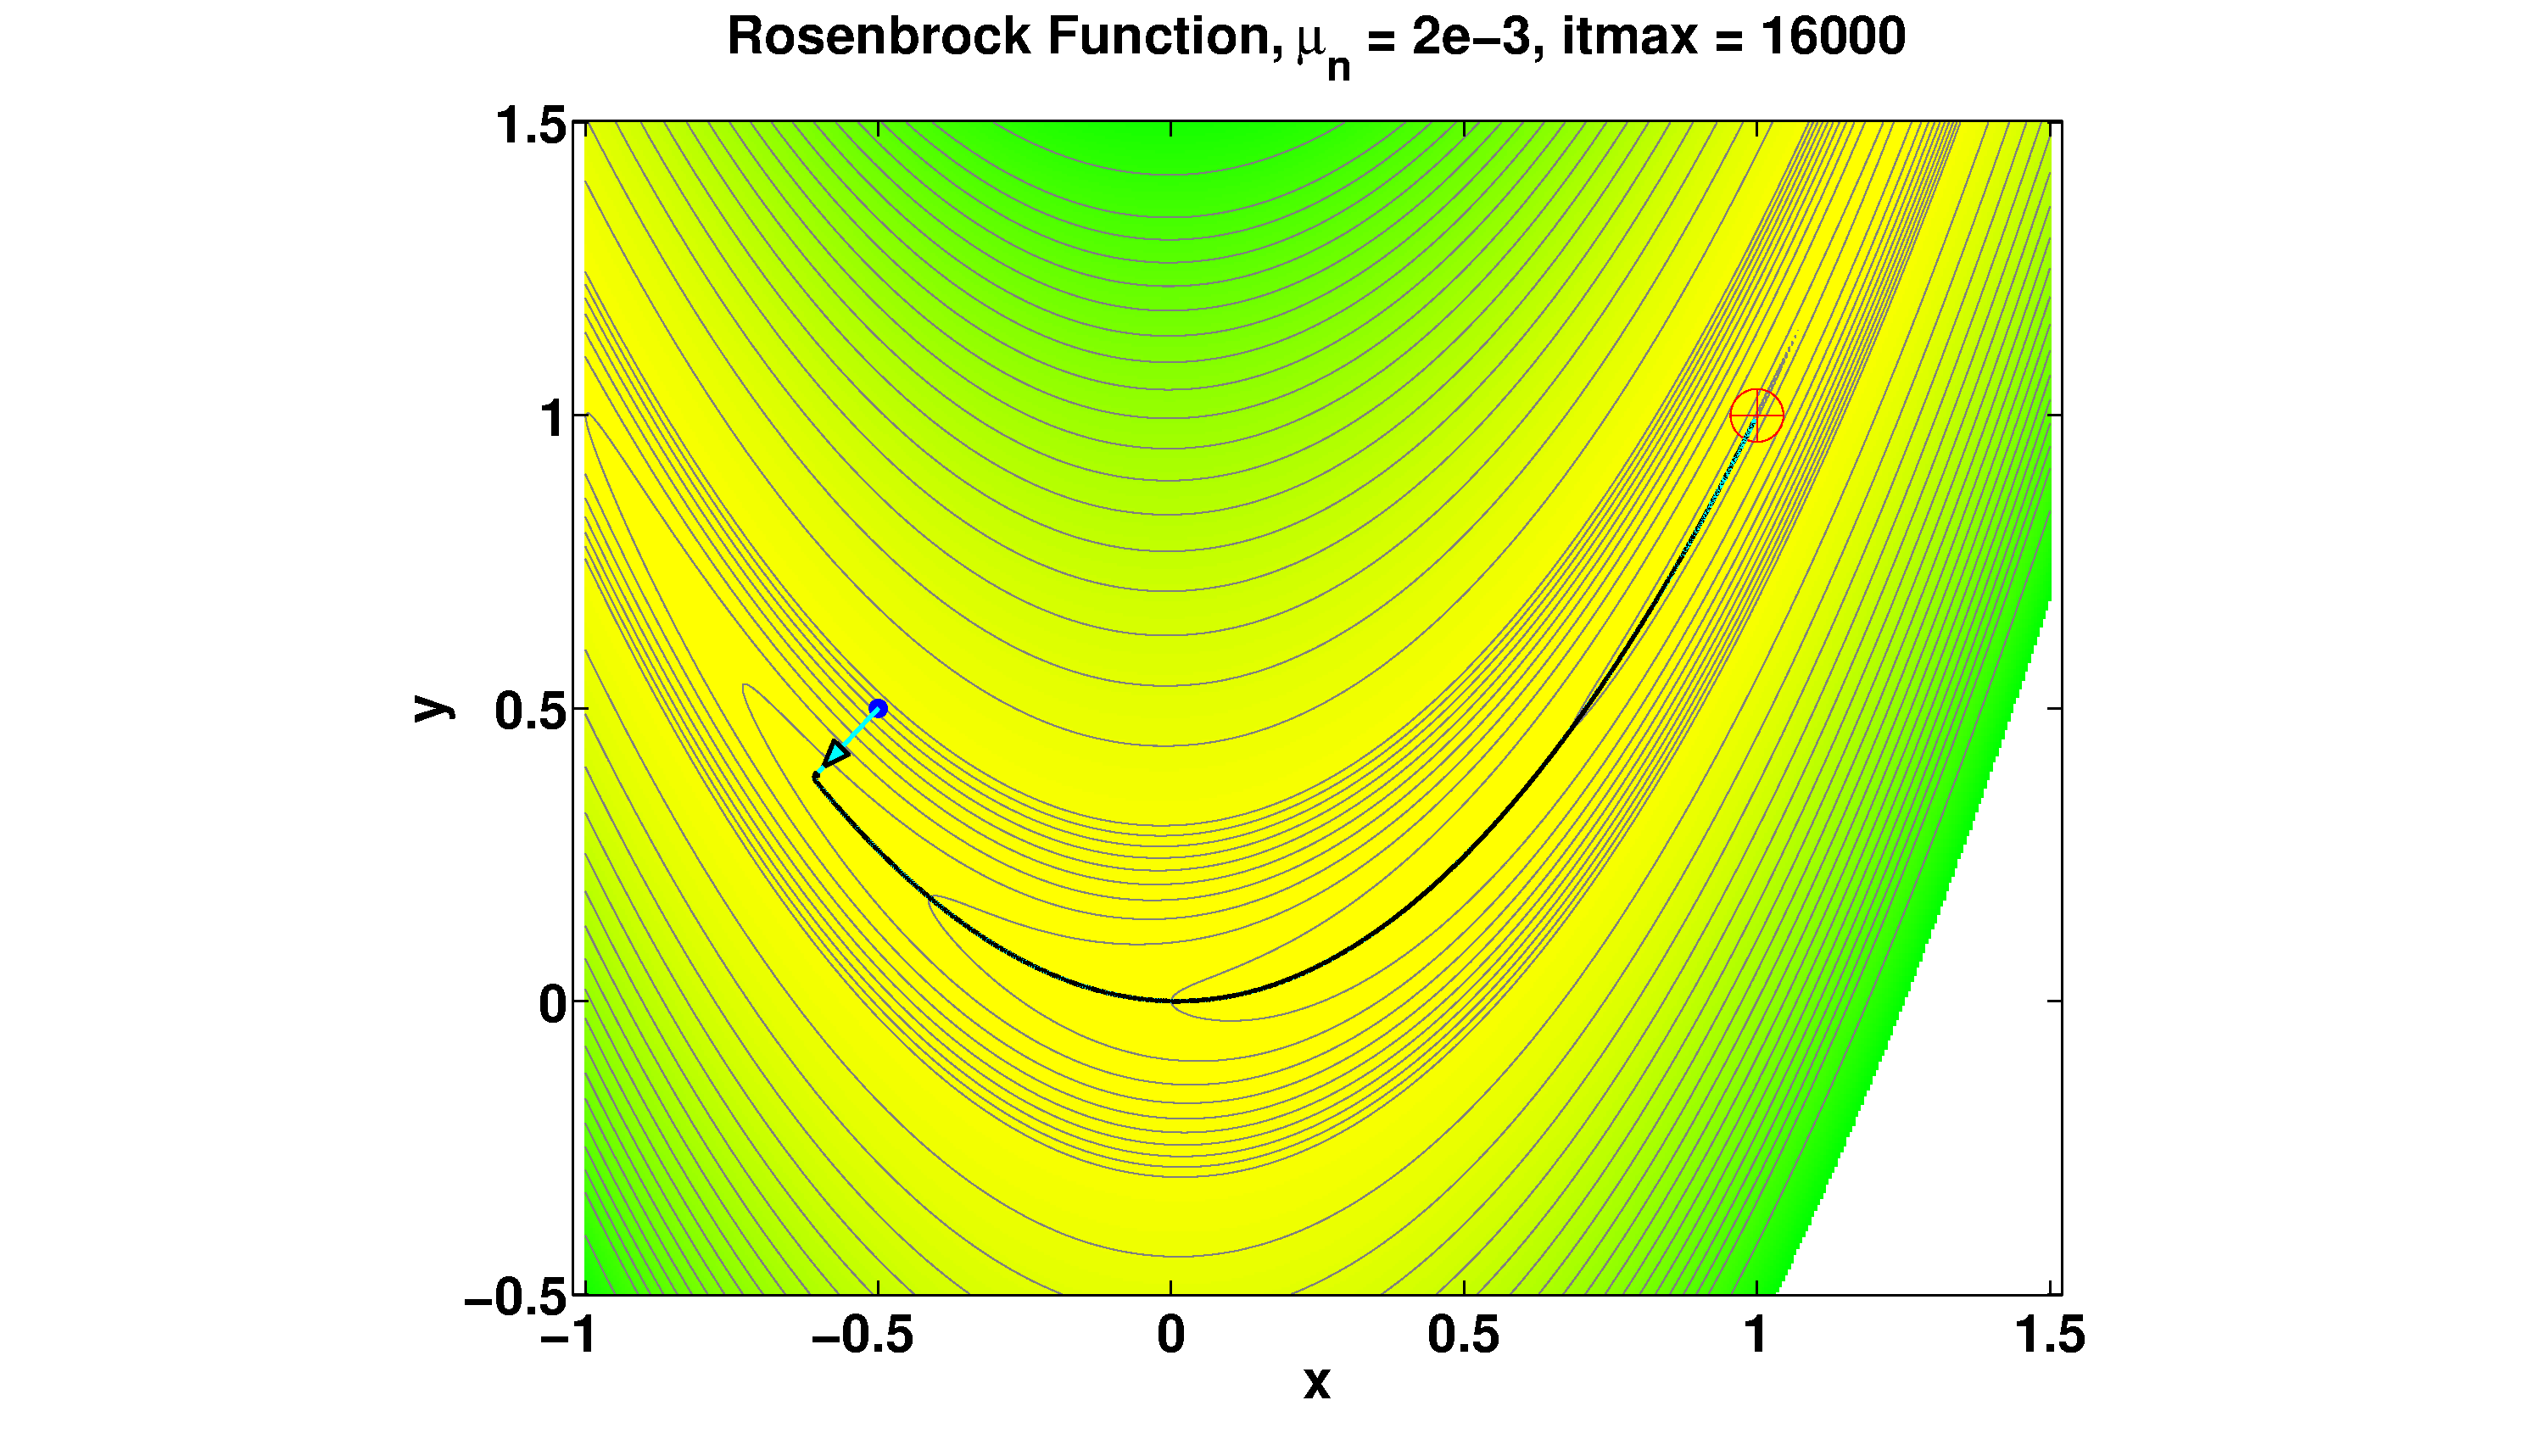
\includegraphics[width=15cm]{figures/Rosenbrock_1.pdf}\\
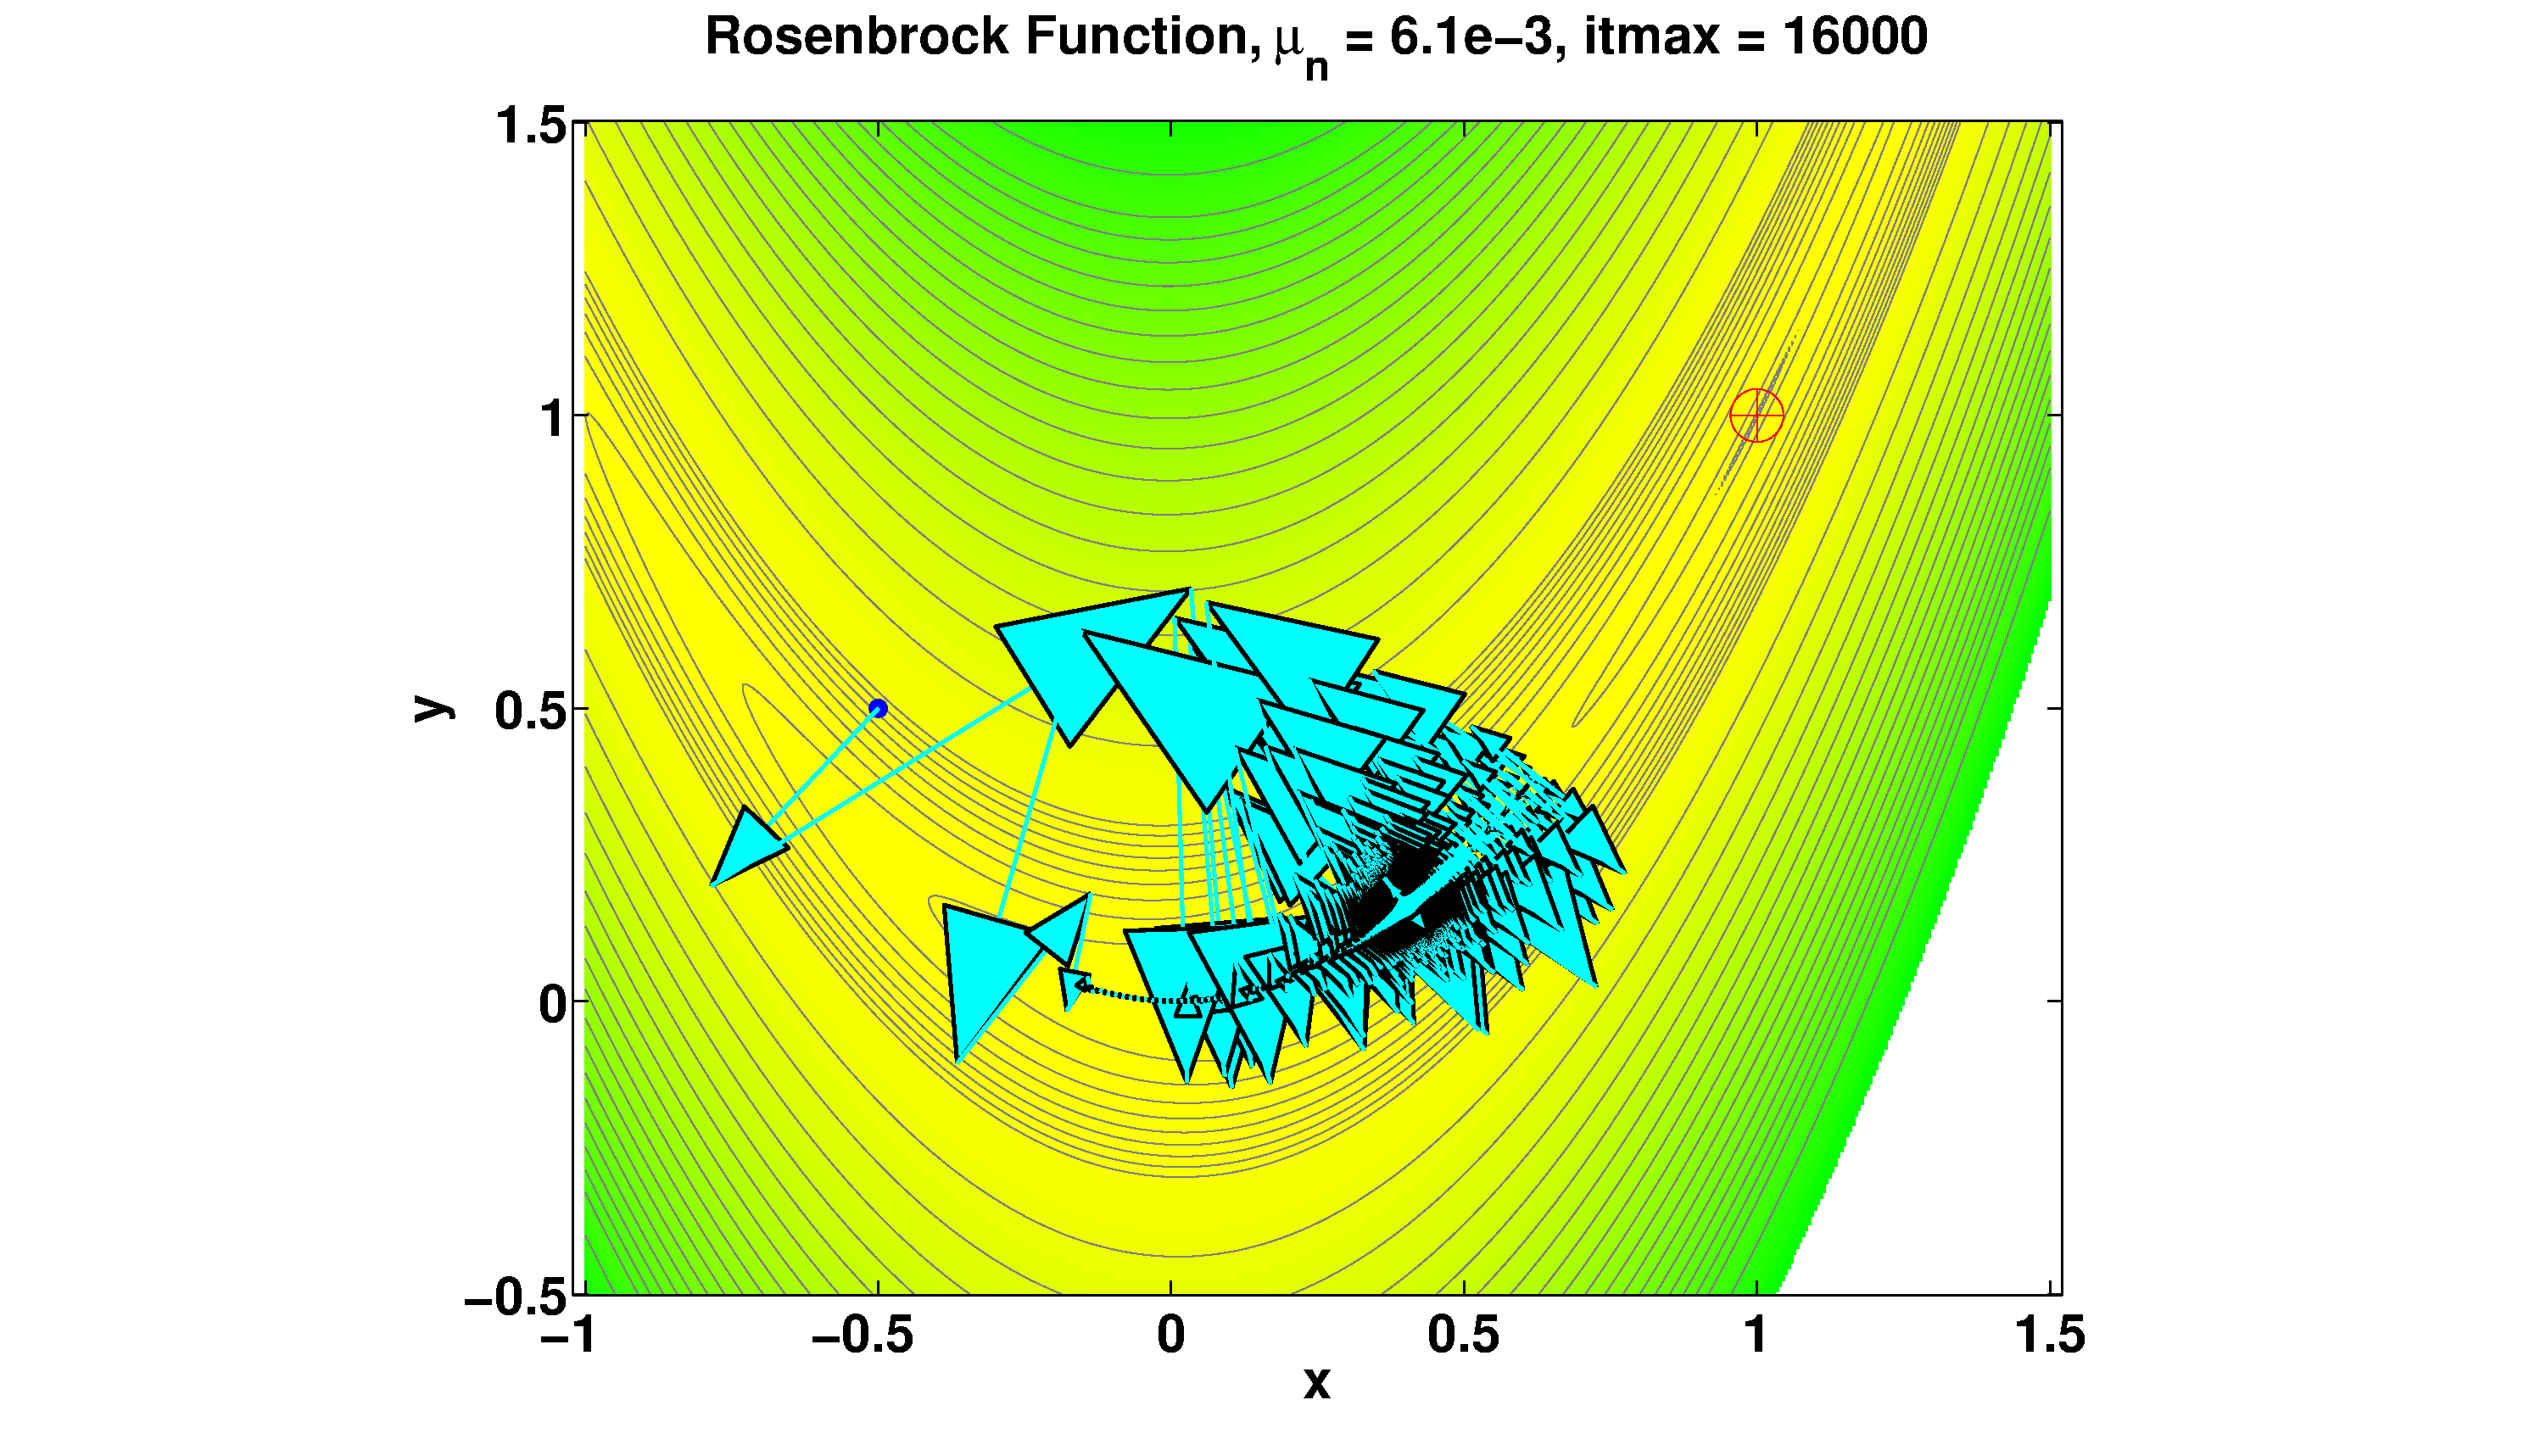
\includegraphics[width=15cm]{figures/Rosenbrock_2.pdf}\\
\caption{Results of the convergence test for the Rosenbrock function. The minimum is marked with a red cross, the starting point with a blue point. The maximum number of iterations is 16000. The step length $\rm{\mu_n}$ varies between $\rm{2e-3}$ (top) and $\rm{6.1e-3}$ (bottom).}
\label{Rosenbrock_constant}
\end{center}
\end{figure}
gradient of the Rosenbrock function is large. After reaching the narrow valley the gradient is much smaller and as a result the model updates are also decreasing. This leads to a very slow convergence speed. Especially near the minimum the model updates become very small. When choosing a larger step length ($\rm{\mu_n=2e-3}$, Fig. \ref{Rosenbrock_constant} (bottom)) the model update is larger even when the gradient is small, but the code fails to converge at all. Instead it is trapped in a narrow part of the valley. To solve this problem a variable step length is introduced.
\begin{figure}[ht]
\begin{center}
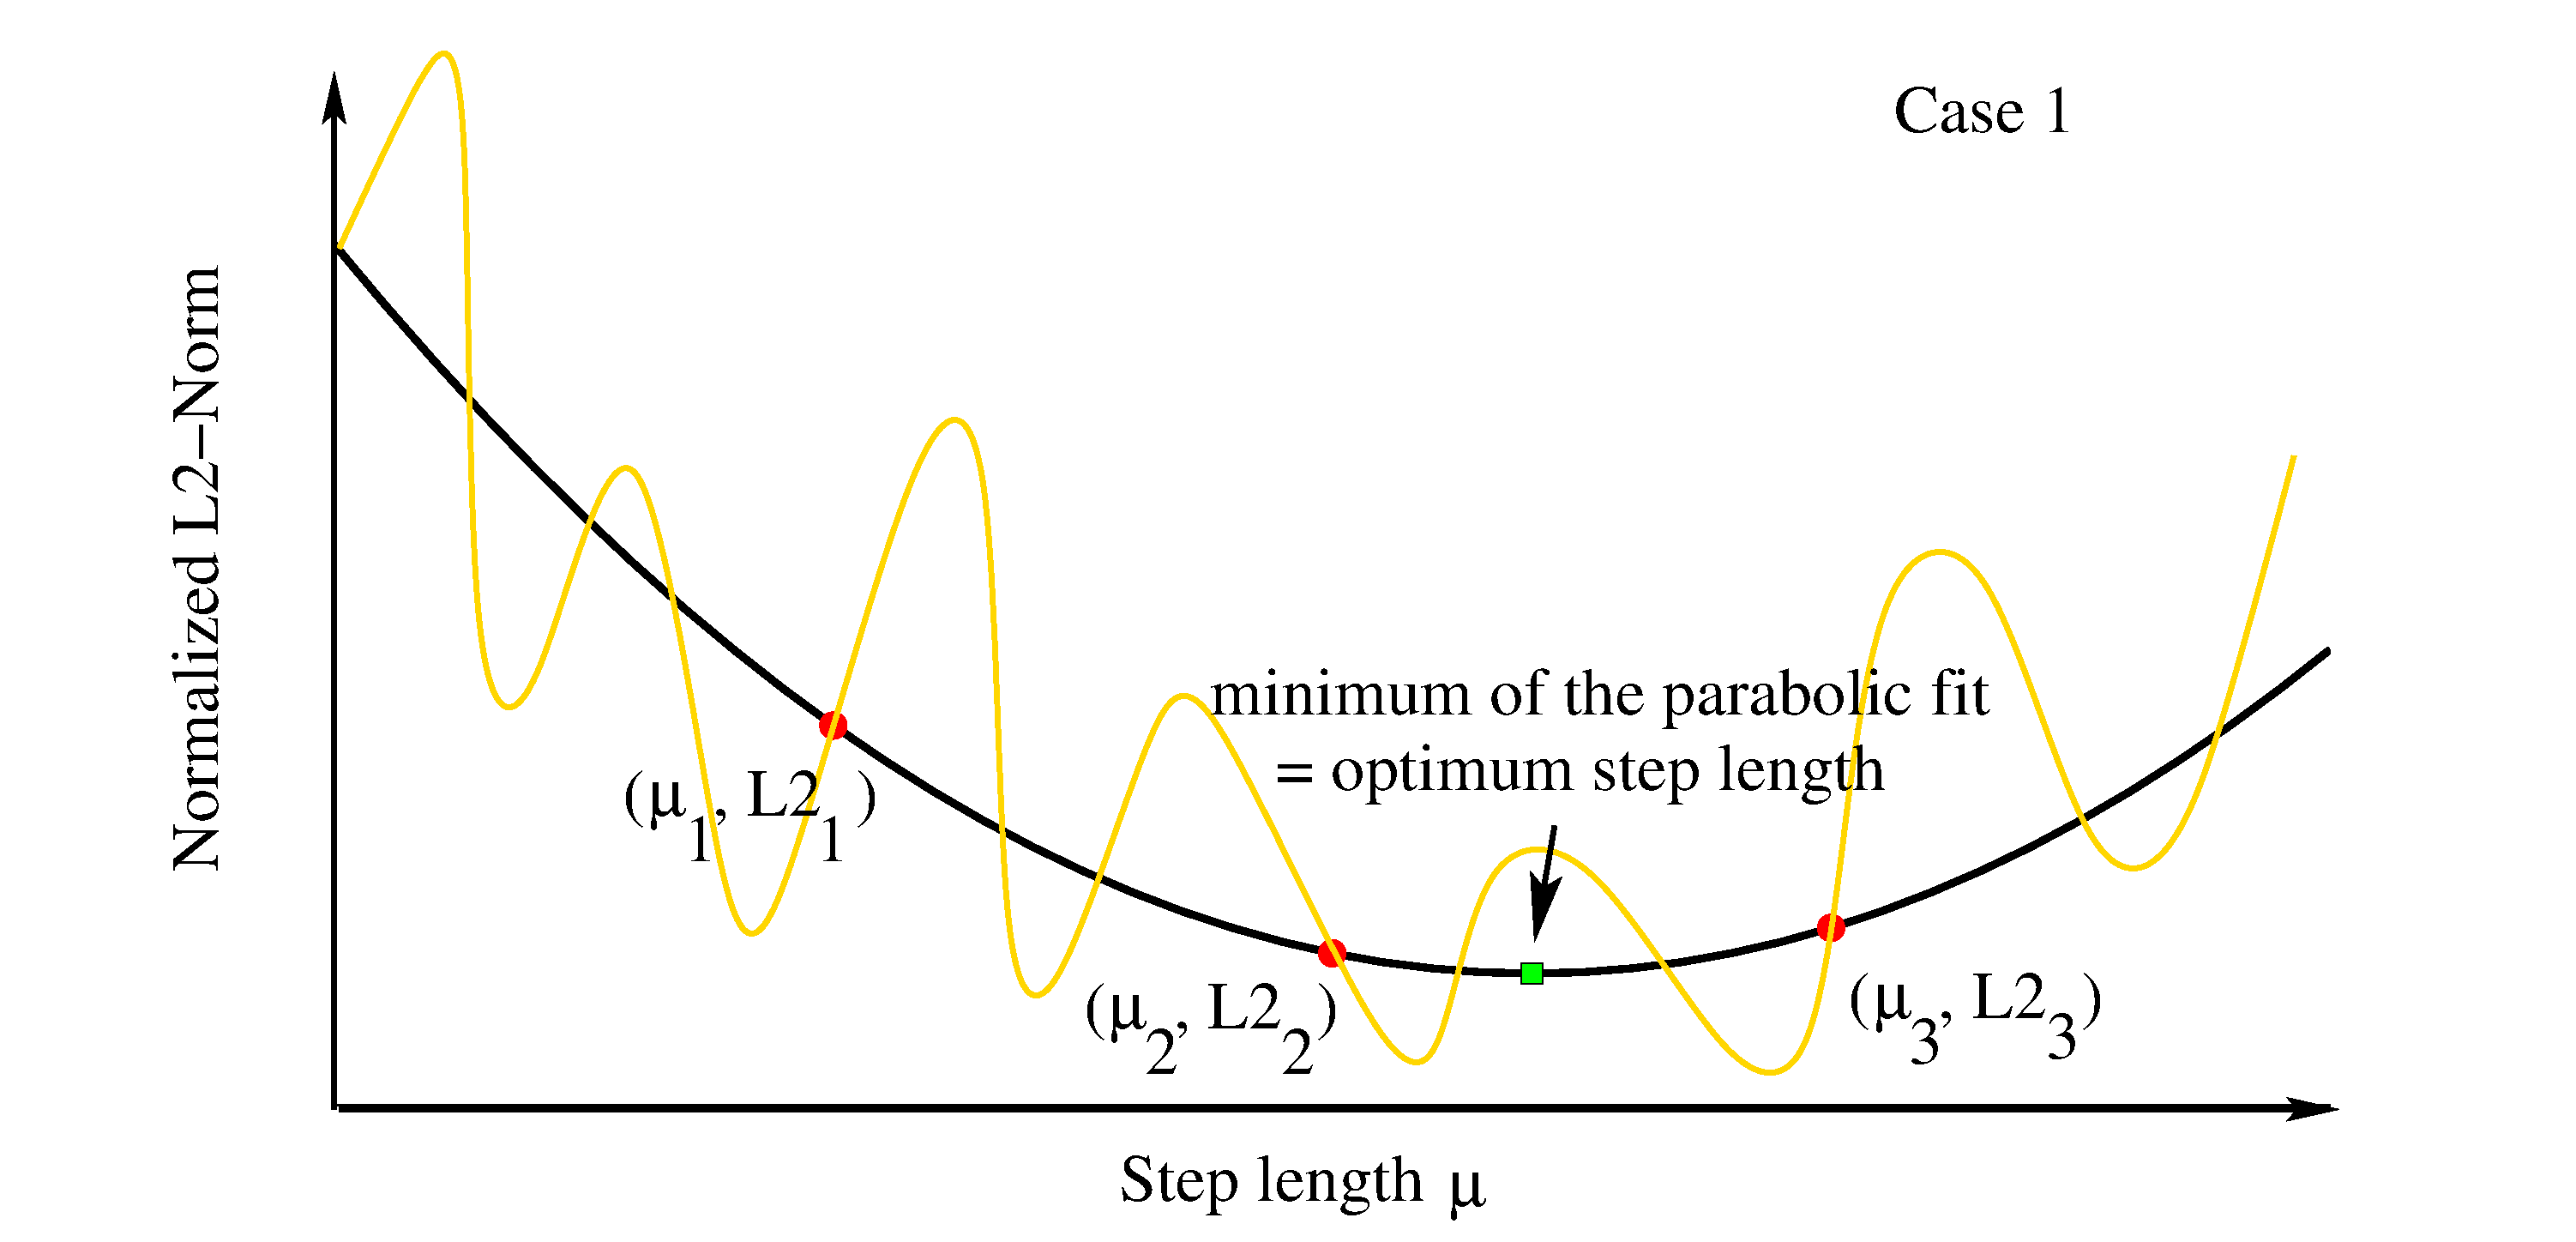
\includegraphics[width=15cm]{figures/sl_case1_final}
\caption{Line search algorithm to find the optimum step length $\rm{\mu_{opt}}$: The true misfit function (yellow line) is approximated by a parabola fitted by 3 points.}
\label{sl_case1_final}
\end{center}
\end{figure}
For three test step lengths $\rm{\mu_1}$, $\rm{\mu_2}$ and $\rm{\mu_3}$ three test models are calculated 
\begin{equation}
\begin{split}
\rm{\mathbf{m_{test1}}} &\rm{= \mathbf{m_{n}} + \mu_1 \delta \mathbf{m'_n}}\\
\rm{\mathbf{m_{test2}}} &\rm{= \mathbf{m_{n}} + \mu_2 \delta \mathbf{m'_n}}\\
\rm{\mathbf{m_{test3}}} &\rm{= \mathbf{m_{n}} + \mu_3 \delta \mathbf{m'_n}}\\
\end{split}
\label{parabola1:1}
\end{equation}              
and the corresponding L2-norms $\rm{L2_1}$, $\rm{L2_2}$ and $\rm{L2_3}$ are estimated (Fig. \ref{sl_case1_final}). The true misfit function (yellow line) can be approximated by fitting a parabola through the three points
\begin{equation}
\rm{L2_i = a \mu_i^2 + b \mu_i + c}
\label{parabola}
\end{equation}              
where $\rm{i \in \{1,2,3\}}$ and a, b, c are the unkown coefficients. 
This system of equations can be written as matrix equation:
\EQ{parabola_fit:1}{
\left(
\begin{array}{lll}
\mu_1^2 & \mu_1 & 1\\
\mu_2^2 & \mu_2 & 1\\
\mu_3^2 & \mu_3 & 1\\
\end{array}
\right)\cdot \hspace{0.2 cm}
\left(
\begin{array}{l}
a \\
b \\
c \\
\end{array}
\right)
=
\left(
\begin{array}{l}
L2_1 \\
L2_2 \\
L2_3 \\
\end{array}
\right) \notag
}
or 
\EQ{parabola_fit:2}{\rm{\mathbf{A}\mathbf{x}=\mathbf{b}}.}
The unknown coefficients of this matrix equation are formally defined by
\EQ{parabola_fit:3}{\rm{\mathbf{x}=\mathbf{A}^{-1}\mathbf{b}},}
In the FWT code the solution vector $\rm{\mathbf{x}}$ is calculated by Gaussian elimination. In the following the step length at the extremum of the parabola is defined the extremum step length $\rm{\mu_{ext}}$ (denoted as green square in Fig.\ref{sl_case1_final}). This extremum step length is   
\EQ{parabola_fit:4}{\rm{\mu_{ext}=-\frac{b}{2a}}.}
The application of the variable step length calculation to the Rosenbrock test problem is shown in Fig. \ref{Rosenbrock_variable}. The number of required iteration steps to reach the minimum is reduced by a factor 4 when compared with the constant step length gradient method. The only problem remaining is the slow convergence speed in the small valley of the Rosenbrock function, due to the fact that the update occurs along the gradient direction of the objective function resulting in a ''criss-cross'' pattern. This behaviour can be avoided by applying a nonlinear conjugate gradient method (chapter \ref{NL_Conjugate_Gradient}). In case of the FWT algorithm the three test step lengths for the individual material parameters are calculated by scaling the maximum of the gradient to the maximum of the actual models:
\begin{equation}
\begin{split}
\rm{\mu_\lambda} &= \rm{p \frac{max(\lambda_n)}{max(\delta \lambda_n)}}\\
\rm{\mu_\mu} &= \rm{p \frac{max(\mu_n)}{max(\delta \mu_n)}}\\
\rm{\mu_\rho} &= \rm{p \frac{max(\rho_n)}{max(\delta \rho_n)}}\\
\end{split}
\end{equation}
For most tests in the following chapters $\rm{p_1=0.0025,\;p_2=0.005,\;p_3=0.01}$, which corresponds to maximum model changes of 1/4, 1/2 and 1 \%, worked very well for the optimum step length estimation. All material parameters are updated at the same time. To save computational time the corresponding $\rm{L_2}-$norms are calculated for a few representative shots (in most cases 3). For the acoustic case the step length estimation by parabolic fitting works very well and leads to a smooth decrease of the misfit function during the FWT (Kurzmann (2007), personal communication, \cite{kurzmann:08}). For the multiparameter elastic FWT the misfit function consists of more local minima and therefore the decrease of the objective function is not as smooth as in the acoustic case. \cite{brossier:2009} proposed a more intensive bracketing stage before applying the parabolic fit. For $\rm{p_1=0.0}$ the test step lengths $\rm{p_2}$ and $\rm{p_3}$ are calculated to satisfy the following criteria:
\begin{equation}
\begin{split}
&\rm{L2_2(\mathbf{m_{test2}} = \mathbf{m_{n}} + \mu_2 \delta \mathbf{m'_n}) < L2_1(\mathbf{m_{test1}} = \mathbf{m_{n}})}\\
&\rm{L2_3(\mathbf{m_{test3}} = \mathbf{m_{n}} + \mu_3 \delta \mathbf{m'_n}) > L2_2(\mathbf{m_{test2}} = \mathbf{m_{n}} + \mu_2 \delta \mathbf{m'_n})}\\
\end{split}
\label{parabola1:1:100}
\end{equation}              
This approach leads to a smoother decrease of the objective function, but also increases the number of required forward models.         
\begin{figure}[ht]
\begin{center}
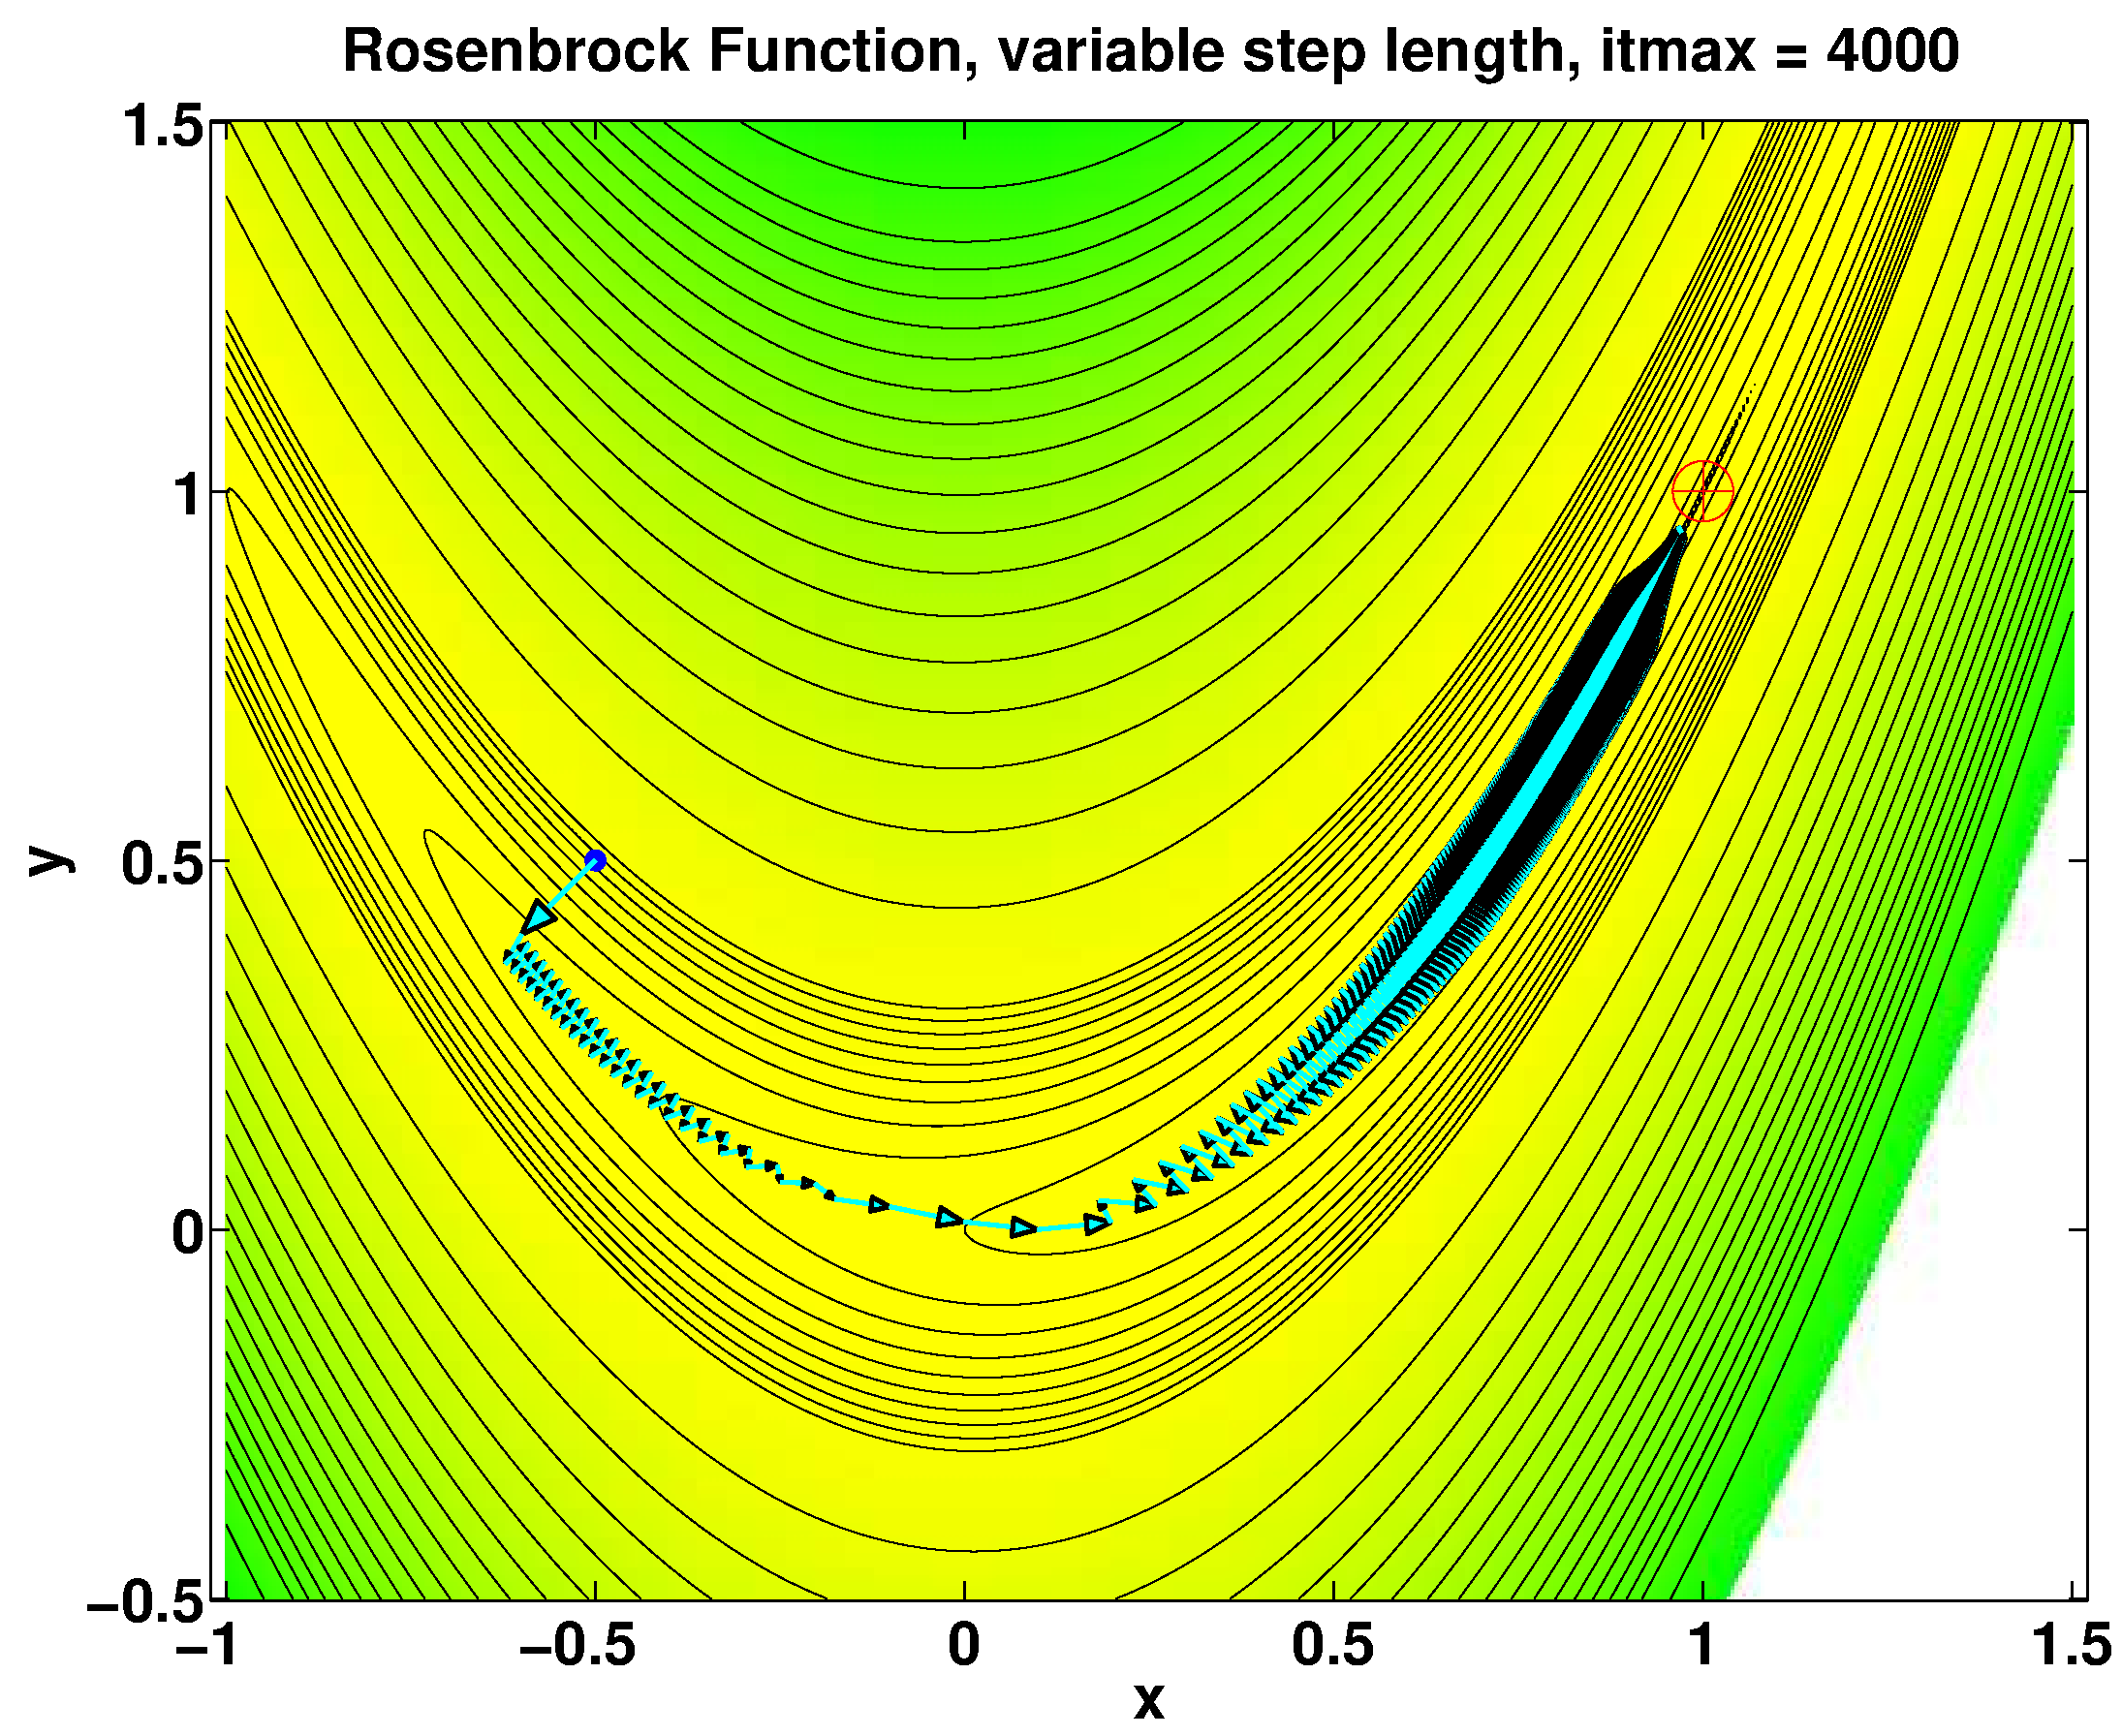
\includegraphics[width=16cm]{figures/Rosenbrock_3}
\caption{Results of the convergence test for the Rosenbrock function. The minimum is marked by a red cross, the starting point by a blue point. The maximum number of iterations is 4000. The optimum step length is calculated at each iteration by the parabola fitting algorithm. Note the criss-cross pattern of the updates in the narrow valley near the minimum.}
\label{Rosenbrock_variable}
\end{center}
\end{figure}
\section{Nonlinear Conjugate Gradient Method}\label{NL_Conjugate_Gradient} 
To increase the convergence speed in narrow valleys it would be better to update the model at iteration step n not exactly along the gradient direction $\rm{\delta \mathbf{m}_n}$, but along the conjugate direction $\rm{\delta \mathbf{c}_n}$
\begin{equation}
\rm{\delta \mathbf{c}_n = \delta \mathbf{m}_n + \beta_n \delta \mathbf{c}_{n-1},}  
\label{conj1}
\end{equation}
The first iteration step (n=1) consists of a model update along the steepest descent direction:
\begin{equation} 
\rm{\mathbf{m}_{2} = \mathbf{m}_{1} + \mu_1 \mathbf{\delta m}_{1}, }
\label{conj1:1}
\end{equation}
For all subsequent iteration steps ($\rm{n>1}$) the model is updated along the conjugate direction:
\begin{equation} 
\rm{\mathbf{m}_{n+1} = \mathbf{m}_{n} + \mu_n \mathbf{\delta c}_{n}, }
\label{conj1:2}
\end{equation}
where $ \rm{\delta \mathbf{c}_{1} = \delta \mathbf{m}_1}$.
The weighting factor $\rm{\beta}$ can be calculated in different ways:
\begin{enumerate}
\item Fletcher-Reeves:\\
\begin{equation}
\rm{\beta^{FR}_n=\frac{\delta \mathbf{m}^T_n \delta \mathbf{m}_n}{\delta \mathbf{m}^T_{n-1} \delta \mathbf{m}_{n-1}}}
\label{conj2}
\end{equation}
\item Polak-Ribi$\rm{\acute{e}}$re:\\
\begin{equation}
\rm{\beta^{PR}_n=\frac{\delta \mathbf{m}^T_n (\delta \mathbf{m}_n - \delta \mathbf{m}_{n-1})}{\delta \mathbf{m}^T_{n-1} \delta \mathbf{m}_{n-1}}}
\label{conj3}
\end{equation}
\item Hestenes-Stiefel:\\
\begin{equation}
\rm{\beta^{HS}_n=\frac{\delta \mathbf{m}^T_n (\delta \mathbf{m}_n - \delta \mathbf{m}_{n-1})}{\delta \mathbf{c}^T_{n-1} (\delta \mathbf{m}_n - \delta \mathbf{m}_{n-1})}}
\end{equation}
\end{enumerate}
I use the very popular choice $\rm{\beta_n = max[0,\beta_n^{PR}]}$ which provides an automatic direction reset. This is important because subsequent search directions lose conjugacy requiring the search direction to be reset to the steepest descent direction. Note that the conjugate gradient method doesn't require any additional computational time because only the gradient $\rm{\delta \mathbf{m}_n}$ at two subsequent iterations has to be known. The application of the nonlinear conjugate gradient method combined with the variable step length calculation to the Rosenbrock function is shown in Fig. \ref{Rosenbrock_cg}. The criss-cross pattern of the steepest descent method has vanished. The conjugate gradient method converges already after 2000 iterations compared with 4000 iteration steps of the pure gradient method.   

\begin{figure}[ht]
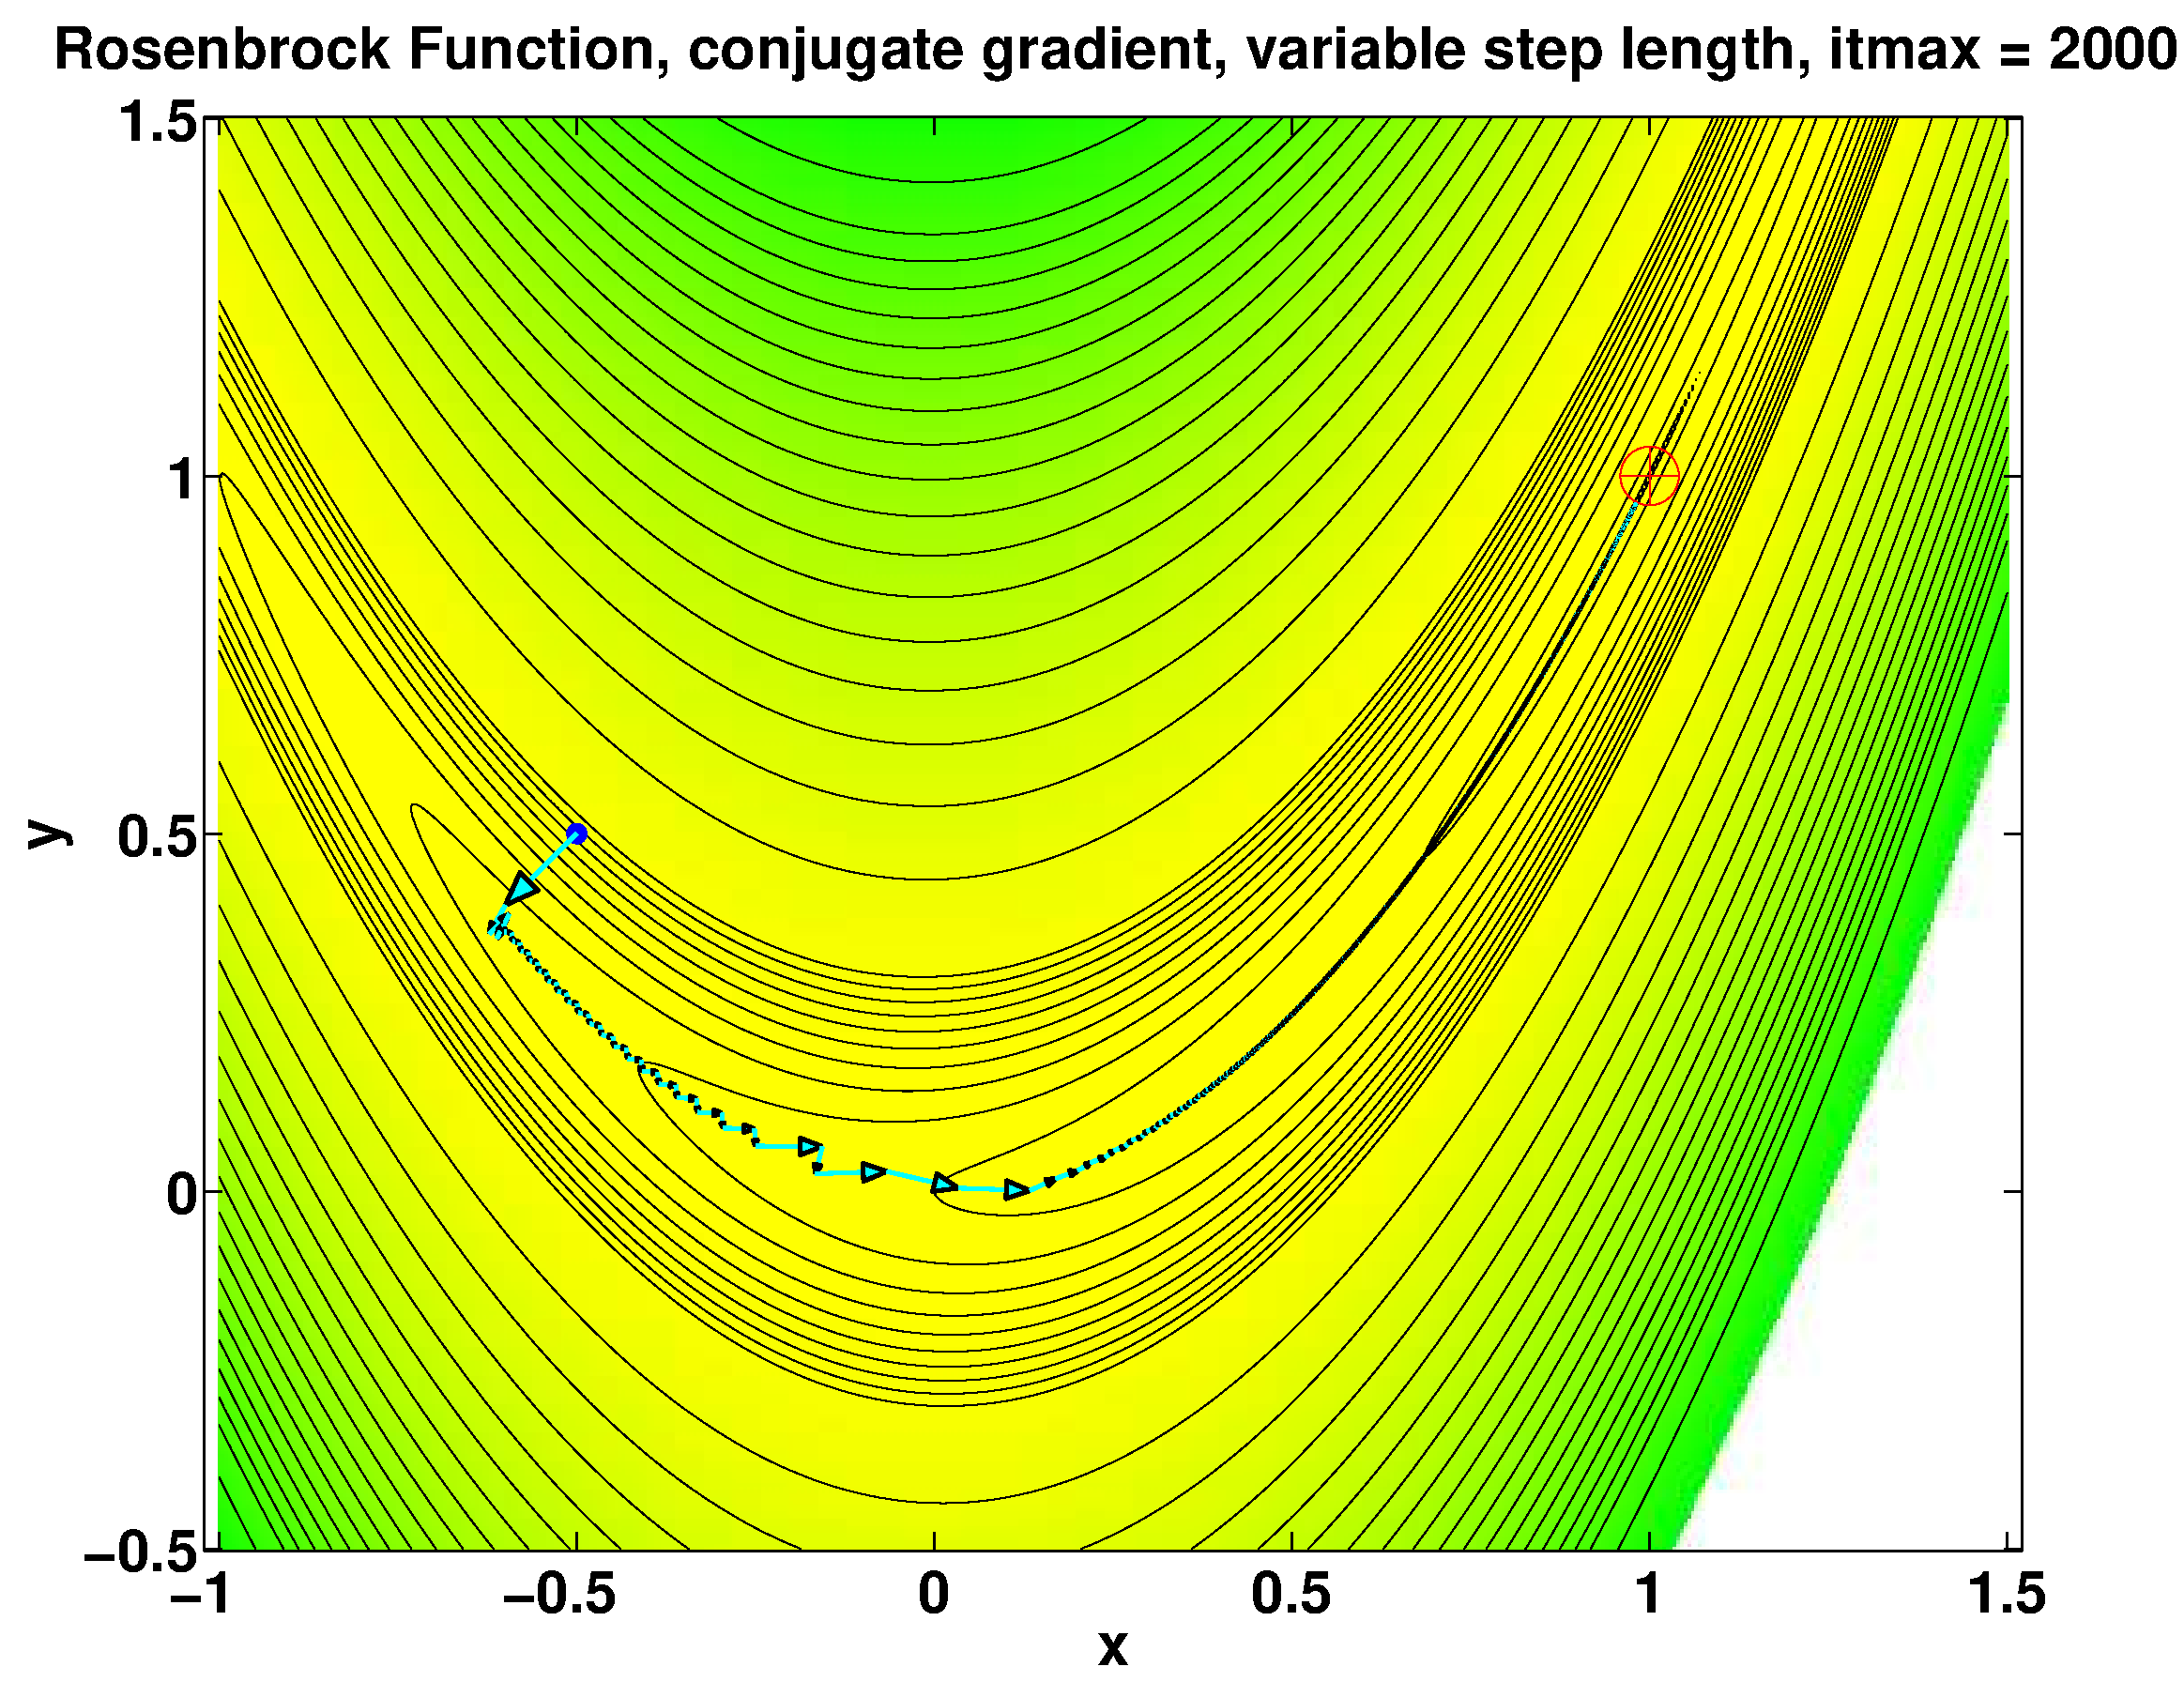
\includegraphics[width=17cm]{figures/Rosenbrock_4}\\
\caption{Results of the convergence test for the Rosenbrock function using the conjugate gradient method, where the optimum step length is calculated with the parabolic fitting algorithm. The minimum is marked by a red cross, the starting point by a blue point. The maximum number of iterations is 2000.}
\label{Rosenbrock_cg}
\end{figure}

\clearpage
\section{The elastic FWT algorithm}
In summary the FWT algorithm consists of the following steps:

\begin{enumerate}
\item Define a starting model $\rm{\mathbf{m_1}}$ in the parameter space. This model should represent the long wavelength part of the underground 
very well, because the FWT code is only capable to reconstruct structures at or below the dominant seismic wavelength due to its slow 
convergence speed, the nonlinearity of the problem and the inherent use of the Born approximation to calculate the gradient direction.
\item At iteration step n do:
\begin{enumerate} 
\item For each shot solve the forward problem, stated in Eq.(\ref{2:1}) for the actual model $\rm{\mathbf{m}_n}$ to generate a synthetic dataset 
      $\rm{\mathbf{u^{mod}}}$ and the wavefield $\rm{\mathbf{u}(\mathbf{x},t)}$. 
\item Calculate the residual seismograms $\rm{\delta \mathbf{u} = \mathbf{u^{mod}} - \mathbf{u^{obs}}}$ for the x- and y-components of the
seismic data.
\item Generate the wavefield $\rm{\mathbf{\Psi}(\mathbf{x},t)}$ by backpropagating the residuals from the receiver postions.
\item Calculate the gradients $\rm{\delta \mathbf{m}_n}$ of each material parameter according to Eqs.(\ref{2:28}).
\item To increase the convergence speed an appropriate preconditioning operator P is applied to the gradient $\rm{\delta \mathbf{m}}$
\begin{equation}
\rm{\delta \mathbf{m}^p_n = P \delta \mathbf{m}_n}
\label{2:26:1} 
\end{equation}
Examples of simple preconditioning operator are given in chapter \ref{marmousi_complex_FWT} for a reflection geometry. 
\item For a further increase of the convergence speed calculate the conjugate gradient direction for iteration steps $\rm{n \ge 2}$: 
\begin{equation}
\rm{\delta \mathbf{c}_n = \delta \mathbf{m}^p_n + \beta \delta \mathbf{c}_{n-1}},\; \rm{\text{with}}\; \rm{\delta \mathbf{c}_{1} = \delta
\mathbf{m}^p_1}  
\label{2:26:2}
\end{equation}
where the weighting factor 
\begin{equation}
\rm{\beta^{PR}=\delta \mathbf{m}^p_n \frac{\delta \mathbf{m}^p_n - \delta \mathbf{m}^p_{n-1}}{\delta \mathbf{m}^p_{n-1} \delta \mathbf{m}^p_{n-1}}}
\label{FWT_alg:1}
\end{equation} 
by Polak-Ribi$\rm{\acute{e}}$re is used. The convergence of the Polak-Ribi$\rm{\acute{e}}$re method is guaranteed by choosing 
$\rm{\beta=max[\beta^{PR},0]}$.  
\item Estimate the step length $\rm{\mu_n}$ by the line search algorithm described in chapter \ref{optimum_step_length}.
\item Update the material parameters using the gradient method 
\begin{equation}
\rm{\mathbf{m}_{n+1} = \mathbf{m}_{n} - \mu_n \delta \mathbf{c}_n.}
\end{equation}
If the material parameters are not coupled by empirical relationships it is important to update all three elastic material parameters 
at the same time, otherwise strong artefacts may dominate the inversion result, especially in the case of very complex media.  
\end{enumerate}
\item If the residual energy E is smaller than a given value stop the iteration. Otherwise continue with the next iteration step.  
\end{enumerate}

%------------------------------------------------------------------------------------------------%
\chapter{\label{cha:STF-Inversion}Source Time Function Inversion}
\textbf{Introduction:}\\
To remove the contribution of the unknown source time function (STF) from the waveform residuals, it is necessary to design a filter which minimizes the misfit to the field recordings and raw synthetics. The library libstfinv from Thomas Forbriger was exported from TFSoftware and can be used with a C API in DENISE. The purpose of this library is to provide methods for the derivation of source-time-functions in approaches to full waveform inversion. Given a set of recorded data and a set of synthetic data (typically, but not necessarilly the impulse response of the subsurface) a source time function is obtained due to some optimization citerion. The synthetic waveforms are convolved with this wavelet and the convolved synthetics as well as the wavelet itself are returned to the user.

The source time wavelet in this context not necessarily is the actual force time history of the source used in the experiment or a similar quantity of physical meaning. The source time wavelet simply is the wavelet which minimizes the misfit between synthetic and recorded waveforms due to some misfit condition, if the synthetics are concolved with this wavelet. In particular this implies that the synthetics not necessarily must be the impulse response (Greens function) of the subsurface, they may simply be synthetic waveform computed for some generic source wavelet (like a Ricker wavelet). The derived source time function then have to be understood with respect to this generic wavelet.\\
\newline
The library provides different engines to find an optimal source time wavelet. The basic steps of operation are:
\begin{enumerate}
 \item An engine is initialized. At this step pointers to arrays are passed to the engine together with some header information. The engines memorizes these pointers and expects to find the recorded data as well as the synthetics at the inidcated locations in memory.
 \item The run()-function of the engine is called. The engine takes the recorded and synthetic data currently found at the memory arrays, calculates an optimzed wavelet and returns the wavelet together with the convolved synthetics by copying them to the memory locations inidicated by the initializer of the engine. This step is repeated after each computation of synthetic data.
 \item The engine is removed once the iteration of inversion is terminated.
\end{enumerate}
\textbf{How to construct parameter strings:}\\
A specific engine is selected by passing a parameter string to the library interface. This parameter string may further contain parameters to control the execution mode of the engine. The parameter string starts with an ID-sequence identifying the desired engine. In the parameter string the ID-sequence is terminated by a colon (:).\\

After selecting the desired engine, the interface function strips of the ID-sequence as well as the colon from the parameter string and initializes the engine, passing the references to user workspace as well as the rest of the parameter string. The rest of the parameter string may consist of several control parameters being separated by colons (:). Each control parameter may just be a flag (switch to turn an option on) or may come along with a parameter value. The value of the parameter is separated by an equal sign (=).

Examples:
\begin{itemize}

        \item To select frequency domain least squares and shift the returned source time function by 0.4s and switch on verbose mode, pass the following parameter string:\\
        \textit{fdlsq:tshift=0.4:verbose} 


        \item To select frequency domain least squares, apply offset dependent weights and use a power of two to speed up the FFT:\\
        \textit{fdlsq:pow2:exp=1.4} 
\end{itemize}
\textbf{Detailed description of the engine 'Fourier domain least squares (fdlsq)'}\\
If
\begin{itemize}
     \item $d_{lk}$ is the Fourier coefficient of recorded data at Frequency
       $f_l$ and receiver $k$ at offset $r_k$,
     \item $s_{lk}$ is the Fourier coefficient of the corresponding
       synthetics and
     \item $q_l$ is that of the sought source time function,
\end{itemize}
then this engine will minimize the objective function\\
     \begin{equation}
       E=\sum\limits_{l,k}\left|w_{lk}\,
          \left(d_{lk}-s_{lk}q_l\right)
       \right|^2+\sum\limits_{l}\lambda^2\left|q_l\right|^2
       =\chi^2+\psi^2
     \end{equation}
     with respect to the real part $q_l^\prime$ and the
     imaginary part $q_l^{\prime\prime}$ of 
     \begin{equation}
       q_l=q_l^\prime+i\,q_l^{\prime\prime}.
     \end{equation}
     In the above expression
     \begin{equation}
       \chi^2=\sum\limits_{l,k}\left|w_{lk}\,
               \left(d_{lk}-s_{lk}q_l\right)
                \right|^2
     \end{equation}
     is the data misfit with weights $w_{lk}$ and
     \begin{equation}
       \psi^2=\sum\limits_{l}\lambda^2\left|q_l\right|^2
     \end{equation}
     is used for regularization and will introduce a water-level in the
     deconvolution.
     $\lambda$ will balance both contributions.
     The conditions
     \begin{equation}
       \frac{\partial E}{\partial q_l^\prime}\stackrel{!}{=}0
       \quad\wedge\quad
       \frac{\partial E}{\partial q_l^{\prime\prime}}\stackrel{!}{=}0
     \end{equation}
     result in (\cite{Forbriger:01}, appendix A.3)
     \begin{equation}
       q_l=\frac{
         \eta^2\sum\limits_{k}f_k^2\,s_{kl}^\ast\,d_{kl}
       }{
         \lambda^2+\eta^2\sum\limits_{k}f_k^2\,s_{kl}^\ast\,s_{kl}
       }
       \quad\forall\, l
     \end{equation}
     where
     \begin{equation}
       w_{lk}=\eta\,f_k
     \end{equation}
     and $f_k$ is a receiver specific weighting factor.
     Now $\eta$ and $\lambda$ have to be used to balance the
     regularization.
     We aim to specify a waterlevel as a fraction of synthetic data energy.\\
\newline
      
     \textbf{Setting up the waterlevel:}\\
     The misfit equals one if the scaled energy of the residual
     $d_{lk}-s_{lk}q_l$ equals the scaled energy of the synthetics
     $s_{lk}$ and
     \begin{equation}
       \eta^2=\frac{1}{\sum\limits_k f_k^2\sum\limits_l \left|s_{lk}\right|^2}
     \end{equation}
     is the reciprocal of the scaled energy of the synthetics.
     If we then choose
     \begin{equation}
       \frac{\lambda^2}{\eta^2}=\frac{\epsilon^2}{N\eta^2}=
         \frac{\epsilon^2}{N}\sum\limits_k f_k^2\sum\limits_{l=0}^{N-1}
        \left|s_{lk}\right|^2
     \end{equation}
     where $N$ is the number of frequencies, then $\epsilon^2$
     will specify a waterlevel as a fraction of the scaled energy of the
     synthetics.\\
\newline
    
     \textbf{Using Parceval's Theorem to calculate signal energy:}\\
     Parceval's Theorem for a signal $a(t)$ and its Fourier transform 
     $\tilde{a}(\omega)$ is
     \begin{equation}
       \int\limits_{-\infty}^{+\infty}\bigl|a(t)\bigr|^2\,\textrm{d} t=
       \int\limits_{-\infty}^{+\infty}\bigl|\tilde{a}(\omega)\bigr|^2\,
         \frac{\textrm{d} \omega}{2\pi}.
     \end{equation}
     If $S_{jk}$ are the time series samples corresponding to the Fourier
     coefficients $\tilde{s}_{lk}$ and $\Delta t$ is the sampling
     interval then
     \begin{equation}
       \sum\limits_{k=0}^{M-1}\left|S_{jk}\right|^2\,\Delta t=
       \sum\limits_{l=0}^{M-1}\left|\tilde{s}_{lk}\right|^2\,\frac{1}{M\,\Delta t},
     \end{equation}
     where $M=2N$ is the number of samples in the time series.
     In the above calculation the energy sum only uses the positive
     frequencies and
     \begin{equation}
       \sum\limits_k f_k^2\sum\limits_{l=0}^{N-1}\left|\tilde{s}_{lk}\right|^2
       =
         N\,(\Delta t)^2\,
         \sum\limits_k f_k^2
         \sum\limits_{j=0}^{2N-1}\left|S_{jk}\right|^2.
     \end{equation}
     Fourier coefficients $s_{lk}$ calculated by the
     stfinv::STFFourierDomainEngine are not scaled (see documentation of
     libfourierxx and libfftw3), such that
     \begin{equation}
       \Delta t\,s_{lk}=\tilde{s}_{lk}
     \end{equation}
     (both, $s_{lk}$ and $\tilde{s}_{lk}$ are Fourier coefficients).
     Consequently
     \begin{equation}
       \sum\limits_k f_k^2\sum\limits_{l=0}^{N-1}\left|s_{lk}\right|^2
       =
         N\,
         \sum\limits_k f_k^2
         \sum\limits_{j=0}^{2N-1}\left|S_{jk}\right|^2.
     \end{equation}
    
     \textbf{Final calculation recipe:}\\
     The solution to our problem is
     \begin{equation}
       q_l=\frac{
         \sum\limits_{k}f_k^2\,s_{lk}^\ast\,d_{lk}
       }{
         \epsilon^2\,\sum\limits_k f_k^2
                    \sum\limits_{j=0}^{2N-1}\left|S_{jk}\right|^2
               +\sum\limits_{k}f_k^2\,s_{lk}^\ast\,s_{lk}
       }
       \quad\forall\, l,
     \end{equation}
     where
     \begin{equation}
       \sum\limits_{j=0}^{2N-1}\left|S_{jk}\right|^2
     \end{equation}
     is the sum of the squared sample values $S_{jk}$ of the synthetic
     time series for receiver $k$, $f_k$ are the scaling factors, and $\epsilon^2$
     is the water level parameter.
\newline
     
Author: Thomas Forbriger.
\newline

For more information see \href{http://www.opentoast.de/Data_analysis_code_soutifu_and_libstfinv.php}{http://www.opentoast.de/Data\_analysis\_code\_soutifu\_and\_libstfinv.php} .

%------------------------------------------------------------------------------------------------%

\chapter{\label{cha:Getting-Started}Getting Started}

%------------------------------------------------------------------------------------------------%

In the following sections, we give a short description of the different modeling  parameters, options and how the program is used in a parallel MPI environment.

\section{Requirements}
The parallelization employs functions of the Message Passing Interface (MPI). MPI has to be installed when compiling and running the DENISE software. At least two implementations exist for Unix-based networks: OpenMPI and MPICH2. The LAM-MPI implementation is no longer supported by the developers. Currently all three implementation work with DENISE. OpenMPI and MPICH2 are MPI programming environments and development systems for heterogeneous computers on a network. With OpenMPI or MPICH2, a dedicated cluster or an existing network computing  infrastructure can act as one parallel computer solving one problem. The latest version of OpenMPI can be obtained from \href{http://www.open-mpi.org}{http://www.open-mpi.org}.% MPICH2 is available at \href{http://www.open-mpi.org}{http://www-unix.mcs.anl.gov/mpi/mpich}. LAM-MPI can be downloaded here: \href{http://www.lam-mpi.org}{http://www.lam-mpi.org}.


\section{Installation}
\label{installation}
After unpacking the software package (e.g. by \textit{tar -zxvf DENISE.tgz}) and changing to the directory DENISE (\textit{cd DENISE})  you will find different subdirectories:

\textbf{bin}\\
This directory contains all executable programs, generally DENISE and snapmerge. These executables are generated using the command \textit{make $<$program$>$} (see below).

\textbf{contrib}\\
This directory contains external contributions to DENISE.

\textbf{doc}\\
This directory contains documentation on the software (this users guide) as well as some important papers in PDF format on which the software is based on (see above).

\textbf{genmod}\\
Contains the model and benchmark files for DENISE.

\textbf{mfiles}\\
Here some Matlab routines (m-files) are stored. These Matlab programs can be used to find optimal relaxation frequencies to approximate a constant Q (qapprox.m) or to plot Q as a function of frequency for certain relaxation frequencies and value of tau (qplot.m). It is necessary to have the Matlab Optimization Toolbox installed. For further details we refer to \cite{bohlen:98} and to the paper in which the so-called tau-method is described \cite{blanch:95}.

\textbf{par}\\
Parameter files for DENISE modeling.

% \textbf{scripts}\\
% Here, you will find examples of script-files used to submit modeling jobs on cluster-computers.

\textbf{src}\\
This directory contains the complete source codes.  The following programs are available and may be compiled using make $<$program$>$.


\section{Compilation of DENISE}\label{compexec}
Before compiling the main program DENISE you have to compile the required additional libraries e.g. for timedomain filtering, the inversion for the correction filter for the unknown source time function and so on. In the DENISE/par directory simply use:
\newline

\textit{make}
\newline

which will install the following libraries:

{\color{blue}{\begin{verbatim}
lib cseife
lib stfinv
lib aff
lib fourier
\end{verbatim}}}
as well as the binary of DENISE itself.
In contrib/Makefile\_var there were several environment variables which are necessary to compile the libraries successfully. Furthermore, it is necessary to preinstall FFTW - Fastest Fourier Transform in the West (\href{http://www.fftw.org/}{http://www.fftw.org/}). Please check the successful installation in the folder contrib/header.
\newline
  
The source code of DENISE is located in the directory DENISE/src. To compile DENISE the name of the model function has to be entered in the src/MAKEFILE. Depending on your MPI environment (MPI distribution) you may need to modify the compiler options in src/Makefile. For a few typical platforms the compiler options are available in src/Makefile. It is often useful to enable a moderate level of optimization (typically -O3). The highest level of optimization -O4 can lead to a strong performance improvement. For example the optimization option -O4 of the hcc LAM compiler leads to a speedup of DENISE of approximately 30~\%. Eventhough keep in mind that -O4 can also lead to crashes and compilation errors, when used in combination with certain compilers. No other changes in the Makefile should be necessary. 
{\color{blue}{\begin{verbatim}
# Makefile for DENISE

#--------------------------------------------------------
# edit here:

# source code for model generation

#MODEL = hh.c
MODEL = ../genmod/1D_linear_gradient_visc.c
MODEL_AC = ../genmod/1D_linear_gradient_ac.c
MODEL_EL = ../genmod/1D_linear_gradient_el.c
MODEL_VAC = ../genmod/1D_linear_gradient_viscac.c
EXEC= ../bin

# Description:
# CC = Compiler
# LFLAGS = Linker flag
# CFLAGS = Compiler flag

# LINUX with OpenMPI / IntelMPI and INTEL Compiler
# Use icc whenever possible, this will be much faster than gcc
CC=mpiicc
LFLAGS=-lm -lcseife -lstfinv -laff -lfourierxx -lfftw3 -lstdc++
CFLAGS=-O3
SFLAGS=-L./../contrib/libcseife -L./../contrib/bin
IFLAGS=-I./../contrib/libcseife -I./../contrib/header -I.

# LINUX with OpenMPI / IntelMPI and GCC Compiler
#CC=mpicc
#LFLAGS=-lm -lcseife -lstfinv -laff -lfourierxx -lfftw3 -lstdc++
#CFLAGS=-O3
#SFLAGS=-L./../contrib/libcseife -L./../contrib/bin
#IFLAGS=-I./../contrib/libcseife -I./../contrib/header -I.


# after this line, no further editing should be necessary
# --------------------------------------------------------
\end{verbatim}}} 

The program snapmerge that is used to merge the snapshots (see below) can be compiled with ''make snapmerge'' in the directory /src. Since this is not a MPI program (no MPI functions are called) the MPI libraries are not required and any standard compiler (like gcc and cc) can be used to compile this program. The executables denise and snapmerge are located in the directory /bin. 

\section{Running the program}\label{compexec1} 
Each DENISE run reads the required parameters from a parameter file par/DENISE.json. A detailed description of the parameters are described in chapter \ref{Definition-parameters_json}. 
The command to start a simulation on 8 processor with the lowest priority of -19 (in order to allow working on the a workstation while running a simulation) is as follows. Please note, that we assume you have navigated to the folder DENISE/par.
\newline

\textit{mpirun -np 8 nice -19 ../bin/denise DENISE.json }
\newline

It is often useful to save the standard output of the program for later reference. The screen output may be saved to DENISE.out using
\newline

\textit{mpirun -np 8 nice -19 ../bin/denise DENISE.json > DENISE.out}
\newline

% \newpage

After the output of geometry and model parameters the code starts the time stepping and displaying information:

{\color{blue}{\begin{verbatim} 
==============================================================================

 MYID=0 * Starting simulation (forward model) for shot 1 of 5. Iteration 1 ** 

==============================================================================

 ****************************************
 ****************************************

==============================================================================

 MYID=0 * Starting simulation (forward model) for shot 2 of 5. Iteration 1 ** 

==============================================================================

 ****************************************
 ****************************************

==============================================================================

 MYID=0 * Starting simulation (forward model) for shot 3 of 5. Iteration 1 ** 

==============================================================================

 ****************************************
 ****************************************

==============================================================================

 MYID=0 * Starting simulation (forward model) for shot 4 of 5. Iteration 1 ** 

==============================================================================

 ****************************************
 ****************************************

==============================================================================

 MYID=0 * Starting simulation (forward model) for shot 5 of 5. Iteration 1 ** 

==============================================================================

 ****************************************
 ****************************************

 Forward calculation finished.
\end{verbatim}}}  

\section{Postprocessing}  
The wavefield snapshots can be merged using the program \textit{snapmerge}. The program snapmerge is not a MPI program. Therefore, it can be executed without MPI and the mpirun command. You can run snapmerge on any PC since a MPI environment is not required. You may therefore copy the snapshot outputs of the different nodes to another non-MPI computer to merge the files together. \textit{snapmerge} reads the required information from the DENISE parameter file. Simply type
\newline

\textit{../bin/snapmerge DENISE.json  }
\newline

% {\color{blue}{\begin{verbatim}
% -bash-2.05b$~/DENISE/par> ../bin/snapmerge DENISE.json  
% \end{verbatim}}}

Depending on the model size the merge process may take a few seconds or hours. For the simple block model it only takes a few seconds. The output should read like this:
{\color{blue}{\begin{verbatim}
 pressure (files: ./snap/test.bin.p.??? ).

 writing merged snapshot file to  ./snap/test.bin.p
 Opening snapshot files: ./snap/test.bin.p.???  ... finished.
 Copying... ... finished.
 Use
 xmovie n1=100 n2=100 < ./snap/test.bin.p loop=1 label1=Y label2=X title=%g
 to play movie.
\end{verbatim}}} 


\chapter{Parameter definition with json input file}
\label{Definition-parameters_json}
%------------------------------------------------------------------------------------------------%

The geometry of the FD grid and all parameters for the wave field simulation and inversion have to be defined in a parameter file.
IFOS2D uses a parameter file according to the JSON standard wich is described in this chapter. In the following we will first list a full input file for a forward modeling as an example and later explain every input parameter section in detail:
\input{IFOS2D_FW.json}
All lines in the parameter file are formated according to the JSON standard (\href{www.json.org}{www.json.org}) and organized as follows: 
{\color{blue}\begin{verbatim}
"VARNAME" = "Parameter value",
\end{verbatim}}

where VARNAME denotes the name of the global variable in which the value is saved in all functions of the program. A comment line can look like this:

{\color{blue}\begin{verbatim}
"Comment" = "This is a useful comment",
"2D Grid information" = "comment",
\end{verbatim}}

Sometimes possible values are described in comments, feel free to add own comments. Basically all non JSON conform line will be ignored. The order of parameters can be arbitrarily organized. The built-in JSON parser will search for the need parameters and displays found values. If critical parameters are missing the code will stop and an error message will appear.\\

If you use the json input file some default values for the forward modeling and the inversion are set. The default values are written in the following subsections in red. The input file \texttt{IFOS2D\_FW\_all\_parameters.json} in the directory \texttt{par/in\_and\_out} is an input file for a forward modeling containing all parameters that can be defined. Analog to that the input file \texttt{IFOS2D\_INV\_all\_parameters.json} is an example for an inversion input file. The input files \texttt{IFOS2D\_FW.json} and \texttt{IFOS2D\_INV.json} contain only the parameters that must be set by the user.\\


\section{Domain decomposition}
{\color{blue}{\begin{verbatim}
"Domain Decomposition" : "comment",
			"NPROCX" : "4",
			"NPROCY" : "2",
\end{verbatim}}}
Parallelization is based on domain decomposition (see Figure \ref{fig_grid_json}), i.e each processing element (PE) updates the wavefield within his portion of the grid. The model is  decomposed
by the program into sub grids. After decomposition each processing elements (PE) saves only his sub-volume of the grid. NPROCX and NPROCY specify the number of
processors in x-, y-direction, respectively (Figure  \ref{fig_grid_json}). The total number of processors thus is NP=NPROCX*NPROCY. This value must be specified when starting the program with the mpirun command:
\newline

\textit{mpirun -np $<$NP$>$ ../bin/IFOS2D IFOS2D.json} (see section \ref{compexec1}).
\newline

If the total number of processors in IFOS2D.json and the command line differ, the program will terminate immediately with a corresponding error message. Obviously, the total number of PEs (NPROCX*NPROCY) used to decompose the model  should be less equal than the total number of CPUs which are available on your parallel machine. If you use LAM and decompose your model in more domains than CPUs are available two or more  domains will be updated on the same CPU (the program will not terminate and will produce the correct results). However, this is only efficient if more than one processor is available on each node. In order to reduce the amount of data that needs to be  exchanged between PEs, you should decompose the model into more or less cubic sub grids. In our example, we use 2 PEs in each direction: NPROCX=NPROCY=2. The total number of PEs used by the program is NPROC=NPROCX*NPROCY=4. 

\begin{figure}
\begin{center}
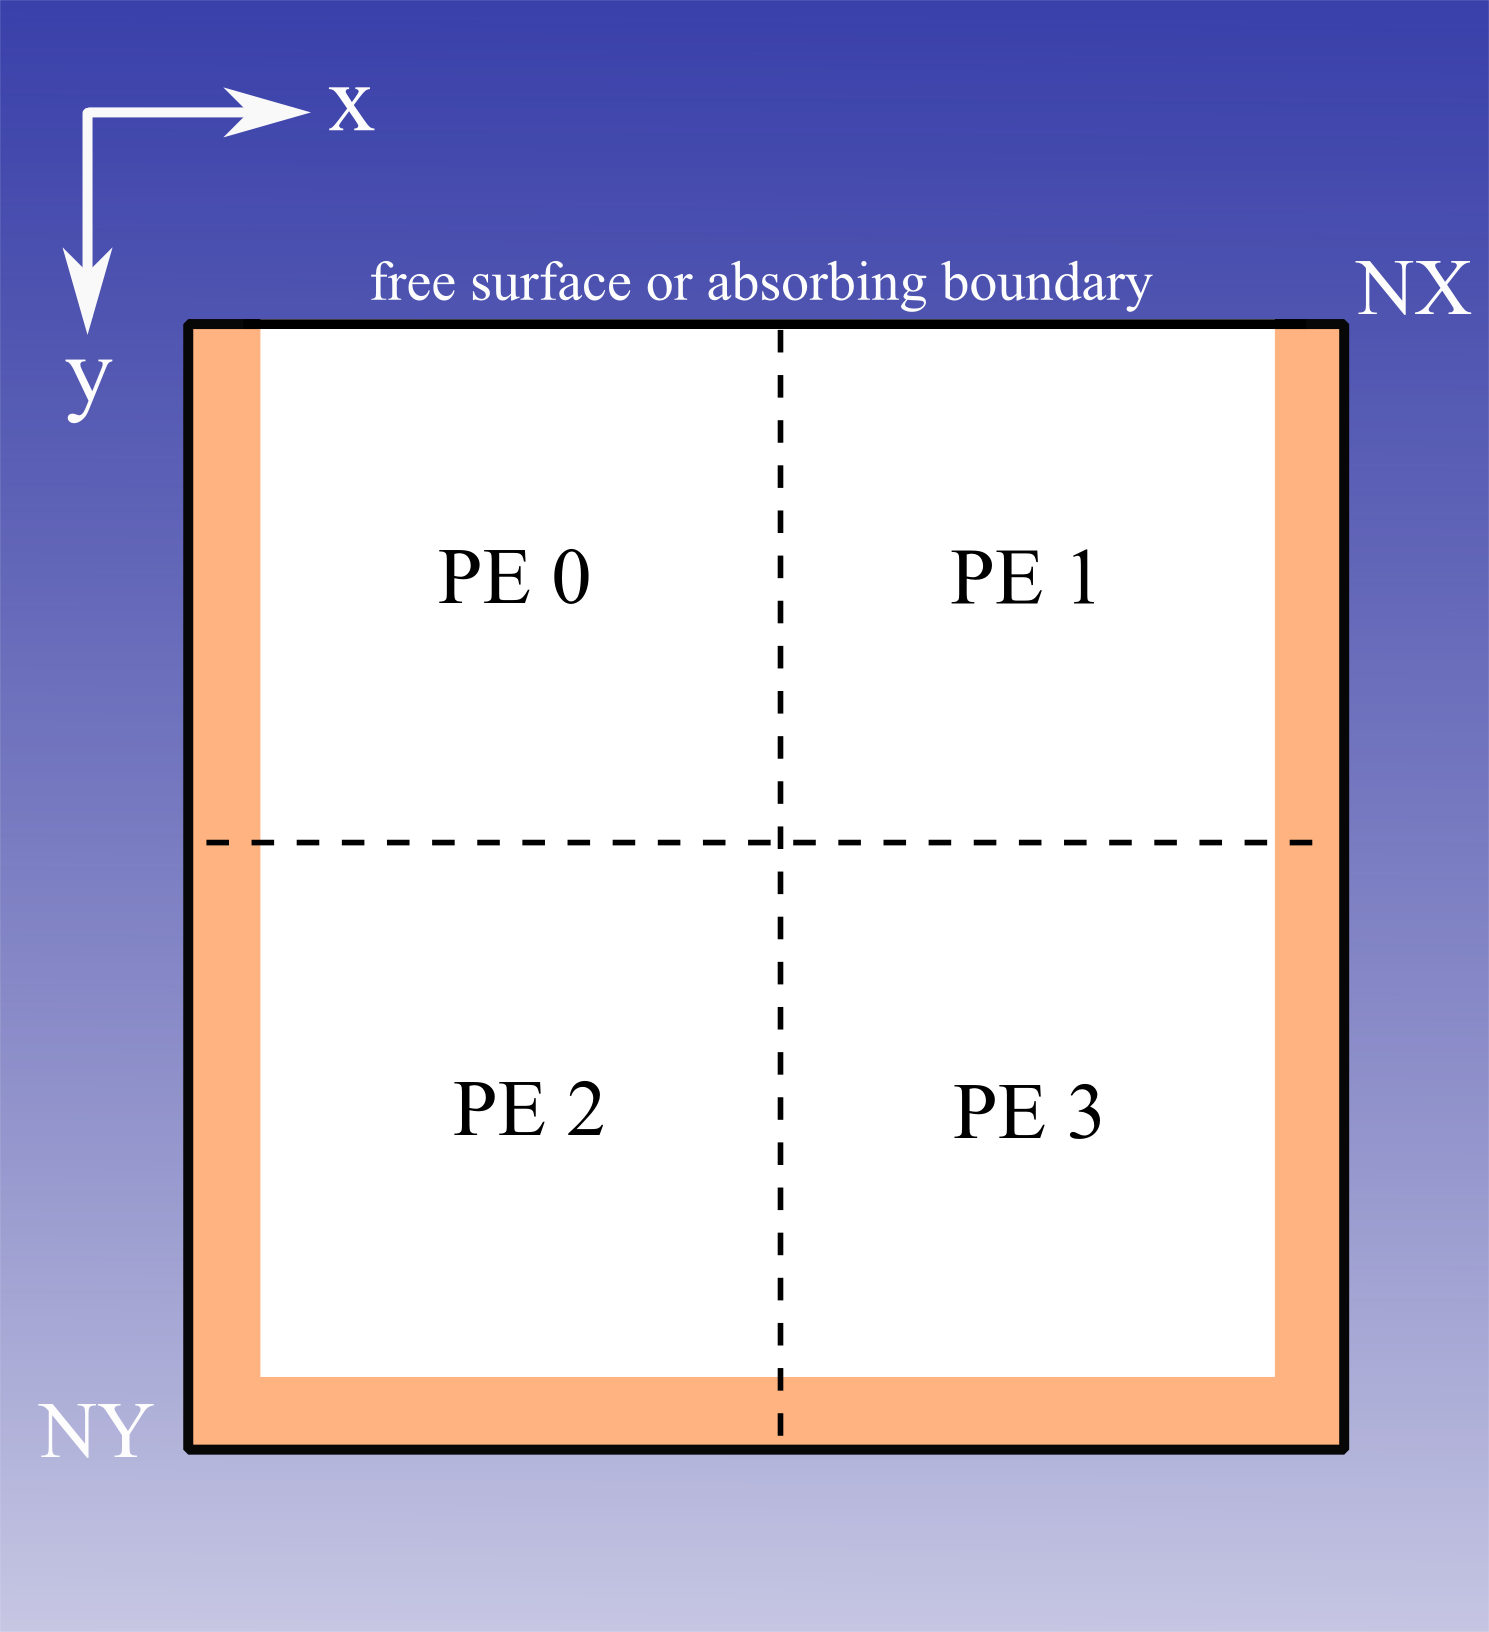
\includegraphics[width=7cm,angle=0]{figures/sketch_grid.png}
\end{center}
\caption{Geometry of the numerical FD grid using 2 processors in x-direction (NPROCX=2) and 2 processors in y-direction (NPROCY=2). Each processing element (PE) is updating the wavefield in its domain.
At the top of the numerical mesh the PEs apply a free surface boundary condition if FREE\_SURF=1, otherwise an absorbing boundary condition (PML). The width of the absorbing frame is FW grid points.  The size of the total grid is NX grid points in x-direction and NY gridpoints in y-direction. The size of each sub-grid  thus is NX/NPROCX x NY/NPROCY gridpoints. The origin of the Cartesian coordinate system (x,y) is at the top left corner of the grid.}
\label{fig_grid_json}
\end{figure}

\FloatBarrier
\newpage


\section{Order of the FD operator}
{\color{blue}{\begin{verbatim}
"FD order" : "comment",
			"FDORDER" : "2",
			"MAXRELERROR" : "0",
\end{verbatim}}}
The order of the used FD operator is defined by the option FDORDER (FDORDER=2,\,4\,6 or 8). With the option MAXRELERROR the user can switch between Taylor (MAXRELERROR=0) and Holberg (MAXRELERROR=1-4) FD coefficients of different accuracy. The chosen FD operator and FD coefficients have an influence on the numerical stability and grid dispersion (see chapter \ref{grid-dispersion}).

\section{Discretization}
{\color{blue}{\begin{verbatim}
"2-D Grid" : "comment",
			"NX" : "500",
			"NY" : "100",
			"DH" : "0.2",
\end{verbatim}}}
These lines specify the size of the total numerical grid (Figure  \ref{fig_grid_json}). NX and NY give the number of grid points in the x- and y-direction, respectively, and DH specify the grid spacing in x- and y-direction. The size of the total internal grid in meters in x-direction is NX*DH and in y-direction NY*DH. To allow for a consistent domain decomposition NX/NPROCX and NY/NPROCY must be integer values.

To avoid numerical dispersion the wavefield must be discretized with a certain number of gridpoints per wavelength. The number of gridpoints per wavelength required, depends on the order of the spatial
FD operators used in the simulation (see section \ref{grid-dispersion}). In the current FD software, 2nd, 4th, 6th and 8th order operators are implemented. The criterion to avoid numerical dispersion reads:
\begin{equation}
DH\le\frac{v_{s,\text{min}}}{2 f_c n} \label{eq_dispersion_json}
\end{equation}
where $\frac{v_{s,\text{min}}}{2 f_c}$ is the smallest wavelength propagating through the model and $v_{s,\text{min}}$ denotes the minimum shear wave velocity in the model, and $f_c=1/TS$ is the center frequency of the source wavelet. The program assumes that the maximum frequency of the source signal is approximately two times the center frequency. The center frequency is approximately one over the duration time TS. The value of n for different FD operators is tabulated in table \ref{grid_disp.2}. The criterion \ref{eq_dispersion_json} is checked by the FD software. If the criterion is violated a warning message will be displayed in the IFOS2D output section ``--- CHECK FOR GRID DISPERSION ---``. Please note, that the FD-code will NOT terminate due to grid dispersion, only a warning is given in the output file.


\section{Time stepping}
{\color{blue}{\begin{verbatim}
"Time Stepping" : "comment",
			"TIME" : "0.5",
			"DT" : "5.0e-05",
\end{verbatim}}}
The propagation time of seismic waves in the entire model is TIME (given in seconds). The time stepping interval (DT in s) has to fulfill the stability criterion \ER{courandt:1} in section \ref{courandt}. 
The program checks these criteria for the entire model, outputs a warning message if these are violated , stops the program and will output the time step interval for a stable model run. 

\newpage


\section{Sources}
\label{sec:sources}
{\color{blue}{\begin{verbatim}
"Source" : "comment",
			"SOURCE_SHAPE" : "4",
			"SOURCE_SHAPE values: ricker=1;fumue=2;from_SIGNAL_FILE=3;SIN**3=4;
			Gaussian_deriv=5;Spike=6;from_SIGNAL_FILE_in_su_format=7" : "comment",
			"SIGNAL_FILE" : "./ormsby.dat",
			
			"SOURCE_TYPE" : "3",
			"SOURCE_TYPE values (point_source): explosive=1;force_in_x=2;force_in_y=3;
			rotated_force=4" : "comment",
			
			"SRCREC" : "1",
			"SRCREC values : read source positions from SOURCE_FILE=1,
			 PLANE_WAVE=2" : "comment",
			 
			"SOURCE_FILE" : "./source/sources.dat",
			"RUN_MULTIPLE_SHOTS" : "1",
			
			"PLANE_WAVE_DEPTH" : "0.0",
			"PHI" : "0.0",
			"TS" : "0.032",
\end{verbatim}}}

{\color{red}{\begin{verbatim}
Default values are:
	SRCREC=1
\end{verbatim}}}

Five built-in wavelets of the seismic source are available. The corresponding source time functions are defined in \texttt{src/wavelet.c}. You may modify the time functions in this file and recompile to include your
own analytical wavelet or to modify the shape of the built-in wavelets.
\newline

SOURCE\_SHAPE=1, Ricker wavelet:
\begin{equation}
r(\tau)=\left(1-2\tau^2\right)\exp(-\tau^2) \quad \mbox{with} \quad \tau=\frac{\pi(t-1.5/f_c-t_d)}{1.0/f_c}
\label{eq_ricker}
\end{equation}

SOURCE\_SHAPE=2, Fuchs-M\"uller wavelet:
\begin{equation}
f_m(t)=\sin(2\pi(t-t_d)f_c)-0.5\sin(4\pi(t-t_d)f_c) \quad \mbox{if} \quad t\in[t_d,t_d+1/fc] \quad \mbox{else} \quad fm(t)=0
\label{eq_fm}
\end{equation}

SOURCE\_SHAPE=4, $sin^3$ wavelet:
\begin{equation}
s3(t)=0.75 \pi f_c \sin(\pi(t+t_d)f_c)^3\quad \mbox{if} \quad t \in[t_d,t_d+1/fc] \quad \mbox{else} \quad s3(t)=0
\label{eq_s3}
\end{equation}

SOURCE\_SHAPE=5, First derivative of a Gaussian function:
\begin{equation}
f(t)= -2.0 a (t-t_s) \exp(-a (t-t_s)^2)\quad \mbox{with} \quad a=\pi^2 f_c^2 \quad \mbox{and} \quad t_s=1.2/f_c
\label{eq_deriv_of_gaussian}
\end{equation}

SOURCE\_SHAPE=6, delta pulse: Lowpass filtered delta pulse. Note, that it is not clear if the lowpass filter used in the current version works correctly for a delta pulse.\\

% Source time function from SIGNAL\_FILE in su format (SOURCE\_SHAPE=7).\\

In these equations, t denotes time and $f_c$ is the center frequency. $t_d$ is a time delay which can be defined for each source position. Note that the symmetric (zero phase) Ricker signal is always delayed by $1.0/f_c$, which means that after one period the maximum amplitude is excited at the source location. Three of these 5 source wavelets and the corresponding amplitude spectra for a center frequency of $f_c=50$ Hz and $t_d=0$ are plotted in Figure \ref{fig_source_wavelets_json}. Note the delay of the Ricker signal described above. The Fuchs-M\"uller wavelet has a slightly higher center frequency and covers a broader frequency range.
\newline

\begin{figure}
\begin{center}
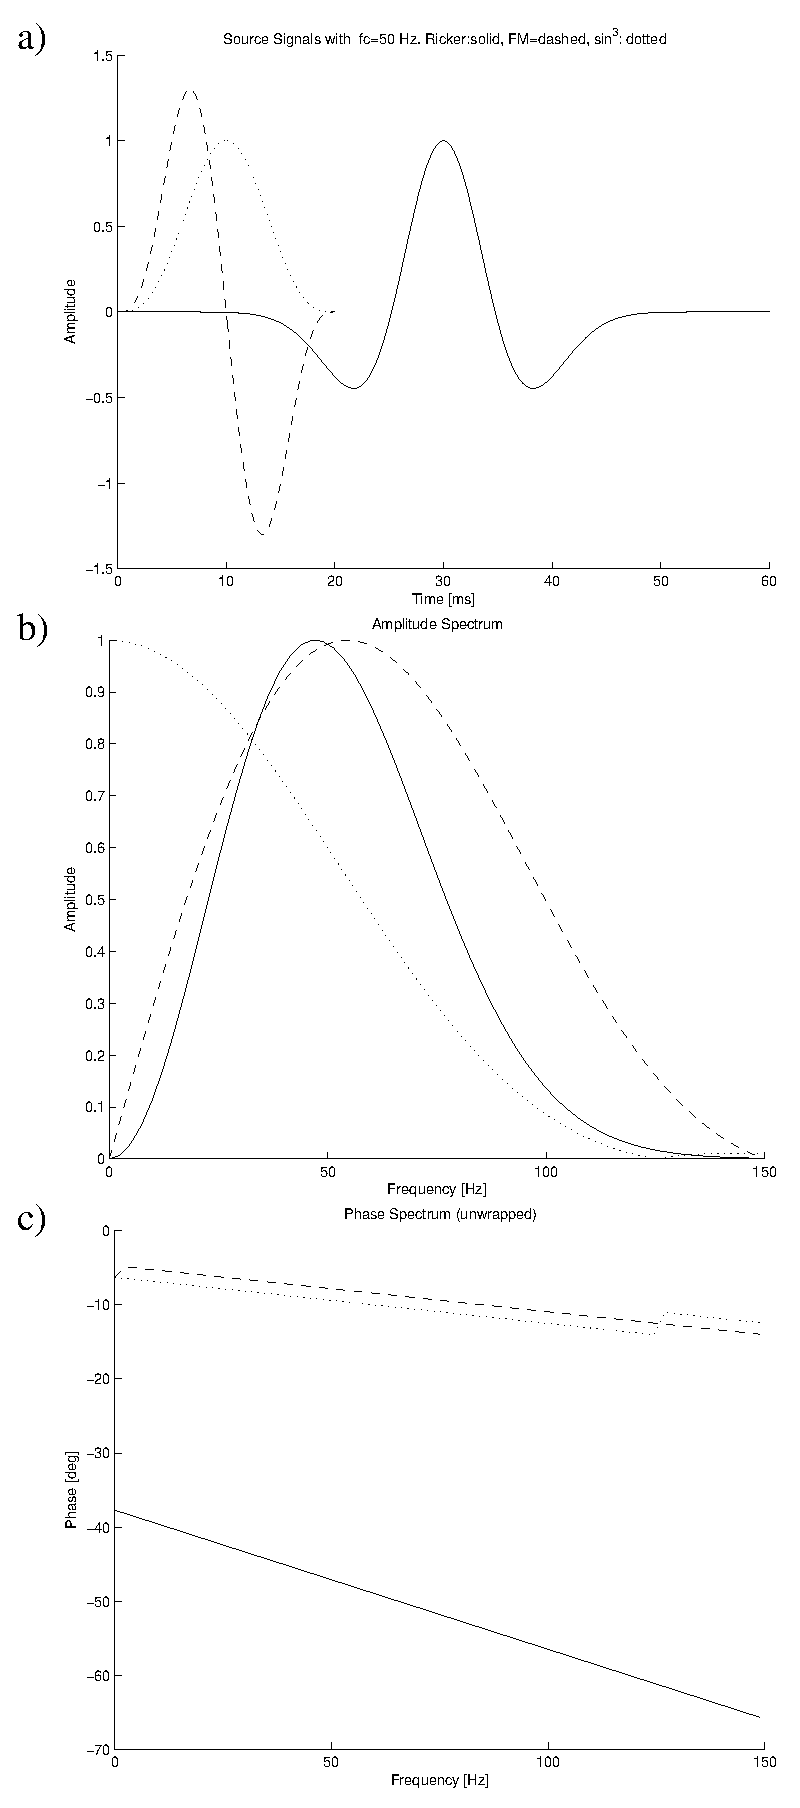
\includegraphics[width=8cm,angle=0]{figures/signals.eps}
\end{center}
\caption{Plot of built-in source wavelets (equations \ref{eq_ricker}, \ref{eq_fm}, \ref{eq_s3}) for a center frequency of $f_c=50$ Hz 
($TS=1/f_c=0.02$s): Ricker signal (solid), Fuchs-M\"uller signal (dashed), $sin^3$-signal (dotted). a) Time function, b) amplitude
spectrum, c) phase spectrum.  }
\label{fig_source_wavelets_json}
\end{figure}

\newpage

SOURCE\_SHAPE=3 allows you to use your own time function as the source wavelet stored in ASCII-format in SIGNAL\_FILE. SIGNAL\_FILE should then contain one sample per line. It should thus look like:

{\color{blue}{\begin{verbatim}
0.0
0.01
0.03
...
\end{verbatim}}}

The time interval between the samples must equal the time step interval (DT) of the FD simulation (see above)! Therefore it might be necessary to resample/interpolate a given source time function with a smaller sample rate. You may use the matlab script mfiles/resamp.m to resample your external source signal to the required sampling interval.
\newline

SOURCE\_SHAPE=7 is used for reading different external source wavelets for each shot. The wavelets in SU-format need to be saved in SIGNAL\_FILE.shot<shotnumber>.su.

If you want to use the source time function inversion (INV\_STF==1, section \ref{sec:STF}) with an external wavelet, this wavelet needs to be provided at SIGNAL\_FILE.shot<shotnumber>\_start.su and the inverted wavelets will be stored in SIGNAL\_FILE.shot<shotnumber>.su (or SIGNAL\_FILE.<workflowstage>.<shotnumber>.su if you use the WORKFLOW option).

The wavelets in each su file must have the same number of samples as specified by TIME/DT!
\newline

The following source types are availabe: explosive sources that excite compressional waves only (SOURCE\_TYPE=1), and point forces in the x- and y-direction (SOURCE\_TYPE=2,3).
The force sources excite both P- and S-waves. The explosive source is located at the same position as the diagonal elements of the stress tensor, i.e. at (i,j) (Figure \ref{fig_cell}).
The forces are located at the same position as the corresponding components of particle velocity (Figure \ref{fig_cell}). If (x,y) denotes the position at which the source location is defined in source.dat, then the actual force in x-direction is located at (x+DX/2,y) and the actual force in y-direction is located at (x,y+DY/2). With SOURCE\_TYPE=4 a custom directive force can be defined by a force angle between y and x. The angle of the force must be specified in the SOURCE\_FILE after AMP. This force is not aligned along the main directions.
\newline

The locations of multiple sources must be defined in an external ASCII file (SOURCE\_FILE) that has the following format:
{\color{blue}{\begin{verbatim}
NSRC
  % 	XSRC		ZSRC		YSRC		TD		FC		AMP  	SOURCE_AZIMUTH		SOURCE_TYPE	(NSRC lines)
\end{verbatim}}}

In the following lines, you can define certain parameters for each source point:\\
The first line must be the overall number of sources (NSRC). XSRC is the x-coordinate of a source point (in meter), YSRC is the y-coordinate of a source point (in meter). ZSRC is the z-coordinate should always be set to 0.0, because IFOS2D is a 2D code. TD is the excitation time (time-delay) for the source point (in seconds), FC is the center frequency of the source signal (in Hz), and AMP is the maximum amplitude of the source signal.
\newline

\textbf{Optional parameter:} The SOURCE\_AZIMUTH if SOURCE\_TYPE is 4. The SOURCE\_AZIMUTH is the angle between the y- and x-direction in degree and with SOURCE\_TYPE if SOURCE\_TYPE is set here, the value of SOURCE\_TYPE in the input file is ignored.

The SOURCE\_FILE = ./sources/source.dat that defines an explosive source  at $x_s=2592.0\;$ m and $y_s=2106.0\;$ m with
a center frequency of 5 Hz (no time delay) is
{\color{blue}{\begin{verbatim}
	2592.0        0.0        2106.0        0.0           5.0           1.0
\end{verbatim}}}

If the option RUN\_MULTIPLE\_SHOTS=0 in the parameter file all shot points defined in the SOURCE\_FILE are excitated simultaneously in one simulation. Setting RUN\_MULTIPLE\_SHOTS=1 will start individual model runs from i=1 to i=NSRC with source locations and properties defined at line i of the SOURCE\_FILE. (To apply a full waveform inversion you have to use RUN\_MULTIPLE\_SHOTS=1.) 

% Instead of a single source or multiple sources specified in the SOURCE\_FILE, you can also specify to excite a plane wave parallel (or tilted by an angle PHI) to the top of the model. This plane wave is approximated by a plane of single sources at every grid point at a depth of PLANE\_WAVE\_DEPTH below. The center source frequency $f_c$ is specified by the inverse of the duration of the source signal TS. SOURCE\_SHAPE and SOURCE\_TYPE are taken from the parameters as described above. If you choose the plane wave option by specifying a PLANE\_WAVE\_DEPTH$>$0, the parameters SRCREC and SOURCE\_FILE will be ignored.
% 
% This option will not be supported in future releases of IFOS2D.    

\newpage


\section{Acoustic Modelling}
\label{ac_mod}
{\color{blue}{\begin{verbatim}
"Acoustic Computation" : "comment",
			"ACOUSTIC" : "1",
\end{verbatim}}}

{\color{red}{\begin{verbatim}
Default value is:
	ACOUSTIC=0
\end{verbatim}}}

With this option pure acoustic modelling and/or inversion can be performed (ACOUSTIC = 1). Only a P-wave and a density model need to be provided. Acoustic modelling and inversion can be a quick estimate, especially for marine environments.

For acoustic modelling the option VELOCITY is not available and only PARAMETERIZATION = 1 is possible.

\section{PSV and SH modelling}
{\color{blue}{\begin{verbatim}
			"WAVETYPE" : "1",
\end{verbatim}}}

{\color{red}{\begin{verbatim}
Default value is:
	WAVETYPE=1
\end{verbatim}}}
In 2D the wave equations of PSV and SH waves are decoupled. Therefore the inversion problem is decoupled as well. With the variable WAVETYPE it is possible to switch between a PSV (WAVETYPE==1) and a SH (WAVETYPE==2) simulation. However the SH FWI is still in development and it is strongly recommended to use the PSV simulation. If ACOUSTIC is set to 1, WAVETYPE==1 will be enforced automatically.

\section{Model input}
\label{gen_of_mod}
{\color{blue}{\begin{verbatim}
"Model" : "comment",
			"READMOD" : "0",
			"MFILE" : "model/test",
\end{verbatim}}}

If READMOD=1, the P-wave, S-wave, and density model grids are read from external binary files. MFILE defines the basic file name that is expanded by the following extensions: P-wave model: ''.vp'', S-wave model: ''.vs'', density model: ''.rho''.  In the example above, the model files thus are: ''model/test.vp'' (P-wave velocity model),''model/test.vs'' (S-wave velocity model), and ''model/test.rho'' (density model). 

In these files, each material parameter value must be saved as 32 bit (4 byte) native float. Velocities must be in meter/second, density values in kg/m$^3$. The fast dimension is the y direction. See \texttt{src/readmod.c}. The number of samples for the entire model in the x-direction is NX, the number of values in the y-direction is NY. The file size of each model file thus must be NX*NY*4 bytes. You may check the model structure using the SU command ximage:
\newline

\textit{ximage n1=$<$NY$>$ $<$ model/test.vp} .
\newline

It is also possible to read Qp, and Qs grid files to allow for spatial variable attenuation. If no models are provided, the value TAU is used to generate Q-Models (see section \ref{q_approx}).

If READMOD=0 the model is generated ''on the fly'' by IFOS2D, i.e. it is generated internally before the time loop starts. See \texttt{genmod/1D\_linear\_gradient\_el.c} for an example function that generates a simple model with a linear vertical gradient ''on the fly''. If READMOD=0 this function is called in \texttt{src/IFOS2D.c} and therefore must be specified in \texttt{src/Makefile} (at the top of \texttt{src/Makefile}, see section \ref{compexec}). If you change this file, for example to change the model structure, you need to re-compile IFOS2D by changing to the src directory and ''make IFOS2D''.


\section{Free surface}  
{\color{blue}{\begin{verbatim}
"Free Surface" : "comment",
			"FREE_SURF" : "1",
\end{verbatim}}}
A plane stress free surface is applied at the top of the global grid if FREE\_SURF!=0 using the imaging method proposed by \cite{levander:88}. Note that the free surface is always located at $y$=0 or at the first grid point, respectively.


\section{Boundary conditions}
\label{abs}
{\color{blue}{\begin{verbatim}
"PML Boundary" : "comment",
			"FW" : "20",
			"VPPML" : "600.0",
			"FPML" : "31.25",
			"BOUNDARY" : "0",
			"npower" : "4.0",
			"k_max_PML" : "8.0",

\end{verbatim}}}
The boundary conditions are applied on each side face and the bottom face of the model grid. If FREE\_SURF = 0 the boundary conditions are also applied at the top face of the model grid. Note that the absorbing frames are always located INSIDE the model space, i.e. parts of the model structure are covered by the absorbing frame, in which no physically meaningful wavefield propagates. You should therefore consider the frame width when you design the model structure and the acquisition geometry (shot and receivers should certainly be placed outside).

A convolutional perfectly matched layer (CPML) boundary condition is used. The PML implementation is based on the following papers \cite{komatitsch:07} and \cite{martin:09}. A width of the absorbing frame of FW=10-20 grid points should be sufficient. For the optimal realization of the PML boundary condition you have to specify the dominant signal frequency FPML occurring during the wave simulation. This is usually the center source frequency FC specified in the source file. VPPML specifies the attenuation velocity in m/s within the PML. VPPML should be approximately the propagation velocity of the dominant wave near the model boundaries.

In some cases, it is usefull to apply periodic boundary conditions (see section \ref{bound_cond}). IF BOUNDARY=1 no absorbing boundaries are installed at the left/right sides of the grid. Instead, wavefield information is copied from left to right and vice versa. The effect is, for example, that a wave which leaves the model at the left side enters the model again at the right side.


\section{Receivers}
{\color{blue}{\begin{verbatim}
"Receiver" : "comment",
			"SEISMO" : "1",
			"READREC" : "1",
			"REC_FILE" : "./receiver/receiver.dat",
			"REFRECX, REFRECY" : "0.0 , 0.0",
			"XREC1, YREC1" : "6.0 , 0.2",
			"XREC2, YREC2" : "93.0 , 0.2",
			"NGEOPH" : "80",

\end{verbatim}}}

If SEISMO$>$0, seismograms are saved on hard disk. If SEISMO equals 1 x- and y-component of particle velocity will be written according to parameters specified in Chapter \ref{seismograms_json}.
If SEISMO = 2 pressure (sum of the diagonal components of the stress tensor) recorded at the receiver locations (receivers are hydrophones!) is written. If SEISMO = 3 the curl and divergence are saved. For SEISMO = 4 everthying is saved and for SEISMO = 5 everything except curl and divergence is saved.

The curl and divergence of the particle velocities are useful to separate between P- and S-waves in the snapshots of the wavefield. IFOS2D calculates the divergence and the magnitude of the curl of the particle velocity field according to \cite{dougherty:88}. The motivation for this is as follows. According to Morse and Feshbach \cite{morse:53} the energy of P- and S-wave particle velocities is, respectively,
\begin{equation}
E_p=\left(\lambda + 2 \mu\right) (div(\vec{v}))^2 \quad \mbox{and} \quad E_s=\mu \left|rot(\vec{v})\right|^2 \quad\mbox{.}
\label{eq_E}
\end{equation}
$\lambda$ and $\mu$ are the Lam\`{e} parameters, and $\vec{v}$ is the particle velocity vector.

The locations of the receivers may either be specified in a separate file REC\_FILE or in this parameter file. If READREC=1 receiver locations are read from the ASCII-file REC\_FILE. Each line contains the coordinates of one receiver, the first two number in each line indicate the horizontal x- and the vertical y-coordinate of each receiver position. To give an example of a receiver file, the following 3 lines specify 3 receivers located at constant depth (2106.0 m). However, the receiver coordinates change in x-direction (starting at 540 m) and therefore lining up along the x-axis. 
{\color{blue}{\begin{verbatim}
540.0   2106.0
1080.0  2106.0
1620.0  2106.0
\end{verbatim}}}
These receiver coordinates in REC\_FILE are shifted by REFREC[1], REFREC[2] into the  x- and y-direction, respectively. This allows for completely moving the receiver spread without modifying REC\_FILE. This may be useful for the simulation of moving profiles in reflection seismics.

If READREC=0 the receiver locations must be specified in the parameter file. In this case, it is assumed that the receivers are located along a straight line. The first receiver position is defined by (XREC1, YREC1), and the last receiver position by (XREC1, YREC1). The spacing between receivers is NGEOPH grid points. 

Receivers are always located on full grid indices, i.e. a receiver that is located between two grid points will be shifted by the FD program to the closest next grid point. It is not yet possible
to output seismograms for arbitrary receiver locations since this would require a certain wavefield interpolation.

\textbf{It is important to note that the actual receiver positions defined in REC\_FILE or in IFOS2D.json may vary by DH/2 due to the staggered positions of the particle velocities and stress tensor components. }

In our example, we specify 100 receiver location. Due to the small size of the model, most of the specified receiver positions will be located inside this absorbing boundary (if ABS=2, see Chapter \ref{abs}). A corresponding warning message will appear. If you choose to read the receiver location from REC\_FILE receiver.dat (READREC=1), only 10 receivers locations are considered. The list of receivers specified in file receiver.dat is equivalent to the parameters in the input file with only a larger distance between adjacent receivers (NGEOPH = 10.)


\section{Seismograms}
\label{seismograms_json}
{\color{blue}{\begin{verbatim}
"Seismograms" : "comment",
			"NDT" : "1",
			"SEIS_FORMAT" : "1",
			"SEIS_FILE" : "su/IFOS2D",
\end{verbatim}}}

{\color{red}{\begin{verbatim}
Default values are:
	NDT=1
\end{verbatim}}}

If SEISMO$>$0 seismograms recorded at the receiver positions are written to the corresponding output files. The sampling rate of the seismograms is NDT*DT seconds. In case of a small time step interval and a high number of time steps, it might be useful to choose a high NDT in order to avoid a unnecessary detailed sampling of the seismograms and consequently large files of seismogram data. Possible output formats of the seismograms are SU, ASCII and BINARY. It is recommended to use SU format for saving the seismograms. The main advantage of this format is that the time step interval (NDT*DT) and the acquisition geometry (shot and receiver locations) are stored in the corresponding SU header words. Also additional header words like offset are set by IFOS2D. This format thus facilitates a further visualization and processing of the synthetic seismograms. Note, however, that SU cannot handle sampling rates smaller than 1.0e-6 seconds and the number of samples is limited to about 32.000. In such cases, you should increase the sampling rate by increasing NDT. If this is impossible (for example because the Nyquist criterion is violated) you must choose a different output format (ASCII or binary). File endings will be added to SEIS\_FILE automatically. 


\section{Q-approximation}
\label{q_approx}
{\color{blue}{\begin{verbatim}
"Q-approximation",
			"L" : "0",
			"FL1" : "50.0", 
			"FL2" : "100.0",
			"TAU" : "0.00001",
			"F_REF" : "100",

\end{verbatim}}}

{\color{red}{\begin{verbatim}
Default values are:
	L=0
\end{verbatim}}}

These lines may be used to define an overall level of intrinsic (viscoelastic) attenuation of seismic waves. In case of L=0, a purely elastic simulation is performed (no absorption). The frequency dependence of the (intrinsic) Quality factor $Q(\omega)$ is defined by the L relaxation frequencies (FL=$f_l=2\pi/\tau_{\sigma l}$) and one value $\tau$ (see equation 5 in \cite{bohlen:02}). For a single relaxation mechanism (L=1) $Q \approx 2/\tau$ \citep{bohlen:98,blanch:95,bohlen:02}. If the model is generated ''on the fly'' the value of TAU can be assigned to all gridpoints for both P- and S-waves. Thus, intrinsic attenuation is homogeneous and equal for P- and S-waves ($Q_p(\omega)=Q_s(\omega)$). However, it is possible to simulate any spatial distribution of absorption by assigning the gridpoints with different Q-values by reading external grid files for $Q_p$ (P-waves) and $Q_s$ (S-waves) (see \texttt{src/readmod.c}) or by generating these files ''on the fly'' (see section \ref{gen_of_mod} or exemplary model function \texttt{genmod/1D\_linear\_gradient\_visc.c}).  

Small $Q$ values ($Q<50$) may lead to significant amplitude decay and velocity dispersion. Please note, that due to dispersive media properties the viscoelastic velocity model is defined for the reference frequency only. In IFOS2D, this reference frequency is specified as the center source frequency. With F\_REF one can set the reference frequency manually. At the exact reference frequency, elastic and viscoelastic models are equivalent. As a consequence, slightly smaller and larger minimum and maximum velocity values occure in the viscoelastic model.

The frequency dependence of attenuation, i.e. $Q$ and phase velocity as a function  of frequency, may be calculated using the Matlab functions in the directory mfiles. The Matlab script /mfiles/qplot.m can be used to plot $Q(\omega)$ for different values of L, $f_l$ and $\tau$. The m-file qapprox.m in the same directory finds optimal values for L, $f_l$ and $\tau$ that fit a desired function $Q(\omega)=const$ in a least-squares sense.


\section{Wavefield snapshots}
{\color{blue}{\begin{verbatim}
"Snapshots" : "comment",
			"SNAP" : "0",
			"TSNAP1" : "2.7e-3",
			"TSNAP2" : "6.0",
			"TSNAPINC" : "0.12",
			"IDX" : "1",
			"IDY" : "1",
			"SNAP_FORMAT" : "3",
			"SNAPSHOT_START , SNAPSHOT_END , SNAPSHOT_INCR" : "2, 3 , 2",
			"SNAP_FILE" : "./snap/waveform_forward",
\end{verbatim}}}

{\color{red}{\begin{verbatim}
Default values are:
SNAP=0
IDX=1
IDY=1
\end{verbatim}}}

If SNAP$>0$, wavefield information (particle velocities (SNAP=1), pressure (SNAP=2), or curl and divergence of particle velocities (SNAP=3), or everything (SNAP=4)) for the entire model is saved on the hard disk (assure that enough free space is on disk!). Each PE is writing his sub-volume to disk. The filenames have the basic filename SNAP\_FILE plus an extension that indicates the PE number in the logical processor array (SNAP\_FILE.<PEnumber>). The first snapshot is written at TSNAP1 seconds of seismic wave traveltime to the output files, the second at TSNAP1 + TSNAPINC seconds etc. The last snapshots contains wavefield at TSNAP2 seconds. With SNAPSHOT\_START (SNAPSHOT\_END) you can specify the first (last) shot, for which a snapshot should by generated. The increment for the shotwise output of the snapshots can be defined in the variable SNAPSHOT\_INCR. Note that the file sizes increase during the simulation. The snapshot files might become quite LARGE. It may therefore be necessary to reduce the amount of snapshot data by increasing IDX, IDY and/or TSNAPINC. In order to merge the separate snapshots of each PE after the completion of the wave modeling, you can use the program snapmerge (see Chapter \ref{installation}, section \textbf{src}). The bash command line to merge the snapshot files can look like this: 
\newline

\textit{../bin/snapmerge IFOS2D.json}.


\section{Monitoring the simulation}
{\color{blue}{\begin{verbatim}
"Monitoring the simulation" : "comment",
			"LOG_FILE" : "log/2layer.log",
			"LOG" : "1",
\end{verbatim}}}

{\color{red}{\begin{verbatim}
Default values are:
LOG=1
LOG_FILE="log/LOG_FILE"
\end{verbatim}}}

IFOS2D can output a lot of useful information about the modeling parameters and the status of the modeling process etc. The major part of this information is output by PE 0.
If LOG=1, PE 0 writes this info to stdout, i.e. on the screen of your shell. This is generally recommended to monitor the modeling process. You may want to save this screen info to an output file by adding ''$>$ IFOS2D.out'' or ''| tee IFOS2D.out''. to your starting command. If LOG=1 all other processes with PE number greater than zero will write their information to LOG\_FILE.<PEnumber>. If you specify LOG=2 PE 0 will also output information to LOG\_FILE.0. As a consequence only little information is written directly to the screen of your shell. On supercomputers where you submit modeling jobs to a queuing system as batch jobs LOG=2 may be advantageous. In case of LOG=2, you may still watch the simulation by checking the content of LOG\_FILE.0 for example by using the Unix commands more or tail. After finishing the program the timing information is written to the ASCII file log/test.log.0.timings. This feature is useful to benchmark your local PC cluster or supercomputer. If LOG=0 no output from node 0 will be written, neither to stdout nor to an LOG file. There will be also no output of timing information to the ASCII file log/test.log.0.timings.
If TIME\_FILT is set to one the log file L2\_LOG.dat contains a 9th column with the corner frequency in Hz used in the iteration step.

\newpage


\section{General inversion parameters}
{\color{blue}{\begin{verbatim}
"General inversion parameters" : "comment",
			"ITERMAX" : "10",
			"DATA_DIR" : "su/measured_data/IFOS2D_real",
			"PARAMETERIZATION" : "1",
			"FORWARD_ONLY" : "0",
			"ADJOINT_TYPE" : "1",
			"MISFIT_LOG_FILE" : "L2_LOG.dat",
			"VELOCITY" : "0",

"Inversion for ..." : "comment",
			"INV_RHO_ITER" : "0",
			"INV_VP_ITER" : "0",
			"INV_VS_ITER" : "0",
\end{verbatim}}}

{\color{red}{\begin{verbatim}
Default values are:
MISFIT_LOG_FILE=L2_LOG.dat
VELOCITY=0
INV_RHO_ITER=0
INV_VP_ITER=0
INV_VS_ITER=0
\end{verbatim}}}

This section covers some general inversion parameters. The maximum number of iterations is defined by ITERMAX. The switch FORWARD\_ONLY controls if only the forward modeling code should be used (FORWARD\_ONLY=1), e.\,g. to calculate synthetic seismograms or a complete FWT run (FORWARD\_ONLY=0). The seismic sections of the real data need to be located in DATA\_DIR and should have the ending \_vx.su.shot<shotnumber> for the x-component and so on. As noted in section \ref{model parametrizations} the gradients can be expressed for different model parameterizations. The switch PARAMETERIZATION defines which parameterization should be used, seismic velocities and density (Vp,Vs,rho, PARAMETERIZATION=1), seismic impedances (Zp,Zs,rho, PARAMETERIZATION=2) or Lam$\rm{\acute{e}}$ parameters ($\rm{\lambda,\mu,\rho}$, PARAMETERIZATION=3). Please use PARAMETERIZATION>1 with care, as current developers are only working with PARAMETERIZATION=1.

If models are read from binary files appropriate file extensions are required for the different models (see section \ref{gen_of_mod}). Depending on the data different components of the seismic sections can be back propagated. For two component data (x- and y-component) set ADJOINT\_TYPE=1, only the y-component (ADJOINT\_TYPE=2) and only the x-component (ADJOINT\_TYPE=3). For the inversion of pressure seismograms ADJOINT\_TYPE=4 has to be used.

During the inversion the misfit values are saved in a log file specified in MISFIT\_LOG\_FILE. The log file consists of eight or nine columns and each line corresponds to one iteration step. The used step length is written in the first column. In the second to fourth column the three test step lengths used for the step length estimation are saved. The corresponding misfit values for these test step lengthes and the test shots are written to column five to seven. Column eight corresponds to the total misfit for all shots and if you use frequency filtering then the ninth column corresponds to the corner frequency of the lowpass filter used in the inversion step.

In general IFOS2D tries to minimize the misfit in the particle displacement between the observed data and the synthetic data. If you set the switch VELOCITY to 1 the misfit in the particle velocity seismograms is minimized.

The parameters INV\_RHO\_ITER, INV\_VP\_ITER and INV\_VS\_ITER define from which inversion step on an inversion for density, Vp and Vs, respectively, is applied. To invert for one parameter from the beginning of an inversion set it to 0 or 1.


\section{Output of inversion results}
\label{sec:Output_of_inversion_results_json}
{\color{blue}{\begin{verbatim}
"Output of inverted models" : "comment",
			"INV_MODELFILE" : "model/model_Test",
			"nfstart" : "1",
			"nf" : "1",

"Output of gradients" : "comment",
			"JACOBIAN" : "jacobian/jacobian_Test",
			"nfstart_jac" : "1",
			"nf_jac" : "1",
\end{verbatim}}}

The inverted models are saved in INV\_MODELFILE. The first model that is saved is at iteration step nfstart and then every $\mathrm{nf}^{\mathrm{th}}$ iteration step. Analog the gradients are saved every $\mathrm{nf\_jac}^{\mathrm{th}}$ iteration step from iteration step nfstart\_jac on in JACOBIAN. 

\section{Workflow}
\label{sec:workflow}
{\color{blue}{\begin{verbatim}
"Workflow" : "comment",
			"USE_WORKFLOW" : "1",
			"FILE_WORKFLOW" : "workflow.txt",
\end{verbatim}}}
{\color{red}{\begin{verbatim}
Default values are:
"USE_WORKFLOW" : "0"
\end{verbatim}}}
With the use of a workflow file, you can define different FWI stages. For instance, one FWI stage could refer to one corner frequency of a low-pass filter or to a specific time window. Every line in the workflow file corresponds to one FWI stage. To use a workflow file the switch USE\_WORKFLOW have to be set to 1.  The algorithm will automatically change to the next line of the workflow file if the abort criterium of the current line is reached or if no step length could be found which reduces the misfit. The structure of the variables inside the workflow file is as follow: \\

\noindent
\begin{tabular}{llllllllllll}
\# & INV\_VS & INV\_VP & INV\_RHO & PRO & TIME\_FILT & FC & WAVETYPE & 0 & 0 & EPRECOND & EPSILON\_WE\\
\end{tabular}

\ \\
The first column is the number of the line. With INV\_* etc. you can activate the inversion for VS, VP or RHO, respectively. The abort criterium in percent for this FWI stage will be the declared in the variable PRO. With TIME\_FILT you can activate the frequency filtering with the corner frequency FC. WAVETYPE can be used to switch between PSV and SH modeling, however it is recommended to use PSV modeling (WAVETYPE==1) due to the current development on SH modeling. The following to zeros are placeholders for an upcoming update. With EPRECOND and EPSILON\_WE you can control the approx. Hessian. Please note, that all features which are used eg. TIME\_FILT (see section \ref{sec:filtering}) within the workflow have to be activated in the .JSON file.

For an example of a workflow file, have a look in the par/ folder.


\section{Approx. Hessian preconditioning}
{\color{blue}{\begin{verbatim}
			"EPRECOND" : "3",
			"EPSILON_WE" : "0.005",
			
			"EPRECOND_PER_SHOT" : "1",
\end{verbatim}}}
{\color{red}{\begin{verbatim}
Default values are:
			"EPRECOND" : "0",
\end{verbatim}}}

With the variable EPRECOND it is possible to activate an approximated Hessian for preconditioning. There are two different approximations available. EPRECOND==1 will be an approximation after \cite{shin2001efficient}, and EPRECOND==3 after \cite{plessix2004frequency}. EPSILON\_WE defines a water level to stabilize the approximated Hessian. The use of an approximated Hessian can significantly influence the speed of convergence. The Hessian is calculated for each shot individually and will be applied to the gradient from each shot directly if the switch EPRECOND\_PER\_SHOT is set to 1. Otherwise (EPRECOND\_PER\_SHOT==0) the Hessian will be summed up for each shot and will be applied to the total gradient. 
Up to now there is no rule of tumb wether EPRECOND==1 or ==3 should be chosen,  so it is recommended to try both. After each iteration the Hessian will be outputted in the folder JACOBIAN with the syntax \*approx\_hessian\* in the file name.\\
The corresponding functions are copied out of DENISE Black Edition, which is maintained by Daniel Koehn. 

\section{PCG and L-BFGS}
{\color{blue}{\begin{verbatim}
"Gradient-Method" : "comment",
			"GRAD_METHOD" : "2",
			"N_LBFGS" : "5",
			
			"WOLFE_CONDITION" : "1",
			"WOLFE_TRY_OLD_STEPLENGTH" : "1",
			"WOLFE_NUM_TEST" : "5", 
			"WOLFE_C1_SL" : "1e-4",
			"WOLFE_C2_SL" : "0.9",
			
			"LBFGS_STEP_LENGTH" : "0",
\end{verbatim}}}

{\color{red}{\begin{verbatim}
Default values are:
	"GRAD_METHOD" : "1",
\end{verbatim}}}

IFOS2D contains the option to chose between a preconditioned conjugate gradient (PCG) method or a quasi-newton L-BFGS method.

The preconditioned conjugate gradient (PCG), which can be used by GRAD\_METHOD==1, is very robust, however in general shows slow convergence. For a quick-and-dirty inversion or if you want to run an inversion without worry about a stable L-BFGS inversion it is recommended to use PCG, due to the higher stability and robustness of convergence.

The L-BFGS method is a quasi-newton method, which will implicitly approximate the Hessian and can be chosen by setting GRAD\_METHOD to 2. Therefore the differences of the models and the gradients of a N\_LBFGS last iterations will be stored. First tests showed that N\_LBFGS=10 should be enough. The L-BFGS algorithm is implemented after the book \cite{nocedal:1999}, which is recommended to be read prior to using the L-BFGS method. Prior to starting the L-BFGS method one update with steepest decent have to be done to get a first set of model and gradient differences which are necessary to start L-BFGS.

To ensure a stable convergence when L-BFGS is used the step length has to satisfy the wolf condition. A detailed description of the wolfe condition can be also found in \cite{nocedal:1999}. The first wolfe condition, which is also called sufficient decrease condition, requires that the misfit for a chosen step length will be decreased at least linear with the step length. Let $f(x)$ be the objective function, $x$ the current model, $\alpha$ the step length and $p$ the desired model update, so the first wolfe condition reads \citep{nocedal:1999}:
\begin{align}
	f(x+\alpha \cdot p) \le f(x) + c_1 \cdot \alpha \cdot\bigtriangledown f(x)^{T} \cdot p
\end{align}

The second one, which is called curvature condition, requires that the slope of the misfit function will be higher than the initial slope. This ensures that the next misfit minimum will be reached fast enough.
The second criterium is defined as \citep{nocedal:1999}:
\begin{align}
	\bigtriangledown f(x+\alpha \cdot p)^{T} \cdot p \geq c_2 \cdot\bigtriangledown f(x)^{T} \cdot p
\end{align}
To verify this condition the full gradient (with all shots!) of the updated model have to be calculated, so the verification of this condition is very expensive in terms of computation time. In theory always a step length of one should be tried first, however to save time it is possible to chose the step length from the iteration before which satisfied the Wolfe condition. This behavior can be controlled with WOLFE\_TRY\_OLD\_STEPLENGTH, if this is set to 1 always the old step length will be tried first. In practice the experience has shown that at the beginning of a FWI stage a couple of step lengths will be tested and then the algorithm converges to a step length which will be accepted by the Wolfe condition until the misfit cannot be reduced further. With the variable WOLFE\_NUM\_TEST a maximum number of test calculations can be defined. If after WOLFE\_NUM\_TEST tests no step length could be found, the algorithm takes the step length of the tests which reduced the misfit most, even if this step length does not satisfy the wolfe condition. If no step length was found which reduces the misfit, the algorithm will switch to the next FWI stage in the workflow file or abort the inversion. 
The variable $c_1$ will be $10^{-7}\cdot \max(f(x)^{-1}$ and $c_2$ is set to 0.9. With WOLFE\_C1\_SL and WOLFE\_C2\_SL it is possible to manipulate $c_1$ and $c_2$ with the JSON input file. If the parameters are not set, they will be set to default values, so in most cases it should be the best to do not specify theses parameters in the JSON file.
A step length search which is based on the Wolfe condition can be used which the switch WOLFE\_CONDITION. Please note that this step length search is only available if GRAD\_METHOD==2. 

However, it is possible to chose a second step length search while the L-BFGS method is used. This one is available by the switch LBFGS\_STEP\_LENGTH=0. If you use LBFGS\_STEP\_LENGTH the Wolfe condition based step length search will be deactivated automatically. With this search the step length 0.1, 0.5 and 1.0 will be tried and with a parabolic fit the best step length will be estimated. This search algorithm is implemented to save computation time, however the Wolfe condition will not be checked, so the L-BFGS stability will not be satisfied. It is \textbf{highly} recommended to use the step length search based on the Wolfe condition (LBFGS\_STEP\_LENGTH=1 and WOLFE\_CONDITION=1). Most likely the option LBFGS\_STEP\_LENGTH=0 will be removed in a future release. 


\section{Step length estimation}
{\color{blue}{\begin{verbatim}
"Step length estimation" : "comment", 
			"EPS_SCALE" : "0.01", 
			"STEPMAX" : "4",
			"SCALEFAC" : "4.0",
			"TESTSHOT_START , TESTSHOT_END , TESTSHOT_INCR" : "1 , 2 , 1",
\end{verbatim}}}

For the step length estimation a parabolic line search method proposed by \cite{sourbier:09,sourbier:09b}, \cite{brossier:2009} and \cite{nocedal:1999} is implemented. For this step length estimation only two further test forward modelings are needed. The vector L2t contains the misfit values and the vector epst contains the corresponding step length. During the forward modeling of an iteration step the misfit norm of the data residuals is calculated for the shots defined by  TESTSHOT\_START, TESTSHOT\_END and TESTSHOT\_INC. The value L2t(1) then contains the misfit from the forward modeling and the corresponding epst(1) value is 0.0.\\

The step lengths for the different parameters are defined as:\\
EPSILON = EPS\_SCALE * m\_max/grad\_max
EPSILON = epst[i] * m\_max/grad\_max\\
where m\_max is the maximum value of the corresponding model parameter in the whole model and grad\_max is the maximum absolute value of the gradient.\\

For a better definition of the parabola the improved line search is now trying to estimate a steplength epst(2) with L2t(2)<L2t(1). If the code is not able to find an appropiate steplength using the user-defined value EPS\_SCALE (f.e. EPS\_SCALE = 0.01 = 1\% change in terms of m\_max/grad\_max), the code divides this steplength by the variable SCALEFAC and calculates the misfit norm again. If this search fails after STEPMAX attempts IFOS2D exits with an error message. If the algorithm has found an appropriate value for epst(2), it is trying to estimate a steplength epst(3) with L2t(3)> L2t(2), by increasing the steplength\\

EPS\_SCALE += EPS\_SCALE/SCALEFAC.\\

If a corresponding value epst(3) can be found after STEPMAX forward modellings, IFOS2D can fit a parabola through the 3 points (L2t(i),epst(i)) and estimates an optimum step length at the minimum of the parabola. If the L2-value L2t(3) after STEPMAX forward models is still smaller than L2t(2) the optimum steplength estimated by parabolic fitting will be not larger than epst(3).\\

Please note: This step length search is only available wenn PCG method (GRAD\_METHOD==1) is used and will be automatically selected.


\section{Misfit definition}
{\color{blue}{\begin{verbatim}
"Misfit Definition" : "comment",
			"LNORM" : "2",
			"NORMALIZE" : "0",
			"DTINV" : "2",
			"WATERLEVEL_LNORM8" : "0.0",
\end{verbatim}}}

With LNORM=2 the L2 norm is used as misfit definition. In this case the misfit is scaled with the energy of the observed seismograms.\\
With LNORM=5 the global correlation is used as misfit function. It was suggested e.\,g. by \cite{choi:2012} and consists of a zero-lag cross correlation of two normalized signals. The misfit is calculated by
\begin{equation}
E = - \sum_i^{ns} \sum_j^{nr} \sum_k^{nc} \frac{\vec{u}_{i,j,k} \cdot \vec{d}_{i,j,k}}{|\vec{u}_{i,j,k}| |\vec{d}_{i,j,k}|}
\end{equation}
where the sum over $i$ denotes the sum over the sources, the sum over $j$ denotes the sum over the receivers and the sum over $k$ denotes the sum over the components used in the inversion. $\vec{u}$ are the forward modeled data and $\vec{d}$ are the observed data. The misfit is minimized but the misfit function is not yet normalized. Therefore, a perfect fit results in a misfit of $(-1)\cdot ns \cdot nr \cdot nc$.\\
LNORM=1 uses the L1 norm, LNORM=3 the Cauchy norm and LNORM=4 the SECH norm.\\
LNORM=7 uses the normalized L2 norm
\begin{equation}
 E=\frac{\sum_i^{ns} \sum_j^{nr} \sum_k^{nc} \left| \frac{\vec{u}_{i,j,k}}{|\vec{u}_{i,j,k}|}-\frac{\vec{d}_{i,j,k}}{|\vec{d}_{i,j,k}|}\right|^2}{\sum_i^{ns} \sum_j^{nr} \sum_k^{nc} \left| \frac{\vec{d}_{i,j,k}}{|\vec{d}_{i,j,k}|}\right|^2}
\end{equation}
 suggested by \cite{choi:2012}. The misfit is scaled with the energy of the observed seismograms.\\ 
LNORM=8 is based on an envelope-based objective function which compares the difference between the envelopes of observed and synthetic wave fields.
The misfit function is defined by
\begin{equation}
E= \frac{1}{2} \sum_i^{ns} \sum_j^{nr} \sum_k^{nc} \int_0^T \left( \text{env}(\vec{u}_{i,j,k}) - \text{env}(\vec{d}_{i,j,k}) \right)^2~\text{d}t.
\label{misfit_envelope}
\end{equation}
At time samples $t$ where the envelope of the synthetics $\text{env}( u)$ becomes small with respect to the noise of the observed data $\text{env}( d)$, the corresponding adjoint source develops a singularity (for $\text{env}( u) \rightarrow 0$). A finite water-level (WATERLEVEL\_LNORM8) is used to keep the division regular. The water-level is estimated about the smallest signal amplitude of the observed data which is considered in the misfit.\\
If NORMALIZE is set to 1, the synthetic data and the measured data will be normalized before calculating the residuals.\\

To reduce the memory requirements during an inversion one can define that only every DTINV time sample is used for the calculation of the gradients. To set this parameter appropriately one has to keep in mind the Nyquist criterion to avoid aliasing effects.


\section{Abort criterion}
\label{json:abort_criterion}
{\color{blue}{\begin{verbatim}
"Termination of the programmme" : "comment",
			"PRO" : "0.01",
\end{verbatim}}}
Additionally to the parameter ITERMAX a second abort criterion is implemented in IFOS2D which is using the relative misfit change within the last two iterations. The relative misfit of
the current iteration step and the misfit of the second to last iteration step is calculated with regard to the misfit of the second to last iteration step. If this relative change is
smaller than PRO the inversion aborts or in case of using frequency filtering (TIME\_FILT==1) it increases the corner frequency of the low pass filter and therefore switches to next higher bandwidth. 

\newpage

\section{Source wavelet inversion}
\label{sec:STF}
To remove the contribution of the unknown source time function (STF) from the waveform residuals, it is necessary to design a filter which minimizes the misfit to the field recordings and raw synthetics. Therefore, a second forward simulation is applied. The first one is done with the wavelet specified in SOURCE\_SHAPE and the second one with the optimized source wavelet saved in SIGNAL\_FILE (see Section~\ref{sec:sources}). This optimized source wavelet is kept constant within N\_STF or within a frequency range (see below).\\

{\color{blue}{\begin{verbatim}
"Definition of inversion for source time function" : "comment",
			"INV_STF" : "0",
			"PARA" : "fdlsq:exp=1.0",
			"N_STF" : "10",
			"N_STF_START" : "1",
			"TAPER_STF" : "0",
			
			"TRKILL_STF" : "0", 
			"TRKILL_FILE_STF" : "./trace_kill/trace_kill",
			
			"TRKILL_STF_OFFSET" : "0", 
			"TRKILL_STF_OFFSET_LOWER" : "10",
			"TRKILL_STF_OFFSET_UPPER" : "20",
			"TRKILL_STF_OFFSET_INVERT" : "0",
\end{verbatim}}}

{\color{red}{\begin{verbatim}
Default values are:
	INV_STF=0
\end{verbatim}}}

INV\_STF should be switched to 1 if you want to invert for the source time function.
\newline

An example for the parameter string provided in PARA is:
\begin{itemize}
 \item To select frequency domain least squares (fdlsq), apply offset dependent weights and a waterlevel use\\
 \textit{fdlsq:exp=1.0:waterlevel=0.01}
\end{itemize}

In most cases the frequency domain least squares engine is the best approach to find a suitable wavelet. There are also other possibilities, if you want to use those a detailed look at the libraries and the acompanying documentation provided in the folder /contrib is recommended. Here only the two main parameters for the fdlsq approach are described.

Due to the amplitude decay with offset to the source signals from receivers at larger offset would contribute less to the optimization criterion for which the source wavelet correction filter is constructed. The option exp=k provides means to add a weight factor $(r/1\text{m})^k$ to each signal, where r is the receiver to source offset. This is used to compensate the decrease in signal amplitude.

The procedure is implemented in the Fourier domain. Fourier coefficients for the correction filter are constructed such that the residual between Fourier coefficients of recorded signals and Fourier coefficients of synthetic signals after application of the correction filter are minimized in a least-squares sense. The least-squares solution is subject to a damping constraint. If the weighted power spectral density of the synthetics at a given frequency drops below the l-th fraction (waterlevel parameter) of the average (over all frequencies) power spectral density, the filter coefficients are damped (artificially made smaller) by the damping constraint (i.e. waterlevel as seen from the perspective of deconvolution). 

Start with l=0.01 as a reasonable initial value for the water-level. The best fitting water-level must be searched by trial and error and depends of signal noise and on how well the synthetics describe the actually observed wave propagation.

The theory behind the Fourier domain least squares procedure is outlined by Lisa Groos (2013, Appendix F, page 146). She also describes a way to find an appropriate water-level by application of the L-curve criterion (Groos, 2013, Appendix G, page 148).
\newline

N\_STF is the increment between the iteration steps. N\_STF\_START defines at which iteration-step the inversion for STF should start. This parameter has to be set at least to 1 NOT(!) 0. When using TAPER\_STF = 1, the source signal is tapered. See \texttt{src/taper.c} for the taper definition. With TRKILL\_STF = 1 it is possible to apply a trace killing for the estimation of the source wavelet correction filter. Similar as for the normal trace killing (see section \ref{sec:trace_killing}) it is possible to use an offset based trace kill. To use this one, TRKILL\_STF\_OFFSET and TRKILL\_STF have to be set one. Than all offsets between TRKILL\_STF\_OFFSET\_LOWER (in meter) and TRKILL\_STF\_OFFSET\_UPPER (in meter) will be killed. The offset is calculated internally for each source - receiver combination. If TRKILL\_STF\_OFFSET is set to two, the trace kill file and the offset based trace kill will be combined. Additionally, the option TRKILL\_STF\_OFFSET\_INVERT allows to invert the sense of the offset based trace kill for the STF inversion. If TRKILL\_STF\_OFFSET\_INVERT is set to one, all offsets which do not lie inside the specified range will be killed. This means, the specified offset range will work like a band pass. However, it is not possible to combine a trace kill file and the offset based trace kill, if you invert the sense of the offset based trace kill. \textit{Example}: If you only want to use an offset range from ten to 20 meters for the STF inversion, you would have to set TRKILL\_STF and TRKILL\_STF\_OFFSET to one, TRKILL\_STF\_OFFSET\_LOWER to ten, TRKILL\_STF\_OFFSET\_UPPER to 20 and TRKILL\_STF\_OFFSET\_INVERT to one.
\newline

Please note: If you additionally switch on frequency filtering during the inversion (TIME\_FILT=1 or TIME\_FILT=2), the parameters N\_STF and N\_STF\_START will be ignored. But the optimal source time function will be inverted for the first iteration and after every change of the frequency range.

For more information see chapter \ref{cha:STF-Inversion}.


\section{Data manipulation}
\subsection{Frequency filtering}
\label{sec:filtering}
{\color{blue}{\begin{verbatim}
"Frequency filtering during inversion" : "comment",
			"TIME_FILT" : "0",
			"F_HIGH_PASS" : "1",
			"F_LOW_PASS_START" : "10.0",
			"F_LOW_PASS_END" : "75.0",
			"F_LOW_PASS_INCR" : "10.0",
			"ORDER" : "2",
			"ZERO_PHASE" : "0",
			"FREQ_FILE"  : "frequencies.dat",
			"WRITE_FILTERED_DATA" : "0",
			
			"Minimum number of iteration per frequency" : "comment",
			"MIN_ITER" : "10",
\end{verbatim}}}

{\color{red}{\begin{verbatim}
Default values are:
	TIME_FILT=0
	ZERO_PHASE=0
	MIN_ITER=0
\end{verbatim}}}

TIME\_FILT = 1 can be set to use frequency filtering. The parameter F\_LOW\_PASS\_START defines the corner frequency of the Butterworth low pass filter at the beginning of the inversion. The parameter F\_LOW\_PASS\_END defines the maximum corner frequency used in the inversion. The parameter F\_LOW\_PASS\_INCR controls in which steps the bandwidth is increased during the inversion.

If TIME\_FILT = 2 individual frequencies for each step can be read from FREQ\_FILE. In this file the first entry must be the number of frequencies used for filtering. Each frequency in Hz has to be specified in a row. The example file frequencies.dat can be found in \texttt{trunk/par}.

The parameter ORDER defines the order of the Butterworth low pass filter. If the variable ZERO\_PHASE is set to one a zero phase filter is applied. It is realized by filtering the traces in both forward and reverse direction with the defined Butterworth low pass filter. Therefore, the effective order of the low pass filter is doubled. 

With F\_HIGH\_PASS an additional high pass filter can be applied, where F\_HIGH\_PASS is the corner frequency in Hz.

With the parameter PRO (see~\ref{json:abort_criterion}) one has to adjust the criterion that defines at which points the bandwidth of the signals are increased.

With the parameter WRITE\_FILTERED\_DATA it is possible to write the time filtered measured data to disk which are filtered with the same filter as the synthetic data. Therefore this output can be used to visualize the residuals between synthetic and measured data. The filtered data is located in DATA\_DIR and are labeled with "\_measured".

If you are using frequeny filtering (TIME\_FILT==1) during the inversion, you can set a minimum number of iterations per frequency. Within this minimum number of iteration per frequency the abort criterion PRO will receive no consideration.

\subsection{Time windowing}
{\color{blue}{\begin{verbatim}
"Time windowing" : "comment",
			"TIMEWIN" : "0",
			"TW_IND" : "0",
			"PICKS_FILE" : "./picked_times/picks"
			"TWLENGTH_PLUS" : "0.01",
			"TWLENGTH_MINUS" : "0.01",
			"GAMMA" : "100000",
\end{verbatim}}}

{\color{red}{\begin{verbatim}
Default values are:
	TIMEWIN=0
\end{verbatim}}}

To apply time windowing in a time series the paramter TIMEWIN must set to 1. A automatic picker routine is not integrated. The point in time (picked time) for each source must be specified in separate files. The folder and file name can be set with the parameter PICKS\_FILE. The files must be named like this PICKS\_FILE\_<sourcenumber>.dat. So the number of sources must be equal to the number of files. Each file must contain the picked times for every receiver.

The parameters TWLENGTH\_PLUS and TWLENGTH\_MINUS specify the length of the time window after (PLUS) and before (MINUS) the picked time. The unit is seconds. The damping factor GAMMA must be set individually.

When using TW\_IND = 1 three columns are expected in PICK\_FILE for each trace with the picked time (PT), time window length plus (TWLP) and time window length minus (TWLM). In this case TWLENGTH\_PLUS and TWLENGTH\_MINUS are ignored. It is also possible to use two time windows for each trace which can be utilized with TW\_IND = 2. PICK\_FILE must then contain six columns with values for PT\_1, TWLP\_1, TWLM\_1, PT\_2, TWLP\_2 and TWLM\_2 for each trace.

If you use the option "Workflow" (section \ref{sec:workflow}) it is possible to define separate files for each workflow stage. They have to be named PICKS\_FILE\_<sourcenumber>\_<workflowstage>.dat. If you don't provide separate files for some or all stages the standard file (PICKS\_FILE\_<sourcenumber>.dat) is used. This means a standard file should exist in any case.

\subsection{Trace killing}
\label{sec:trace_killing}
{\color{blue}{\begin{verbatim}
"Trace killing" : "comment",
			"TRKILL" : "0",
			"TRKILL_FILE" : "./trace_kill/trace_kill",
			
			"TRKILL_OFFSET" : "0",
			"TRKILL_OFFSET_LOWER" : "20",
			"TRKILL_OFFSET_UPPER" : "100",
\end{verbatim}}}

{\color{red}{\begin{verbatim}
Default values are:
	TRKILL=0
\end{verbatim}}}

If you don't want to use single traces or a subset of your data, the parameter TRKILL can be used. If it is set to 1, trace killing is in use. The necessary file can be selected needs to be located at TRKILL\_FILE.dat. The file should include a kill table, where the number of rows is the number of receivers and the number of columns reflects the number of sources. Now, a 1 (ONE) means, YES, please kill the trace. The trace is NOT used, it should be killed. A 0 (ZERO) means, NO, this trace should NOT be killed. 

If you use the option "Workflow" (section \ref{sec:workflow}) it is possible to define separate files for each workflow stage. They have to be named TRKILL\_FILE\_<workflowstage>.dat. If you don't provide separate files for some or all stages the standard file (TRKILL\_FILE.dat) is used. This means a standard file should exist in any case.

Moreover, you can directly define an offset range that should be killed. Simply set TRKILL\_OFFSET and TRKILL to one and all traces with an offset between TRKILL\_OFFSET\_LOWER (in meter) and TRKILL\_OFFSET\_UPPER (in meter) will be killed. The offset is internally calculated for each source - receiver combination.  In this case the trace kill file will be ignored. To use both, the trace kill file and the offset based trace kill, you have to set TRKILL\_OFFSET to two. Hereby, if you use a workflow, the same naming convention as described above will be utilized. 
\textit{Example}: You want to kill the near offset for each source, lets say you only want to use traces with an offset greater than ten meters. Therefore, you would have to set TRKILL\_OFFSET and TRKILL to one, TRKILL\_OFFSET\_LOWER to zero and TRKILL\_OFFSET\_UPPER to ten. If you want to use additionally a trace kill file, switch TRKILL\_OFFSET to two and the trace kill file in TRKILL\_FILE will be applied also.

\section{Gradient manipulation}
\subsection{Definition of a gradient taper}
\label{sec:Definition_of_gradient_taper_geometry}
{\color{blue}{\begin{verbatim}
"Definition of gradient taper geometry" : "comment",
			"SWS_TAPER_GRAD_VERT" : "0",
			"SWS_TAPER_GRAD_HOR" : "0",
			"GRADT1 , GRADT2 , GRADT3 , GRADT4" : "5 , 15 , 490 , 500",
			"SWS_TAPER_GRAD_SOURCES" : "0",
			"SWS_TAPER_CIRCULAR_PER_SHOT" : "0",
			"SRTSHAPE" : "1",
			"SRTRADIUS" : "5.0",
			"FILTSIZE" : "1",
			"SWS_TAPER_FILE" : "0",
			"SWS_TAPER_FILE_PER_SHOT" : "0",
			"TAPER_FILE_NAME" : "taper",
\end{verbatim}}}

{\color{red}{\begin{verbatim}
Default values are:
SWS_TAPER_GRAD_VERT=0
SWS_TAPER_GRAD_HOR=0
SWS_TAPER_GRAD_SOURCES=0
SWS_TAPER_CIRCULAR_PER_SHOT=0
SWS_TAPER_FILE=0
SWS_TAPER_FILE_PER_SHOT=0
\end{verbatim}}}

Different preconditioning matrices can be created and applied to the gradients (using the function \texttt{taper\_grad.c}). To apply a vertical taper one has to set the switch SWS\_TAPER\_GRAD\_VERT to one and for a horizontaltaper SWS\_TAPER\_GRAD\_HOR has to be 1. The parameters for the vertical and the horizontal window are defined by the input file paramters GRADT1, GRADT2, GRADT3 and GRADT4. Please have a look at the function \texttt{taper\_grad.c} directly to obtain more information about the actual definition of the tapers. It is also possible to apply cylindrical tapers around the source positions. This can be done by either setting the switch SWS\_TAPER\_GRAD\_SOURCES or SWS\_TAPER\_CIRCULAR\_PER\_SHOT to 1. If one uses SWS\_TAPER\_GRAD\_SOURCES=1 only the final gradients (that means the gradients obtained by the summation of the gradients of each shots) are multiplied with a taper that decreases the gradients at all shot positions. Therefore, one looses the update information at the source positions. To avoid this one can use SWS\_TAPER\_CIRCULAR\_PER\_SHOT=1. In this case the gradients of the single shots are preconditioned with a window that only decreases at the current shot position. This is done before the summation of all gradients to keep model update information also at the shot positions. The actual tapers are generated by the function \texttt{taper\_grad.c} and \texttt{taper\_grad\_shot.c}, respectively. The circular taper around the source positions decrease from a value of one at the edge of the taper to a value of zero at the source position. The shape of the decrease can be defined by an error function (SRTSHAPE=1) or a log-function (SRTSHAPE=2). The radius of the taper is defined in meter by SRTRADIUS. Note, that this radius must be at least 5 gridpoints. With the parameter FILTSIZE one can extend the region where the taper is zero around the source. The taper is set to zero in a square region of (2*FILTSIZE+1 times 2*FILTSIZE+1) gridpoints. All preconditioning matrices that are applied are saved in the par directory with the file names taper\_coeff\_vert.bin, taper\_coeff\_horz.bin and taper\_coeff\_sources.bin.\\

To apply an externally defined taper on the gradients in IFOS2D, the parameter SWS\_TAPER\_FILE has to be set to 1. Each model parameter requires a taper file which needs to be located in TAPER\_FILE\_NAME.vp for vp, in TAPER\_FILE\_NAME.vs for vs and in TAPER\_FILE\_NAME.rho for the density.\\

It is also possible to apply externally defined taper files to the gradients of the single shots before summation of these gradients. This can be done by setting SWS\_TAPER\_FILE\_PER\_SHOT to one. IFOS2D expects the tapers in TAPER\_FILE\_NAME.shot<shotnumber>.vp for the vp gradients, in TAPER\_FILE\_NAME.shot<shotnumber>.vs for the vs gradients and in TAPER\_FILE\_NAME.shot<shotnumber>.rho for the density gradients.\\

If you use the option "Workflow" (section \ref{sec:workflow}) it is possible to define separate files for each workflow stage. They have to be named TAPER\_FILE\_NAME(.shot<shotnumber>)\_<workflowstage>.vp etc. If you don't provide separate files for some or all stages the standard file (TAPER\_FILE\_NAME(.shot<shotnumber>).vp etc.) is used. This means a standard file should exist in any case.

\subsection{Spatial filtering of the gradients}
{\color{blue}{\begin{verbatim}
"Definition of smoothing (spatial filtering) of the gradients" : "comment",
			"SPATFILTER" : "0",
			"SPAT_FILT_SIZE" : "40",
			"SPAT_FILT_1" : "1",
			"SPAT_FILT_ITER" : "1",
\end{verbatim}}}

{\color{red}{\begin{verbatim}
Default values are:
	SPATFILTER=0
\end{verbatim}}}

One can apply a spatial Gaussian filter to the gradients that acts in horizontal direction (SPATFILTER=1). Have a look at the function \texttt{spat\_filt.c} for more information.

\subsection{Smoothing the gradients}
{\color{blue}{\begin{verbatim}
"Definition of smoothing the gradients with a 2D-Gaussian filter" : "comment",
                        "GRAD_FILTER" : "0",
                        "FILT_SIZE_GRAD" : "5",
			"GRAD_FILT_WAVELENGTH" : "0",
			"A" : "0.0",
\end{verbatim}}}

{\color{red}{\begin{verbatim}
Default values are:
	GRAD_FILTER=0
	GRAD_FILT_WAVELENGTH=0
\end{verbatim}}}

If GRAD\_FILTER = 1 the gradients are smoothed with a 2D median filter after every iterationstep. With FILT\_SIZE\_GRAD you can set the filter length in gridpoints.\\
For GRAD\_FILT\_WAVELENGTH = 1 (and TIME\_FILT=1) a new wavelength dependent filter size for smoothing the gradients is calculated by
\begin{equation}
 \mbox{FILT\_SIZE\_GRAD} = \frac{V_{s,\text{average}}\cdot \text{A}}{\text{FC}}
\end{equation}
where FC is the corner frequency of TIME\_FILT and A is a weighting factor.


\section{Model manipulation}
\subsection{Limits for the model parameters}
{\color{blue}{\begin{verbatim}
"Upper and lower limits for model parameters" : "comment",
			"VPUPPERLIM" : "3500",
			"VPLOWERLIM" : "0",
			"VSUPPERLIM" : "5000",
			"VSLOWERLIM" : "0",
			"RHOUPPERLIM" : "5000",
			"RHOLOWERLIM" : "0",
\end{verbatim}}}

{\color{red}{\begin{verbatim}
Default values are:
VPUPPERLIM=25000.0
VPLOWERLIM=0.0
VSUPPERLIM=25000.0
VSLOWERLIM=0.0
RHOUPPERLIM=25000.0
RHOLOWERLIM=0.0
\end{verbatim}}}

The six limits for the model parameters specify the minimum and maximum values which may be achieved by the inversion. Here, known a priori information can be used. Depending on the choice of the parameter PARAMETERIZATION, either vp and vs or lambda and mu is meant.

\subsection{Limited update of model parameters}
{\color{blue}{\begin{verbatim}
"Limited model update in reference to the starting model" : "comment",
"S" : "0",
"S_VS" : "0.0",
"S_VP" : "0.0",
"S_RHO" : "0.0",
\end{verbatim}}}
{\color{red}{\begin{verbatim}
Default values are:
	S=0
\end{verbatim}}}
For S=1 individual limited updates of the elastic model parameters are considered. S\_VS, S\_VP and S\_RHO are the maximum updates of the model parameters at each grid point (given in \%) in reference to the model parameters of their starting models for S-wave and P-wave velocity as well as density, respectively. For example S\_VS = 30.0 means that the model parameter update of the S-wave velocity model is limited to 30\,\% at each grid point in reference to the starting model of the S-wave velocity model. Zero (S\_VS=0.0, S\_VP=0.0 or S\_RHO=0.0) means that the model parameter won't be updated at all. S\_VS=100.0, S\_VP=100.0 or S\_RHO=100.0 equal to S=0.

\subsection{Vp/Vs ratio}
{\color{blue}{\begin{verbatim}
"Minimum Vp/Vs-ratio" : "comment",
"VP_VS_RATIO" : "1.5",
\end{verbatim}}}
{\color{red}{\begin{verbatim}
Default values are:
	VP_VS_RATIO > 1
\end{verbatim}}}
With VP\_VS\_RATIO = 1.5 (e.g.) it is possible to ensure a minimum Vp/Vs ratio during the inversion. This is done by checking the Vp/Vs ratio at every grid point after every model update and if it is less than (e.g.) 1.5 the P-wave velocity will be increased. For smaller values than one (1) this criterion is disregarded.

\subsection{Smoothing the models}
{\color{blue}{\begin{verbatim}
"Definition of smoothing the models vp and vs" : "comment",
			"MODEL_FILTER" : "0",
			"FILT_SIZE" : "5",
\end{verbatim}}}

{\color{red}{\begin{verbatim}
Default values are:
	MODEL_FILTER=0
\end{verbatim}}}

If MODEL\_FILTER = 1 vp- and vs-models are smoothed with a 2D median filter after every iterationstep. With FILT\_SIZE you can set the filter length in gridpoints.

% -------------------------------------------------

\chapter{Examples}

\section{Toy Example Shallow Seismics: Inversion of Viscoelastic Observations}
You can find the input files for the small toy example in the directory \texttt{par/in\_and\_out/toy\_example}. To run the example you can use the shell script \texttt{run\_toy\_example.sh} in the directory \texttt{par}. It is adjusted for a PC with at least 4 CPUs. If you have less CPUs you have to adjust the number of processors in the input files as well as in the call of DENISE in the shell script. The shell script includes all relevant steps. First all libraries and DENISE are compiled. (Do not get nervous about the huge output during compiling.) If you run into problems during this step you maybe have to adjust the variables in \texttt{Makefile\_var} in the directory \texttt{contrib}. Afterwards DENISE starts to simulate observed data for the inversion. The simulated seismograms are renamed for the inversion and DENISE is again compiled with another model function which creates the initial models for the inverison on the fly (see section~\ref{gen_of_mod}). The last step in the shell script is the call of DENISE to start the inversion.\\

The true model used for the simulation of the observed data is shown in Figure~\ref{Rheinstetten_true_model} whereat the shot positions are marked by the red stars and the CPML frame is marked by the black dashed line. We consider a viscoelastic medium in this test and approximate a constant quality factor of $Q_s=Q_p=20$ in the analyzed frequency band up to 70\,Hz with three relaxation mechanisms of a generalized standard linear solid. The 36 two component receivers used in the inversion are located equidistantly between the sources with a receiver spacing of 1\,m.\\

In the inversion we only inverted for the shear wave velocity model. The initial model is a linear gradient and is shown in Figure~\ref{Rheinstetten_initial_vs_model}.  For the P wave velocity model as well as for the density model the true models (see Figure~\ref{Rheinstetten_true_model}\subref{true-vp-model-Rheinstetten} and \subref{true-rho-model-Rheinstetten}) are used. Furthermore, we use the correct rheological model.\\

You will need less than 1~GB working memory to run the inversion and approximately 250\,MB of data are written to hard disk. Normally 137~iteration steps are calculated and the inversion will take approximately 6 hours. The inversion results for the shear wave velocity are shown in Figure~\ref{Rheinstetten_inversion_result}. Figure~\ref{Rheinstetten_inversion_result}\subref{inv-vs-model-Rheinstetten} shows an image plot and Figure~\ref{Rheinstetten_inversion_result}\subref{vertical-vel-profiles-Rheinstetten} shows vertical velocity profiles through the shear wave velocity models (thick grey line: true model; black dashed line: initial model; blue line: inverted model at $x=20$\,m; red dashed line: inverted model at $x=25$\,m).\\

You can use the script \texttt{mfiles/Plot\_results\_toy\_example.m} to visualize the results of the toy example. This script can be used with Matlab or Octave.

\begin{figure}[ht]
\centering
\subfloat[][]{%
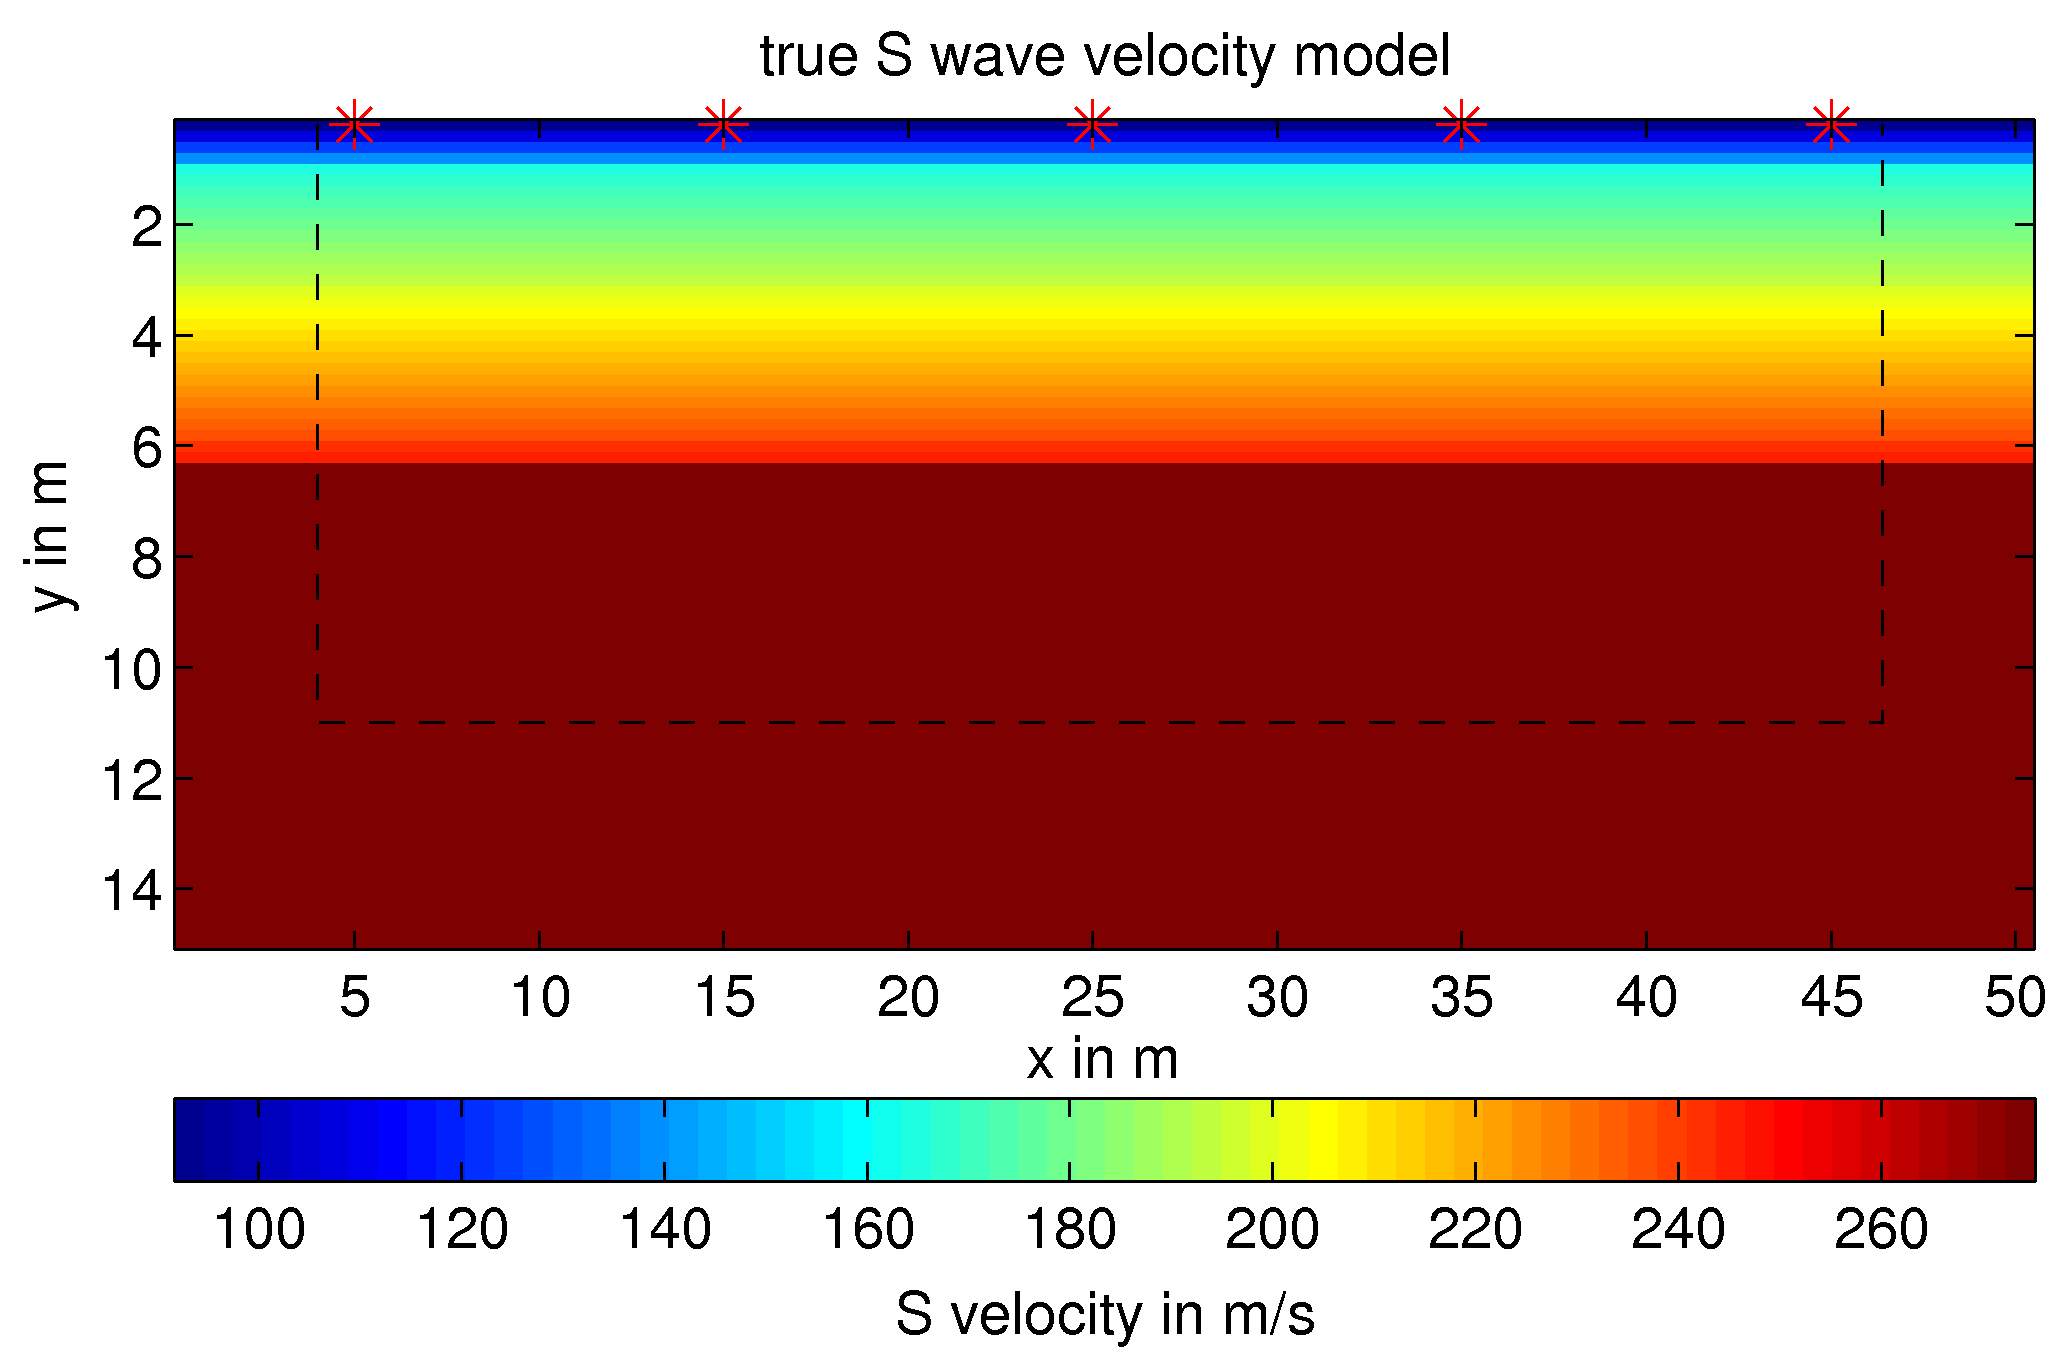
\includegraphics[width=10cm]{figures/Rheinstetten/true_vs_model}%
\label{true-vs-model-Rheinstetten}}\\%
\subfloat[][]{%
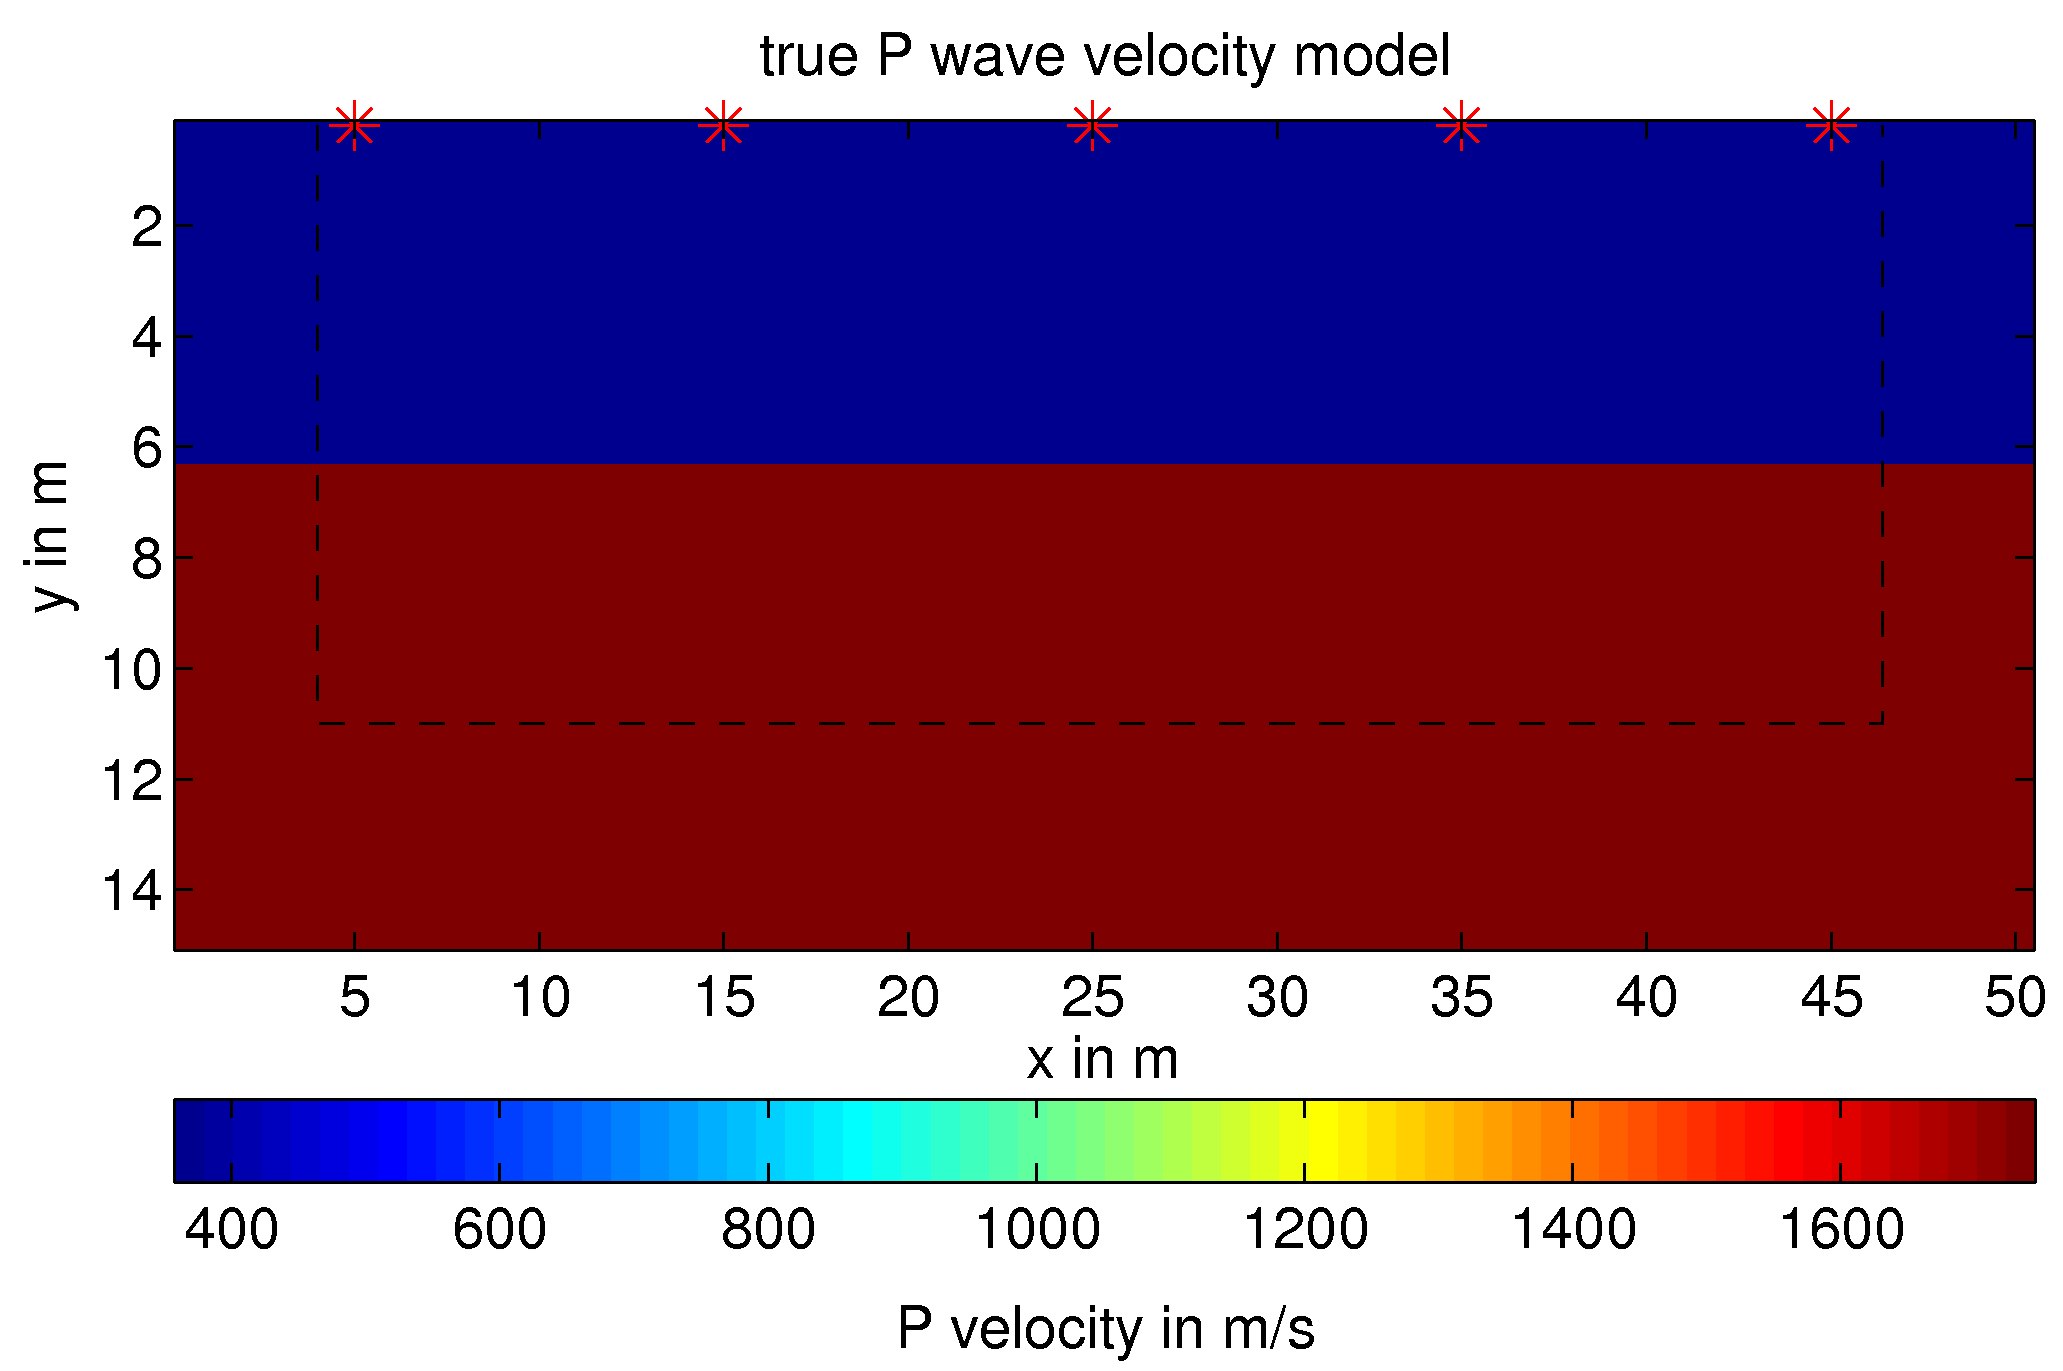
\includegraphics[width=10cm]{figures/Rheinstetten/true_vp_model}%
\label{true-vp-model-Rheinstetten}}\\%
\subfloat[][]{%
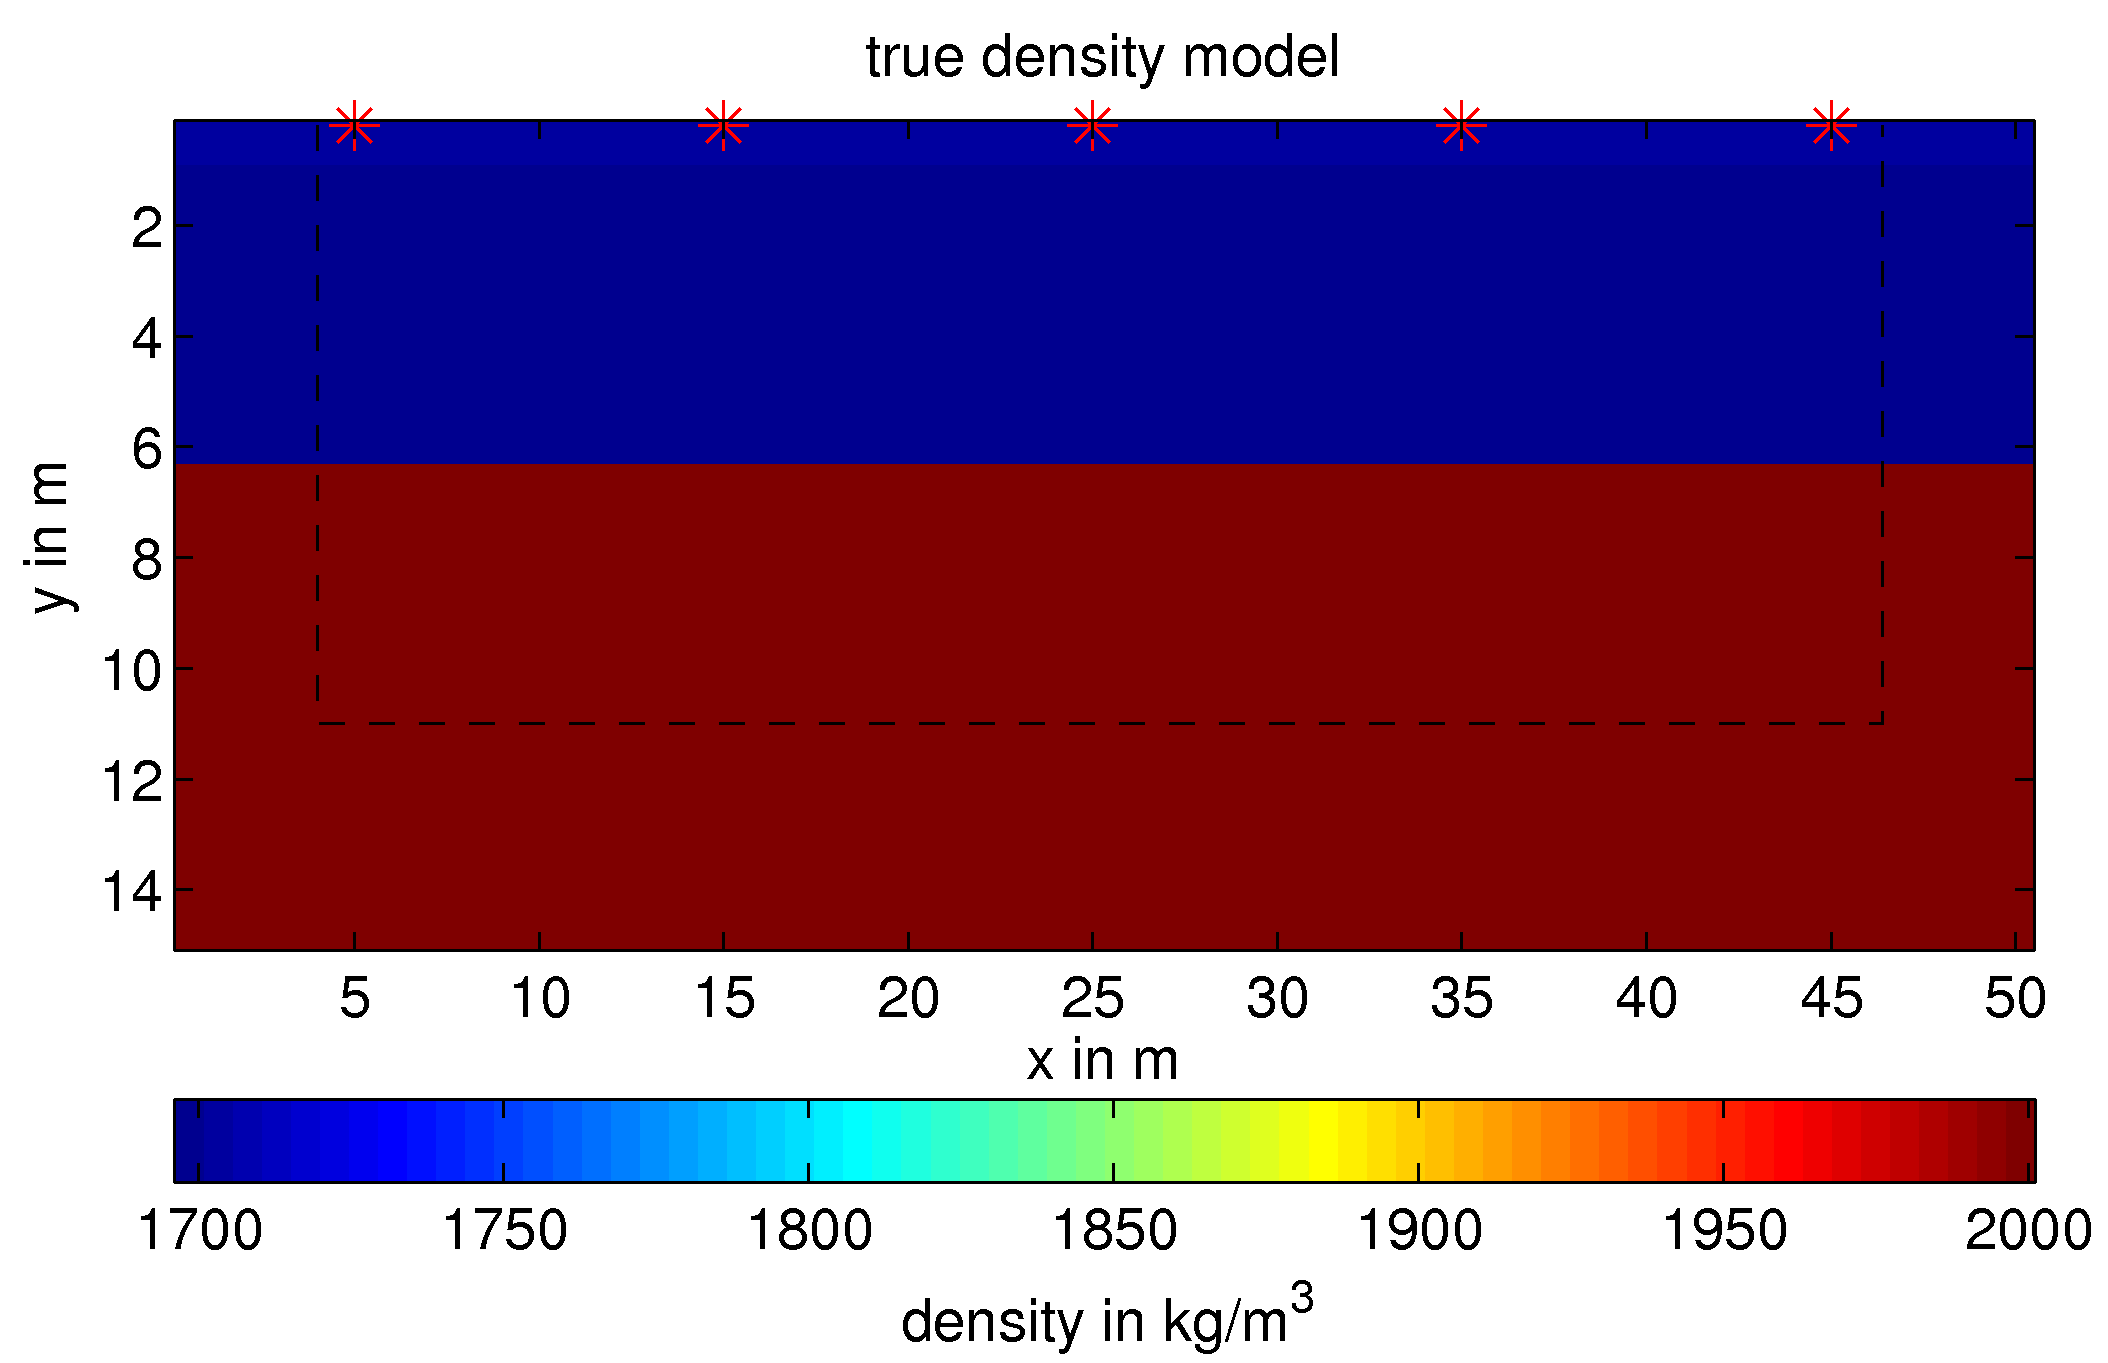
\includegraphics[width=10cm]{figures/Rheinstetten/true_rho_model}%
\label{true-rho-model-Rheinstetten}}
\caption{True models for \protect\subref{true-vs-model-Rheinstetten} the S wave velocity, \protect\subref{true-vp-model-Rheinstetten} the P wave velocity and \protect\subref{true-rho-model-Rheinstetten} the density used for the calculation of observed data. The red stars mark the five shots used in the inversion. The CPML frame is marked by the black dashed line.}
\label{Rheinstetten_true_model}
\end{figure}

\begin{figure}[ht]
\centering
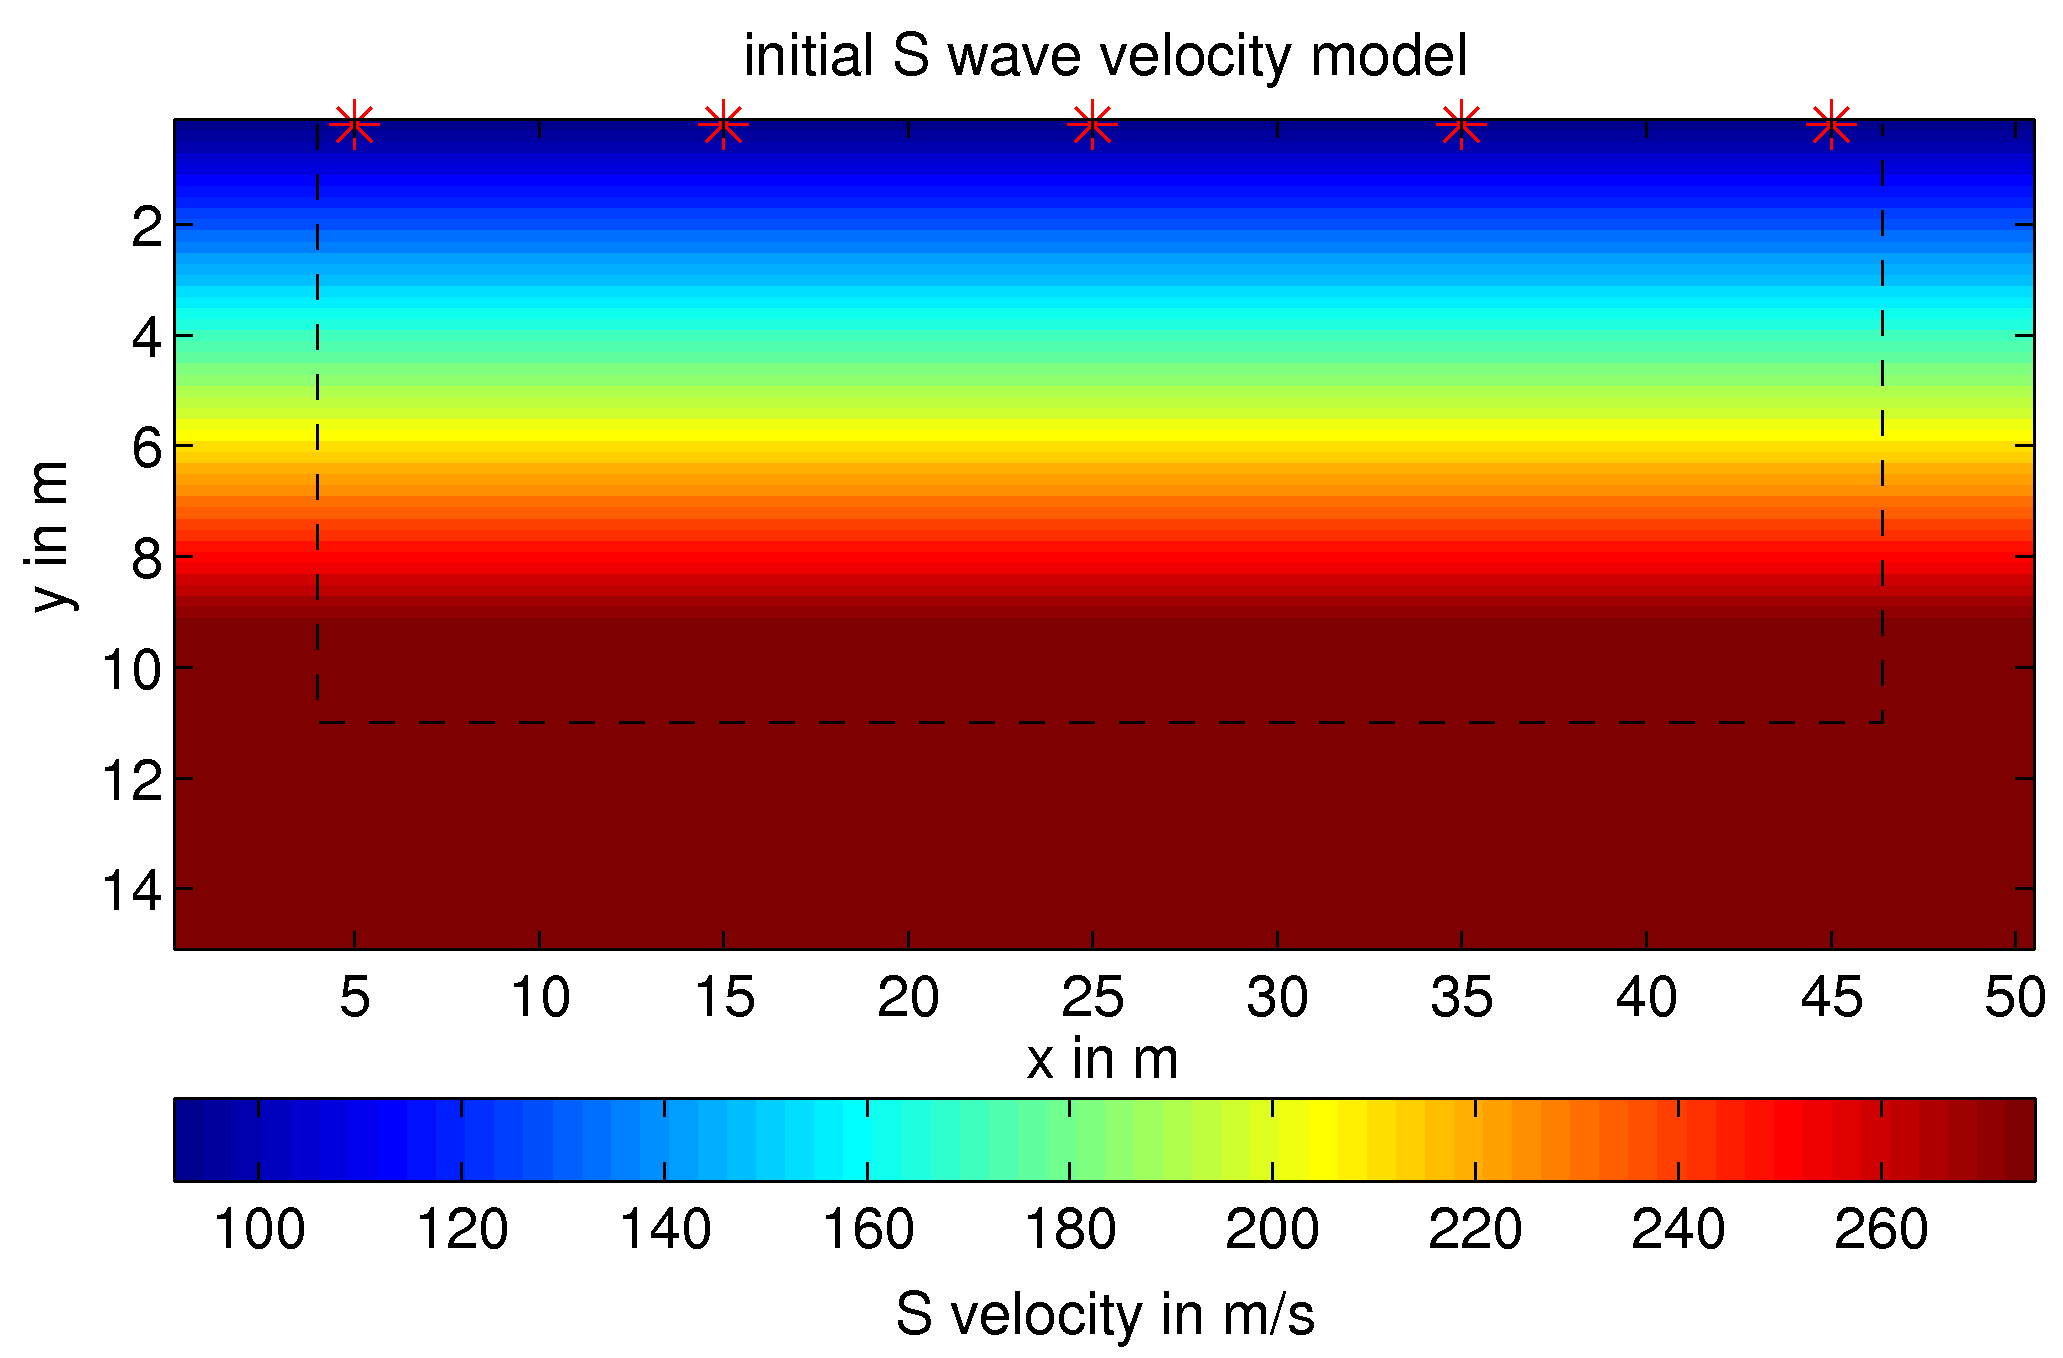
\includegraphics[width=10cm]{figures/Rheinstetten/start_vs_model}
\caption{Initial shear wave velocity model. The red stars mark the five shots used in the inversion. The CPML frame is marked by the black dashed line.}
\label{Rheinstetten_initial_vs_model}
\end{figure}

\begin{figure}[ht]
\centering
\subfloat[][]{%
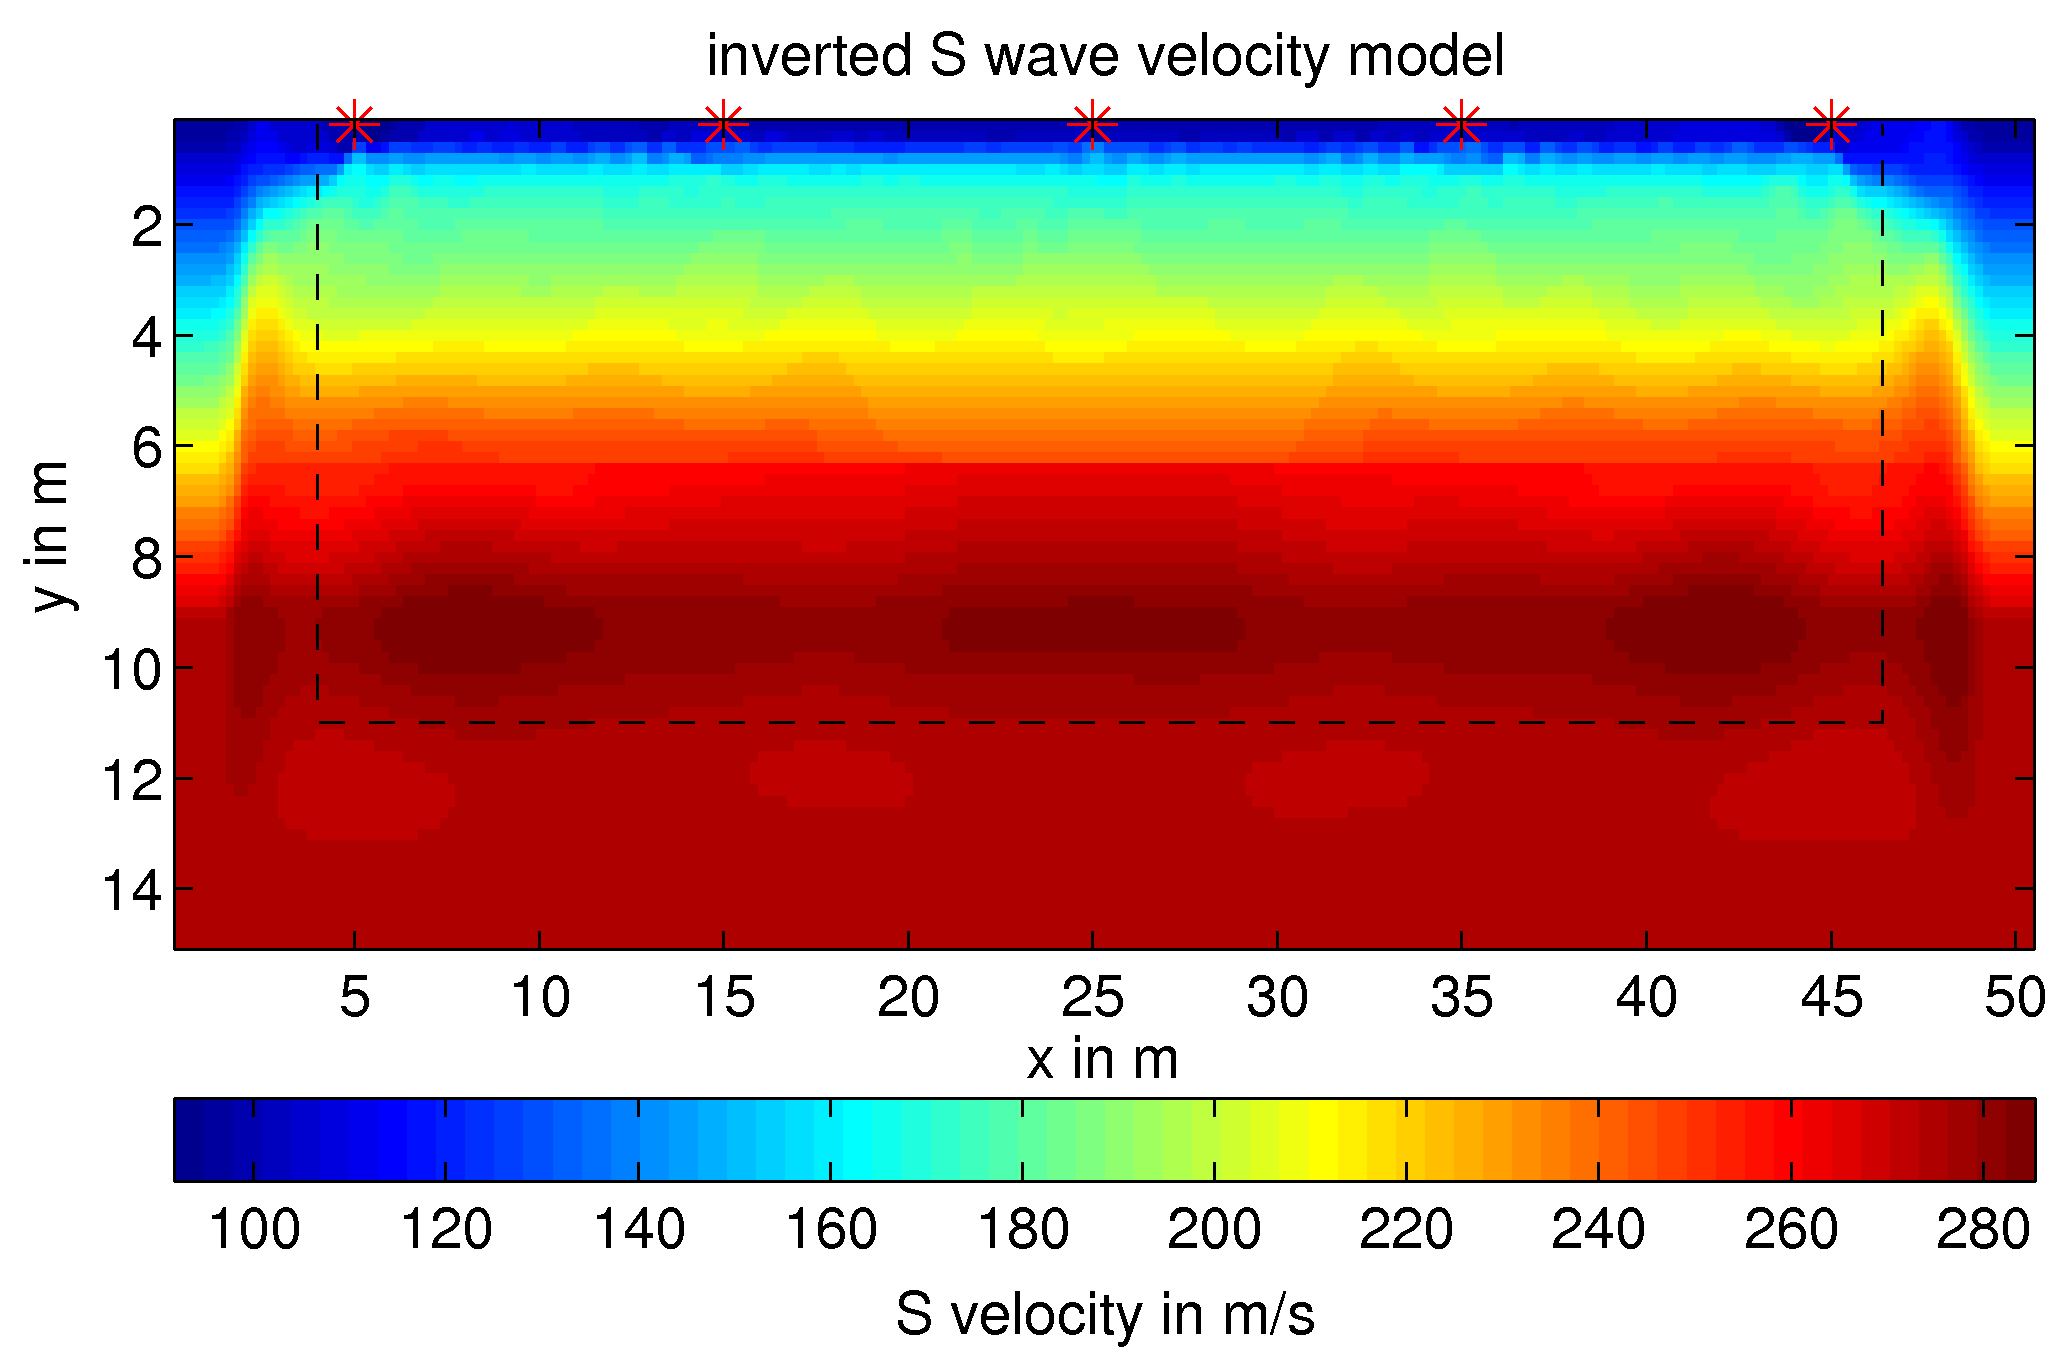
\includegraphics[width=10cm]{figures/Rheinstetten/inv_vs_model}%
\label{inv-vs-model-Rheinstetten}}%
\hspace{0.2 cm}
\subfloat[][]{%
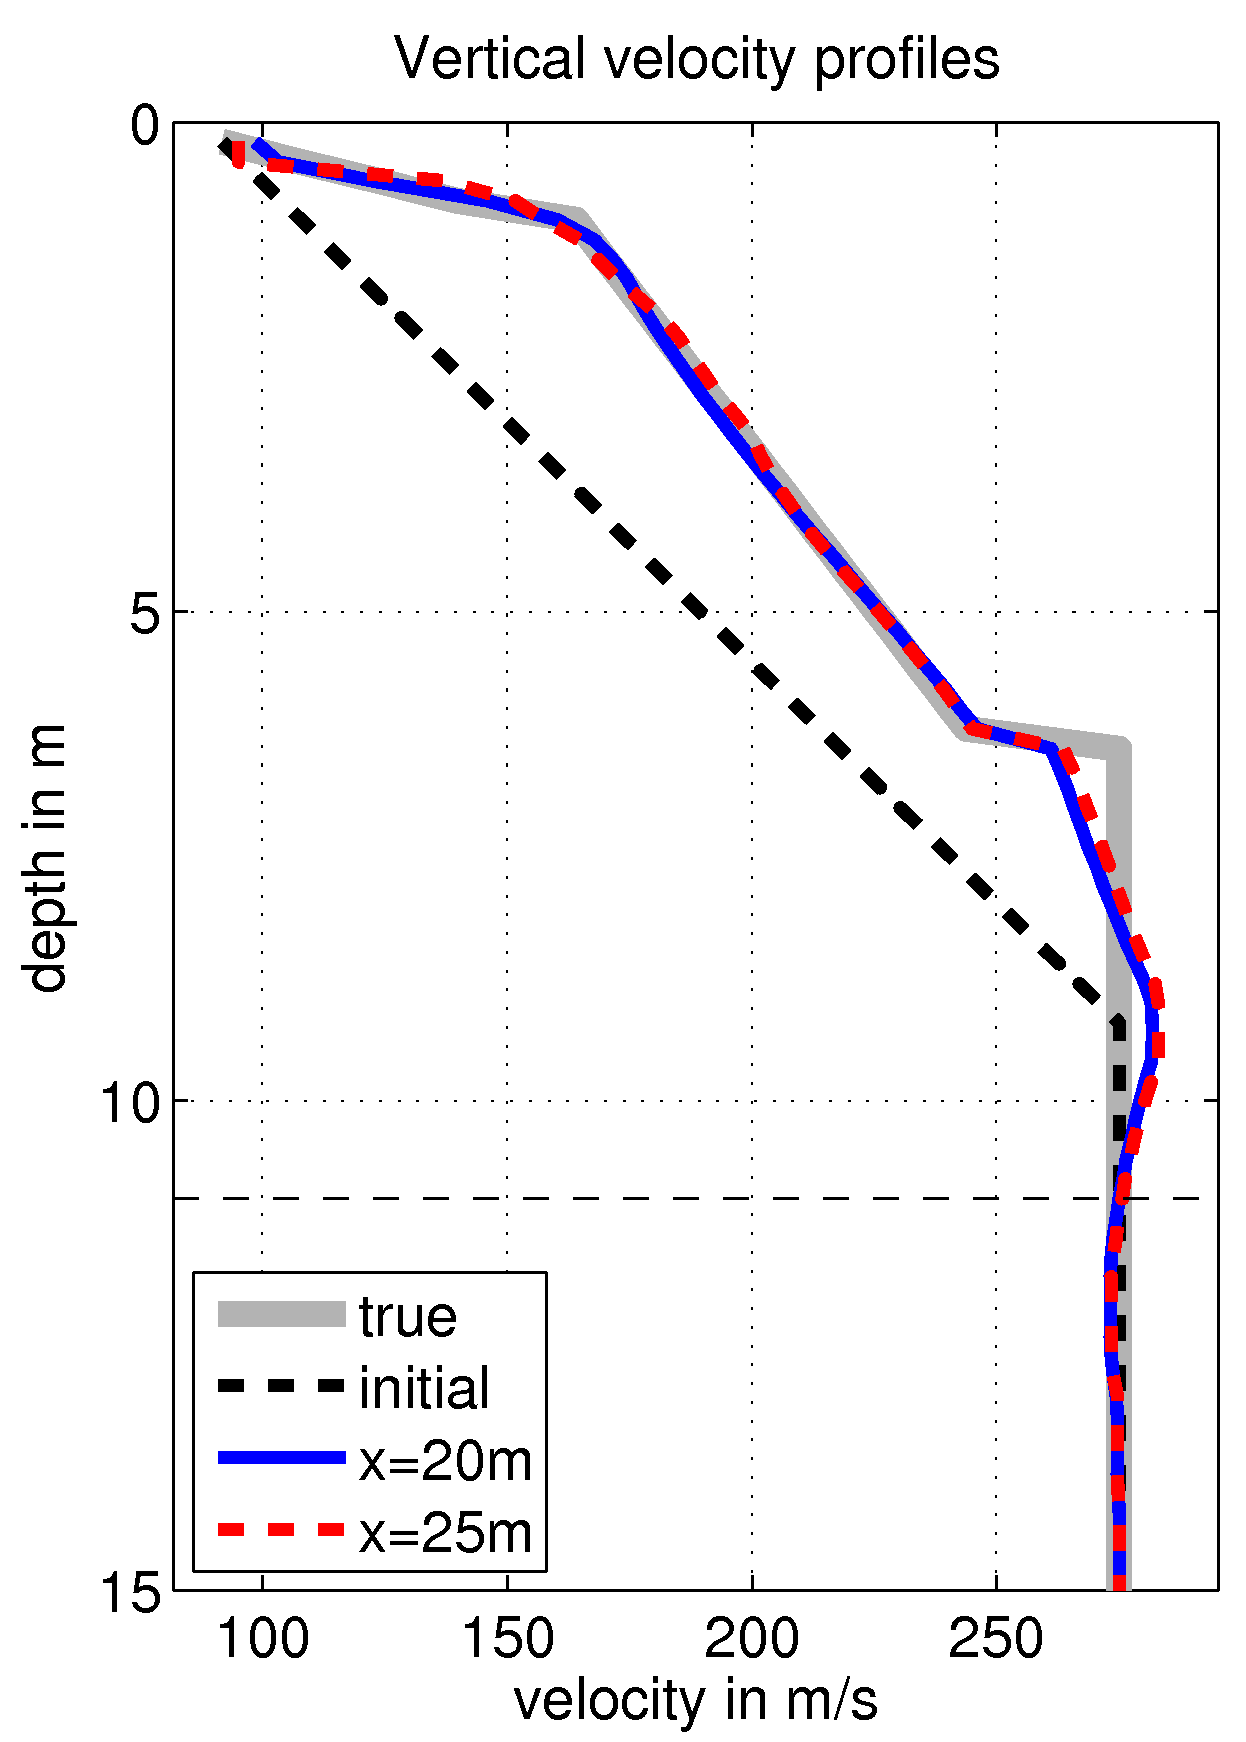
\includegraphics[width=5cm]{figures/Rheinstetten/vertical_vel_profiles}%
\label{vertical-vel-profiles-Rheinstetten}}
\caption{Inverted shear wave velocity model. \protect\subref{inv-vs-model-Rheinstetten} shows an imageplot of the inversion result. The red stars mark the source positions and the black dashed line marks the CPML frame. \protect\subref{vertical-vel-profiles-Rheinstetten} shows vertical velocity profiles of the shear wave velocity models. The true model is plotted with the thick grey line, the initial velocity model is represented by the dashed black line and two vertical profiles at $x$=20\,m and $x$=25\,m of the inverted model are plotted in red and blue. The CPML frame is again marked by the thin black line at 11\,m depth.}
\label{Rheinstetten_inversion_result}
\end{figure}

\clearpage


\bibliography{thesis}

%------------------------------------------------------------------------------------------------%

\appendix

\end{document}